\documentclass{amsart}

\usepackage[T1]{fontenc}
\usepackage{enumerate, amsmath, amsfonts, amssymb, amsthm, mathrsfs, wasysym, graphics, graphicx, xcolor, url, hyperref, hypcap, shuffle, xargs, multicol, overpic, pdflscape, multirow, hvfloat, minibox, accents, array, multido, xifthen, a4wide, ae, aecompl, blkarray, pifont, mathtools, etoolbox, dsfont, stmaryrd}
\usepackage{marginnote}
\hypersetup{colorlinks=true, citecolor=darkblue, linkcolor=darkblue}
\usepackage[all]{xy}
\usepackage[bottom]{footmisc}
\usepackage{tikz, tikz-cd, tikz-qtree}
\usetikzlibrary{trees, decorations, decorations.markings, shapes, arrows, matrix, calc, fit, intersections, patterns, angles, snakes}
\usepackage[external]{forest}
%\tikzexternalize
\graphicspath{{figures/}{figures/nodes/}}
\makeatletter\def\input@path{{figures/}}\makeatother
\usepackage{caption}
\captionsetup{width=\textwidth}
\renewcommand{\topfraction}{1} % possibility to have one page of pictures
\renewcommand{\bottomfraction}{1} % possibility to have one page of pictures
\usepackage[noabbrev,capitalise]{cleveref}
\usepackage[export]{adjustbox}
\usepackage{ulem}\normalem
\usepackage{xargs}

%%%%%%%%%%%%%%%%%%%%%%%%%%%%%%%%%%%%%%

% colors
\definecolor{darkblue}{rgb}{0,0,0.7} % darkblue color
\definecolor{green}{RGB}{57,181,74} % green color
\definecolor{violet}{RGB}{147,39,143} % violet color
\newcommand{\red}{\color{red}} % red command
\newcommand{\blue}{\color{blue}} % blue command
\newcommand{\orange}{\color{orange}} % orange command
\newcommand{\green}{\color{green}} % green command
\newcommand{\darkblue}{\color{darkblue}} % darkblue command

% marginal comments
\usepackage{todonotes}
\newcommand{\vincent}[1]{\todo[color=blue!30]{\rm #1 \\ \hfill --- V.}}
\newcommand{\vincenti}[1]{\todo[color=blue!30, inline]{\rm #1 \\ \hfill --- V.}}
\newcommand{\Guillaume}[1]{\todo[color=magenta!30]{\rm #1 \\ \hfill --- G.}}
\newcommand{\Kurt}[1]{\todo[color=orange!30]{\rm #1 \\ \hfill --- K.}}
\newcommand{\BDO}[1]{\todo[color=green!30]{\rm #1 \\ \hfill --- B.}}

% theorems
\newtheorem{theorem}{Theorem}[section]
\newtheorem*{theorem*}{Theorem}
\newtheorem{corollary}[theorem]{Corollary}
\newtheorem{proposition}[theorem]{Proposition}
\newtheorem{lemma}[theorem]{Lemma}
\newtheorem{conjecture}[theorem]{Conjecture}
\newtheorem{construction}[theorem]{Construction}

\theoremstyle{definition}
\newtheorem{definition}[theorem]{Definition}
\newtheorem{example}[theorem]{Example}
\newtheorem{remark}[theorem]{Remark}
\newtheorem{question}[theorem]{Question}
\newtheorem{problem}[theorem]{Problem}
\newtheorem{notation}[theorem]{Notation}
\newtheorem{assumption}[theorem]{Assumption}
\crefname{notation}{Notation}{Notations}
\crefname{problem}{Problem}{Problems}

% math special letters
\newcommand{\R}{\mathbb{R}} % reals
\newcommand{\N}{\mathbb{N}} % naturals
\newcommand{\Z}{\mathbb{Z}} % integers
\newcommand{\C}{\mathbb{C}} % complex
\newcommand{\I}{\mathbb{I}} % set of integers
\newcommand{\K}{\mathbb{K}} % field
\newcommand{\fA}{\mathfrak{A}} % alternating group
\newcommand{\fB}{\mathfrak{S}^\textsc{b}} % signed symmetric group
\newcommand{\cA}{\mathcal{A}} % algebra
\newcommand{\cC}{\mathcal{C}} % collection
\newcommand{\cS}{\mathcal{S}} % ground set
\newcommand{\uR}{\underline{R}} % underline set
\newcommand{\uS}{\underline{S}} % underline set
\newcommand{\uT}{\underline{T}} % underline set
\newcommand{\oS}{\overline{S}} % overline set
\newcommand{\ucS}{\underline{\cS}} % underline ground set
\renewcommand{\b}[1]{{\boldsymbol{#1}}} % bold letters
\newcommand{\bb}[1]{\mathbb{#1}} % bb letters
\newcommand{\f}[1]{\mathfrak{#1}} % frak letters
\newcommand{\h}{\widehat} % hat letters

% math commands
\newcommand{\set}[2]{\left\{ #1 \;\middle|\; #2 \right\}} % set notation
\newcommand{\bigset}[2]{\big\{ #1 \;\big|\; #2 \big\}} % big set notation
\newcommand{\Bigset}[2]{\Big\{ #1 \;\Big|\; #2 \Big\}} % Big set notation
\newcommand{\setangle}[2]{\left\langle #1 \;\middle|\; #2 \right\rangle} % set notation
\newcommand{\ssm}{\smallsetminus} % small set minus
\newcommand{\dotprod}[2]{\left\langle \, #1 \; \middle| \; #2 \, \right\rangle} % dot product
\newcommand{\symdif}{\,\triangle\,} % symmetric difference
\newcommand{\one}{\b{1}} % the all one vector
\newcommand{\eqdef}{\mbox{\,\raisebox{0.2ex}{\scriptsize\ensuremath{\mathrm:}}\ensuremath{=}\,}} % :=
\newcommand{\defeq}{\mbox{~\ensuremath{=}\raisebox{0.2ex}{\scriptsize\ensuremath{\mathrm:}} }} % =:
\newcommand{\simplex}{\b{\triangle}} % simplex
\renewcommand{\implies}{\Rightarrow} % imply sign
\newcommand{\transpose}[1]{{#1}^t} % transpose matrix
\renewcommand{\complement}[1]{\bar{#1}} % complement

% operators
\DeclareMathOperator{\conv}{conv} % convex hull
\DeclareMathOperator{\vect}{vect} % linear span
\DeclareMathOperator{\cone}{cone} % cone hull
\DeclareMathOperator{\inv}{inv} % inversions
\DeclareMathOperator{\Ima}{Im} %Image d'une fonction
\DeclareMathOperator{\std}{std}

% others
\newcommand{\ie}{\textit{i.e.}~} % id est
\newcommand{\eg}{\textit{e.g.}~} % exempli gratia
\newcommand{\Eg}{\textit{E.g.}~} % exempli gratia
\newcommand{\apriori}{\textit{a priori}} % a priori
\newcommand{\viceversa}{\textit{vice versa}} % vice versa
\newcommand{\versus}{\textit{vs.}~} % versus
\newcommand{\aka}{\textit{a.k.a.}~} % also known as
\newcommand{\perse}{\textit{per se}} % per se
\newcommand{\ordinal}{\textsuperscript{th}} % th for ordinals
\newcommand{\ordinalst}{\textsuperscript{st}} % st for ordinals
\newcommand{\defn}[1]{\textsl{\darkblue #1}} % emphasis of a definition
\newcommand{\para}[1]{\medskip\noindent\uline{#1.}} % paragraph
\renewcommand{\topfraction}{1} % possibility to have one page of pictures
\renewcommand{\bottomfraction}{1} % possibility to have one page of pictures
\newcommand{\imagetop}[1]{\vtop{\null\hbox{#1}}} % image aligned top
\newcommand{\OEIS}[1]{\cite[{\rm \href{http://oeis.org/#1}{\texttt{#1}}}]{OEIS}}

%Hyperplane arrangements
\renewcommand{\b}[1]{\boldsymbol{#1}} % bold
\newcommandx{\arrangement}[1][1 = A]{\mathcal{#1}} % arrangement
\newcommand{\HH}{\mathbb{H}} % hyperplane
\newcommandx{\braidArrangement}[1][1 = n]{\arrangement[B]_{#1}} % braid arrangement
\newcommandx{\multiBraidArrangement}[2][1 = n, 2 = \ell]{\arrangement[B]_{#1}^{#2}} % (l,n)-braid arrangement
\newcommandx{\rank}[1][1 = \arrangement]{\operatorname{rk}(#1)} % rank
\newcommandx{\facePoset}[1][1 = \arrangement]{\mathsf{Fa}(#1)} % face poset
\newcommandx{\fPol}[2][1 = \arrangement, 2 = x]{\b{f}_{#1}(#2)} % face polynomial
\newcommandx{\bPol}[2][1 = \arrangement, 2 = x]{\b{b}_{#1}(#2)} % bounded face polynomial
\newcommandx{\flatPoset}[1][1 = \arrangement]{\mathsf{Fl}(#1)} % intersection poset
\newcommandx{\charPol}[2][1 = \arrangement, 2 = y]{\b{\chi}_{#1}(#2)} % characteristic polynomial
\newcommandx{\mobPol}[3][1 = \arrangement, 2 = x, 3 = y]{\b{\mu}_{#1}(#2, #3)} % Mobius polynomial
\newcommandx{\partitionPoset}[1][1 = n]{\mathsf{Pa}_{#1}} % partition poset
\newcommandx{\forestPoset}[2][1 = n, 2 = \ell]{\mathsf{Fo}_{#1}^{#2}} % forest poset
\newcommandx{\rainbowForests}[2][1 = n, 2 = \ell]{\mathsf{RF}_{#1}^{#2}} % rainbow forests
\newcommandx{\rainbowTrees}[2][1 = n, 2 = \ell]{\mathsf{RT}_{#1}^{#2}} % rainbow trees
\newcommandx{\Perm}[1][1 = n]{\mathds{P}\mathsf{erm}(#1)} % permutahedron

%Operadic diagonals
\newcommand{\SU}{\mathrm{SU}}
\newcommand{\LA}{\mathrm{LA}}
\newcommand{\SUD}{\triangle^{\mathrm{SU}}}
\newcommand{\LAD}{\triangle^{\mathrm{LA}}}
\newcommand{\SCP}{\mathrm{SCP}}
\newcommand{\PolySub}{\mathsf{Poly}}
\newcommand{\EC}{\mathcal{E}} %essential complimentary partitions
\newcommand{\OP}{\triangle} %ordered partitions
\newcommand{\BT}{\mathcal{B}} %bipartite trees
\newcommand{\Ainf}{\ensuremath{\mathrm{A}_\infty}}
\newcommand{\op}{\mathrm{op}}
\newcommand{\tr}{\mathrm{tr}}
\newcommand{\id}{\mathrm{id}}

%Shift operators
%\vphantom{1} ensures sequential arrows aligned.
\newcommand{\rightshift}[1]{\overrightarrow{\vphantom{1}{#1}}}
\newcommand{\rightshiftk}[2]{\overrightarrow{\vphantom{1}{#1}}^{#2}}
\newcommand{\leftshift}[1]{\overleftarrow{\vphantom{1}{#1}}}
\newcommand{\leftshiftk}[2]{\overleftarrow{\vphantom{1}{#1}}^{#2}}
%Subdiv cube defs
\newcommand{\subdivpairsv}{e_v}
\newcommand{\maxsubdivpairsv}{\overline{e_v}}


% formating the table of contents
\setcounter{tocdepth}{2}
\makeatletter
\def\l@part{\@tocline{1}{8pt}{0pc}{}{}}
\def\l@section{\@tocline{1}{4pt}{0pc}{}{}}
\makeatother
\let\oldtocpart=\tocpart
\renewcommand{\tocpart}[2]{\sc\large\oldtocpart{#1}{#2}}
\let\oldtocsection=\tocsection
\renewcommand{\tocsection}[2]{\bf\oldtocsection{#1}{#2}}
\let\oldtocsubsubsection=\tocsubsubsection
\renewcommand{\tocsubsubsection}[2]{\quad\oldtocsubsubsection{#1}{#2}}

%%%%%%%%%%%%%%%%%%%%%%%%%%%%%%%%%%%%%%

\title{The combinatorics of the permutahedron diagonals}

\thanks{}

\author[B. Delcroix-Oger]{B\'er\'enice Delcroix-Oger}
\address{Institut Montpelli\'erain Alexander Grothendieck, Universit\'e de Montpellier, France}
\email{berenice.delcroix-oger@umontpellier.fr}
\urladdr{\url{https://oger.perso.math.cnrs.fr/}}

\author[M. Josuat-Verg\`es]{Matthieu Josuat-Verg\`es}
\address{}
\email{}

\author[G. Laplante-Anfossi]{Guillaume Laplante-Anfossi}
\address{School of Mathematics and Statistics, The University of Melbourne, Victoria, Australia}
\email{guillaume.laplanteanfossi@unimelb.edu.au}

\author[V. Pilaud]{Vincent Pilaud}
\address[Vincent Pilaud]{CNRS \& LIX, \'Ecole Polytechnique, Palaiseau}
\email{vincent.pilaud@lix.polytechnique.fr}
\urladdr{\url{http://www.lix.polytechnique.fr/~pilaud/}}

\author[K. Stoeckl]{Kurt Stoeckl}
\address{School of Mathematics and Statistics, The University of Melbourne, Victoria, Australia}
\email{kstoeckl@student.unimelb.edu.au}

%%%%%%%%%%%%%%%%%%%%%%%%%%%%%%%%%%%%%%

\begin{document}

\begin{abstract}
The purpose of this article is to provide a systematic combinatorial-geometric study of cellular diagonals on the permutahedra. 
First, we give general enumeration results for the faces of any geometric diagonal, using a theorem of Zavlasky on the M\"obius function of hyperplane arrangements.
The numbers obtained involve covering trees of bipartite graphs and Catalan families. 
Second, we prove that there are only two operadic families of diagonals on the permutahedra, and we give a bijection of their facets with planar bipartite trees and characterize their vertices as pattern-avoiding pairs of permutations.
A corollary of our study is that the Saneblidze--Umble diagonal can be recovered by a choice of vectors in the fundamental hyperplane arrangements of the permutahedra, resolving a conjecture of the third-named author.  
\end{abstract}

\vspace*{.1cm}
\maketitle

\tableofcontents

%%%%%%%%%%%%%%%%%%%%%%%%%%%%%%%%%%%%%%

\newpage
\section*{Introduction} 
\label{s:introduction}

In this article, discrete geometry \emph{informs} higher algebra.
First, we obtain some purely combinatorial results, whose study is motivated by higher algebra: the combinatorially inclined reader can read the first part of this introduction, and go directly to Section 1.
Second, we obtain some (higher) algebraic results via discrete geometry: the algebraically inclined reader can read the second part of this introduction, and go directly to Section 2.
\Guillaume{I am not sure this is the way to go anymore}

%%%%%%%%%%%%%%%

\subsection*{Motivation}

The purpose of this article is to study cellular diagonals on the permutahedra, which are cellular maps homotopic to the usual thin diagonal $\triangle : P \to P \times P, x \mapsto (x,x)$.
Such diagonals, and in particular coherent families that we call \emph{operadic} diagonals (see [DEF] \BDO{Reference ?}), are of interest in algebraic geometry and topology: via the theory of Fulton--Sturmfels \cite{fultonIntersectionTheoryToric1997a}, they give explicit formulas for the cup product on Losev--Manin toric varieties \cite{losevNewModuliSpaces2000}; they define universal tensor products of homotopy operads, and in particular universal tensor products of homotopy associative permutads (shuffle algebras) \cite{LA21}; they allow for the definition of a coproduct on permutahedral sets, which are used to models of two-fold loop spaces \cite{SaneblidzeUmble04}; and their study is moreover needed to pursue the work of Baues aiming at defining explicit combinatorial models for higher iterated loop spaces \cite{bauesGeometryLoopSpaces1980}. 
Moreover, using the canonical projections to the multiplihedra and the associahedra, they define universal tensor product of $\Ainf$-algebras and $\Ainf$-morphisms \cite{MazuirLA22}.
\Guillaume{lien avec les matroides?}

%%%%%%%%%%%%%%%

\subsection*{Combinatorics}

The purpose of the first part of this article is to study the combinatorics of the cellular diagonal of the permutohedra, explained in more details in the second part of the introduction.
 To make this part more accessible to non-algebraists, we formulate it in terms of hyperplane arrangements, as \emph{faces} of the cellular diagonal are in bijection with \emph{regions} of the associated hyperplane arrangements. 
 The hyperplane arrangement associated with  the cellular diagonal is two generically translated copies of the braid arrangement. 
 Motivated by the beautiful combinatorial formula obtained in our study, we generalize it to the study of $\ell$ generically translated copies of the braid arrangement, which would algebraically corresponds to some cellular $\ell$-gonal.
  We compute the $f$-vector and the $b$-vector of $\ell$-generically translated copies of the braid arrangement, using Zaslavsky's Theorem. 
  We refine the enumeration of the vertices of the hyperplane arrangement using a combinatorial interpretation in terms of $(\ell, n)$-trees and get the following multiplicative formula:
\begin{theorem}
For any~$k_1, \dots, k_\ell$ such that~$0 \le k_i \le n-1$ for~$i \in [\ell]$ and~${\sum_{i=1}^\ell k_i = n-1}$, the number of vertices~$v$ of the $(\ell,n)$-braid arrangement~$\multiBraidArrangement$ such that the smallest flat of the $i$\ordinal{} copy of~$\braidArrangement$ containing~$v$ has dimension~$n-k_i-1$ is given by
\[
n^{\ell-1} \binom{n-1}{k_1, \dots, k_\ell} \prod_{i=1}^\ell (n-k_i)^{k_i-1}.
\]
\end{theorem}

%%%%%%%%%%%%%%%

\subsection*{Higher Algebra}

The first cellular diagonal for the permutahedra was defined at the level of chains by S. Saneblidze and R. Umble in \cite{SaneblidzeUmble04}, we will call it the \emph{SU diagonal}. 
Cellular diagonals for the associahedra and the multiplihedra were also defined there, via projection. 
The first topological map for the permutahedra was given in \cite{LA21} -we will call it the \emph{LA diagonal}, where a general theory of cellular diagonals of polytopes was developed. 
The LA diagonal, however, is distinct from the SU diagonal at the cellular level \cite[Remark 3.19]{LA21}. 

computer program for the SU diagonal \cite{vejdemo-johanssonEnumeratingSaneblidzeUmbleDiagonal2007}; we give a much more effective computer program (however, without the signs)

corollary: le dernier article de SU!
corollary: IJ-description of SU diagonal
corollary: left and right shifts for LA, decomposition of the cube associated to LA diagonal

\Kurt{Mention the LAD and SUD shifts generate the (same) facets of the hexagon in two different ways.}

Perspectives: 
-for general diagonal, obtain closed formulas for all the faces
-for specific diagonals, extend the bijection with bipartite trees

%%%%%%%%%%%%%%%

\subsection*{Conventions}

%We use the notations of \cite{LodayVallette12} for operads.

\Guillaume{Please make a new line for each sentence as to facilitate comparison between versions in GitHub}

\Guillaume{Would it be possible to avoid bold letters, use "slash emph\{\}", and also reduce to the maximum possible the use of indices; as soon as the context is clear, drop any extra index}

\begin{table}[h]
	\centerline{
		\begin{tabular}{c|c|rrrrrrr|l}
			\textbf{Pairs $(F,G) \in \Ima\triangle_{(P,\vec v)}$} & \textbf{Polytopes} & \textbf{0} & \textbf{1} & \textbf{2} & \textbf{3} & \textbf{4} & \textbf{5} & \textbf{6} & \textbf{\cite{OEIS}} \\
			\hline
			& \text{Associahedra} & 1 & 2 & 6 & 22 & 91 & 408 & 1938 & \OEIS{A000139}  \\
			$ \dim F + \dim G = \dim P$  & \text{Multiplihedra} & 1 & 2 & 8 & 42 & 254 & 1678 & 11790 &  to appear \\
			& \text{Permutahedra} & 1 & 2 & 8 & 50 & 432 & 4802 & 65536 &  \OEIS{A007334} \\
			\hline
			& \text{Associahedra} & 1 & 3 & 13 & 68 & 399 & 2530 & 16965 &  \OEIS{A000260} \\
			$\dim F=\dim G =0$ & \text{Multiplihedra} & 1 & 3 & 17 & 122 & 992 & 8721 & 80920 & to appear \\
			& \text{Permutahedra} & 1 & 3 & 17 & 149 & 1809 & 28399 & 550297 &  \OEIS{A213507} 
		\end{tabular}
	}
	\caption{Number of pairs of faces in the cellular image of the diagonal of the associahedra, multiplihedra and permutahedra of dimension $0\leq \dim P \leq 6$, induced by any good orientation vector.}
	\label{table:numerology}
\end{table}

%%%%%%%%%%%%%%%%%%%%%%%%%%%%%%%%%%%%%%

\newpage
\section{Combinatorics of multiple braid arrangements}
\label{sec:combinatorics}

In this section, we study the combinatorics of hyperplane arrangements obtained as unions of generically translated copies of the braid arrangement.
%Specializing to two copies, we derive enumerative results on the diagonals of the permutahedra.

%%%%%%%%%%%%%%%

\subsection{Recollection on hyperplane arrangements}
\label{subsec:arrangements}

We first briefly recall classical results on the combinatorics of affine hyperplane arrangements, in particular the enumerative connection between their intersection posets and their face lattices due to T.~Zaslavsky~\cite{Zaslavsky}.

\begin{definition}
A (finite affine real) \defn{hyperplane arrangement} is a finite set~$\arrangement$ of affine hyperplanes in~$\R^d$.
\end{definition}

\begin{definition}
A \defn{region} of~$\arrangement$ is a connected component of~$\R^d \ssm \bigcup_{H \in \arrangement} H$.
A \defn{face} of~$\arrangement$ is the intersection of the closure of a region of~$\arrangement$ with an hyperplane of~$\arrangement$.
The \defn{face poset} of~$\arrangement$ is the poset~$\facePoset$ of faces of~$\arrangement$ ordered by inclusion.
The \defn{$f$-polynomial}~$\fPol$ and \defn{$b$-polynomial}~$\bPol$ of~$\arrangement$ are the polynomial
\[
\fPol \eqdef \sum_{k = 0}^d f_k(\arrangement) \, x^k
\qquad\text{and}\qquad
\bPol \eqdef \sum_{k = 0}^d b_k(\arrangement) \, x^k \, ,
\]
where~$f_k(\arrangement)$ denotes the number of $k$-dimensional faces of~$\arrangement$, while~$b_k(\arrangement)$ denotes the number of bounded $k$-dimensional faces of~$\arrangement$.
\end{definition}

\begin{definition}
A \defn{flat} of~$\arrangement$ is a non-empty affine subspace of~$\R^d$ that can be obtained as the intersection of some hyperplanes of~$\arrangement$.
The \defn{flat poset} of~$\arrangement$ is poset~$\flatPoset$ of flats of~$\arrangement$ ordered by reverse inclusion.
\end{definition}

\begin{definition}
\label{def:MobiusPolynomial}
%The \defn{characteristic polynomial}~$\chi_{\arrangement}(y)$ and the \defn{M\"obius polynomial}~$\mu_{\arrangement}(x,y)$ are the polynomials respectively defined by
%\[
%\charPol \eqdef \sum_{G \in \flatPoset} \mu_{\flatPoset}(\R^d, G) \, y^{\dim(G)}
%\quad\text{and}\quad
%\mobPol \eqdef \sum_{F \le G \in \flatPoset} \mu_{\flatPoset}(F,G) \, x^{\dim(F)} \, y^{\dim(G)}
%\]
The \defn{M\"obius polynomial}~$\mu_{\arrangement}(x,y)$ is the polynomial defined by
\[
\mobPol \eqdef \sum_{F \le G} \mu_{\flatPoset}(F,G) \, x^{\dim(F)} \, y^{\dim(G)},
\]
where~$F \le G$ ranges over all intervals of the flat poset~$\flatPoset$, and~$\mu_{\flatPoset}(F,G)$ denotes the \defn{M\"obius function} on the flat poset~$\flatPoset$ defined as usual by
\[
\mu_{\flatPoset}(F, F) = 1
\qquad\text{and}\qquad
\sum_{F \le G \le H} \mu_{\flatPoset}(F,G) = 0
\]
for all~$F, G, H \in \flatPoset$.
\end{definition}

\begin{remark}
Our definition of the M\"obius polynomial slightly differs from that of \cite{Zaslavsky} as we use the dimension of~$F$ instead of its codimension, in order for the next statement to be slightly simpler.
\end{remark}

\begin{theorem}[{\cite[Thm.~A]{Zaslavsky}}]
\label{thm:Zaslavsky}
The $f$-polynomial, the $b$-polynomial, and the M\"obius polynomial of an arrangement~$\arrangement$ are related by
\[
\fPol = \mobPol[\arrangement][-x][-1]
\qquad\text{and}\qquad
\bPol = \mobPol[\arrangement][-x][1].
\]
\end{theorem}

\begin{example}
For the arrangement~$\arrangement$ of $5$ hyperplanes of \cref{fig:arrangement}, we have
\[
\mobPol = x^2y^2 - 5x^2y + 6x^2 + 5xy - 10x + 4 \, ,
\]
so that
\begin{align*}
\fPol & = \mobPol[\arrangement][-x][-1] = 12 \, x^2 + 15 \, x + 4 \\
\text{and}\qquad
\bPol & = \mobPol[\arrangement][-x][1] = 2 \, x^2 + 5 \, x + 4.
\end{align*}
%
\begin{figure}
%	\begin{overpic}[scale=.9]{intersectionPoset}
%		\put(72.5, -2){$1$}
%		\put(51, 10){$-1$}
%		\put(61, 10){$-1$}
%		\put(71, 10){$-1$}
%		\put(82, 10){$-1$}
%		\put(94, 10){$-1$}
%		\put(51.5, 32){$2$}
%		\put(66, 32){$1$}
%		\put(80, 32){$1$}
%		\put(93.5, 32){$2$}
%	\end{overpic}
%	\caption{A hyperplane arrangement (left) and its intersection poset with its M\"obius function (right).}
	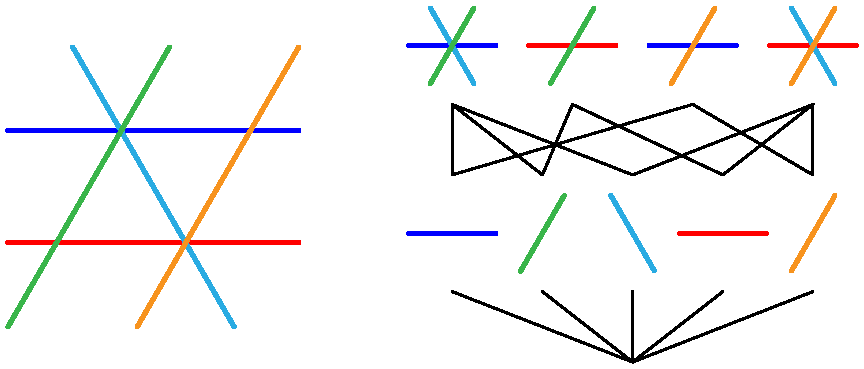
\includegraphics[scale=.9]{intersectionPoset}
	\caption{A hyperplane arrangement (left) and its intersection poset (right).}
	\label{fig:arrangement}
\end{figure}
\end{example}

\begin{remark}
\label{rem:characteristicPolynomial}
The coefficient of~$x^d$ in the M\"obius polynomial~$\mobPol$ gives the more classical \defn{characteristic polynomial}
\[
\charPol \eqdef [x^d] \, \mobPol = \sum_F \mu_{\flatPoset}(\R^d,F) \, y^{\dim(F)}.
\]
By \cref{thm:Zaslavsky}, we thus have
\[
f_d(\arrangement) = (-1)^d \, \charPol[\arrangement][-1] 
\qquad\text{and}\qquad
b_d(\arrangement) = (-1)^d \, \charPol[\arrangement][1].
\]
\end{remark}

%%%%%%%%%%%%%%%

\subsection{The braid arrangement}
\label{subsec:braidArrangement}

We now briefly recall the classical combinatorics of the braid arrangement.
\vincent{add refs?}

%\begin{figure}
%	\centerline{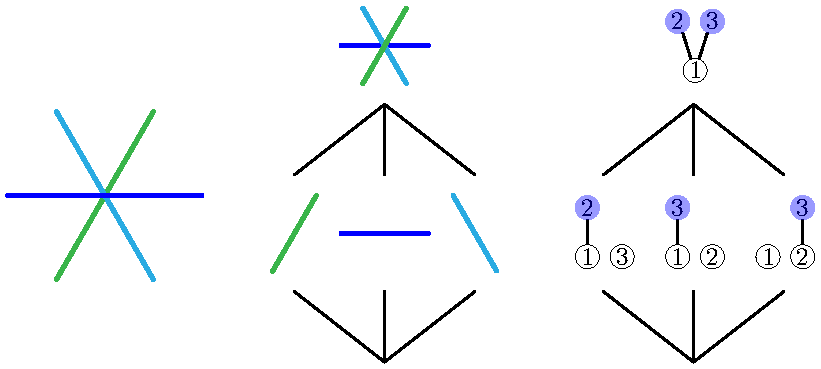
\includegraphics[scale=.9]{figures/intersectionPosetBraidArrangement3Full}}
%	\caption{The braid arrangement $\braidArrangement[3]$ (left), its flat poset~$\flatPoset[{\braidArrangement[3]}]$ (middle), and the partition poset~$\partitionPoset[3]$ (right).}
%	\label{fig:braidArrangement3}
%\end{figure}

\begin{figure}
	\centerline{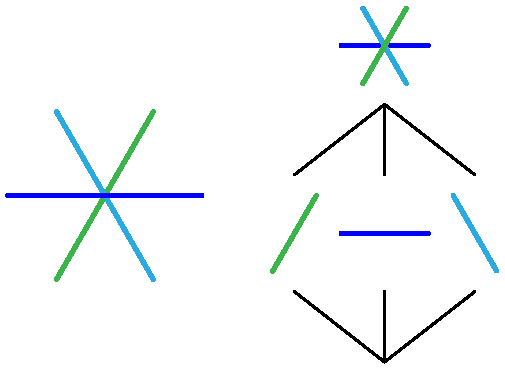
\includegraphics[scale=.9]{figures/intersectionPosetBraidArrangement3}}
	\caption{The flat poset of the braid arrangement $\braidArrangement[3]$, where flats are represented as intersections of hyperplanes (left) or as partitions of~$[3]$ (right).}
	\label{fig:intersectionPosetBraidArrangement3}
\end{figure}

\begin{figure}
	\centerline{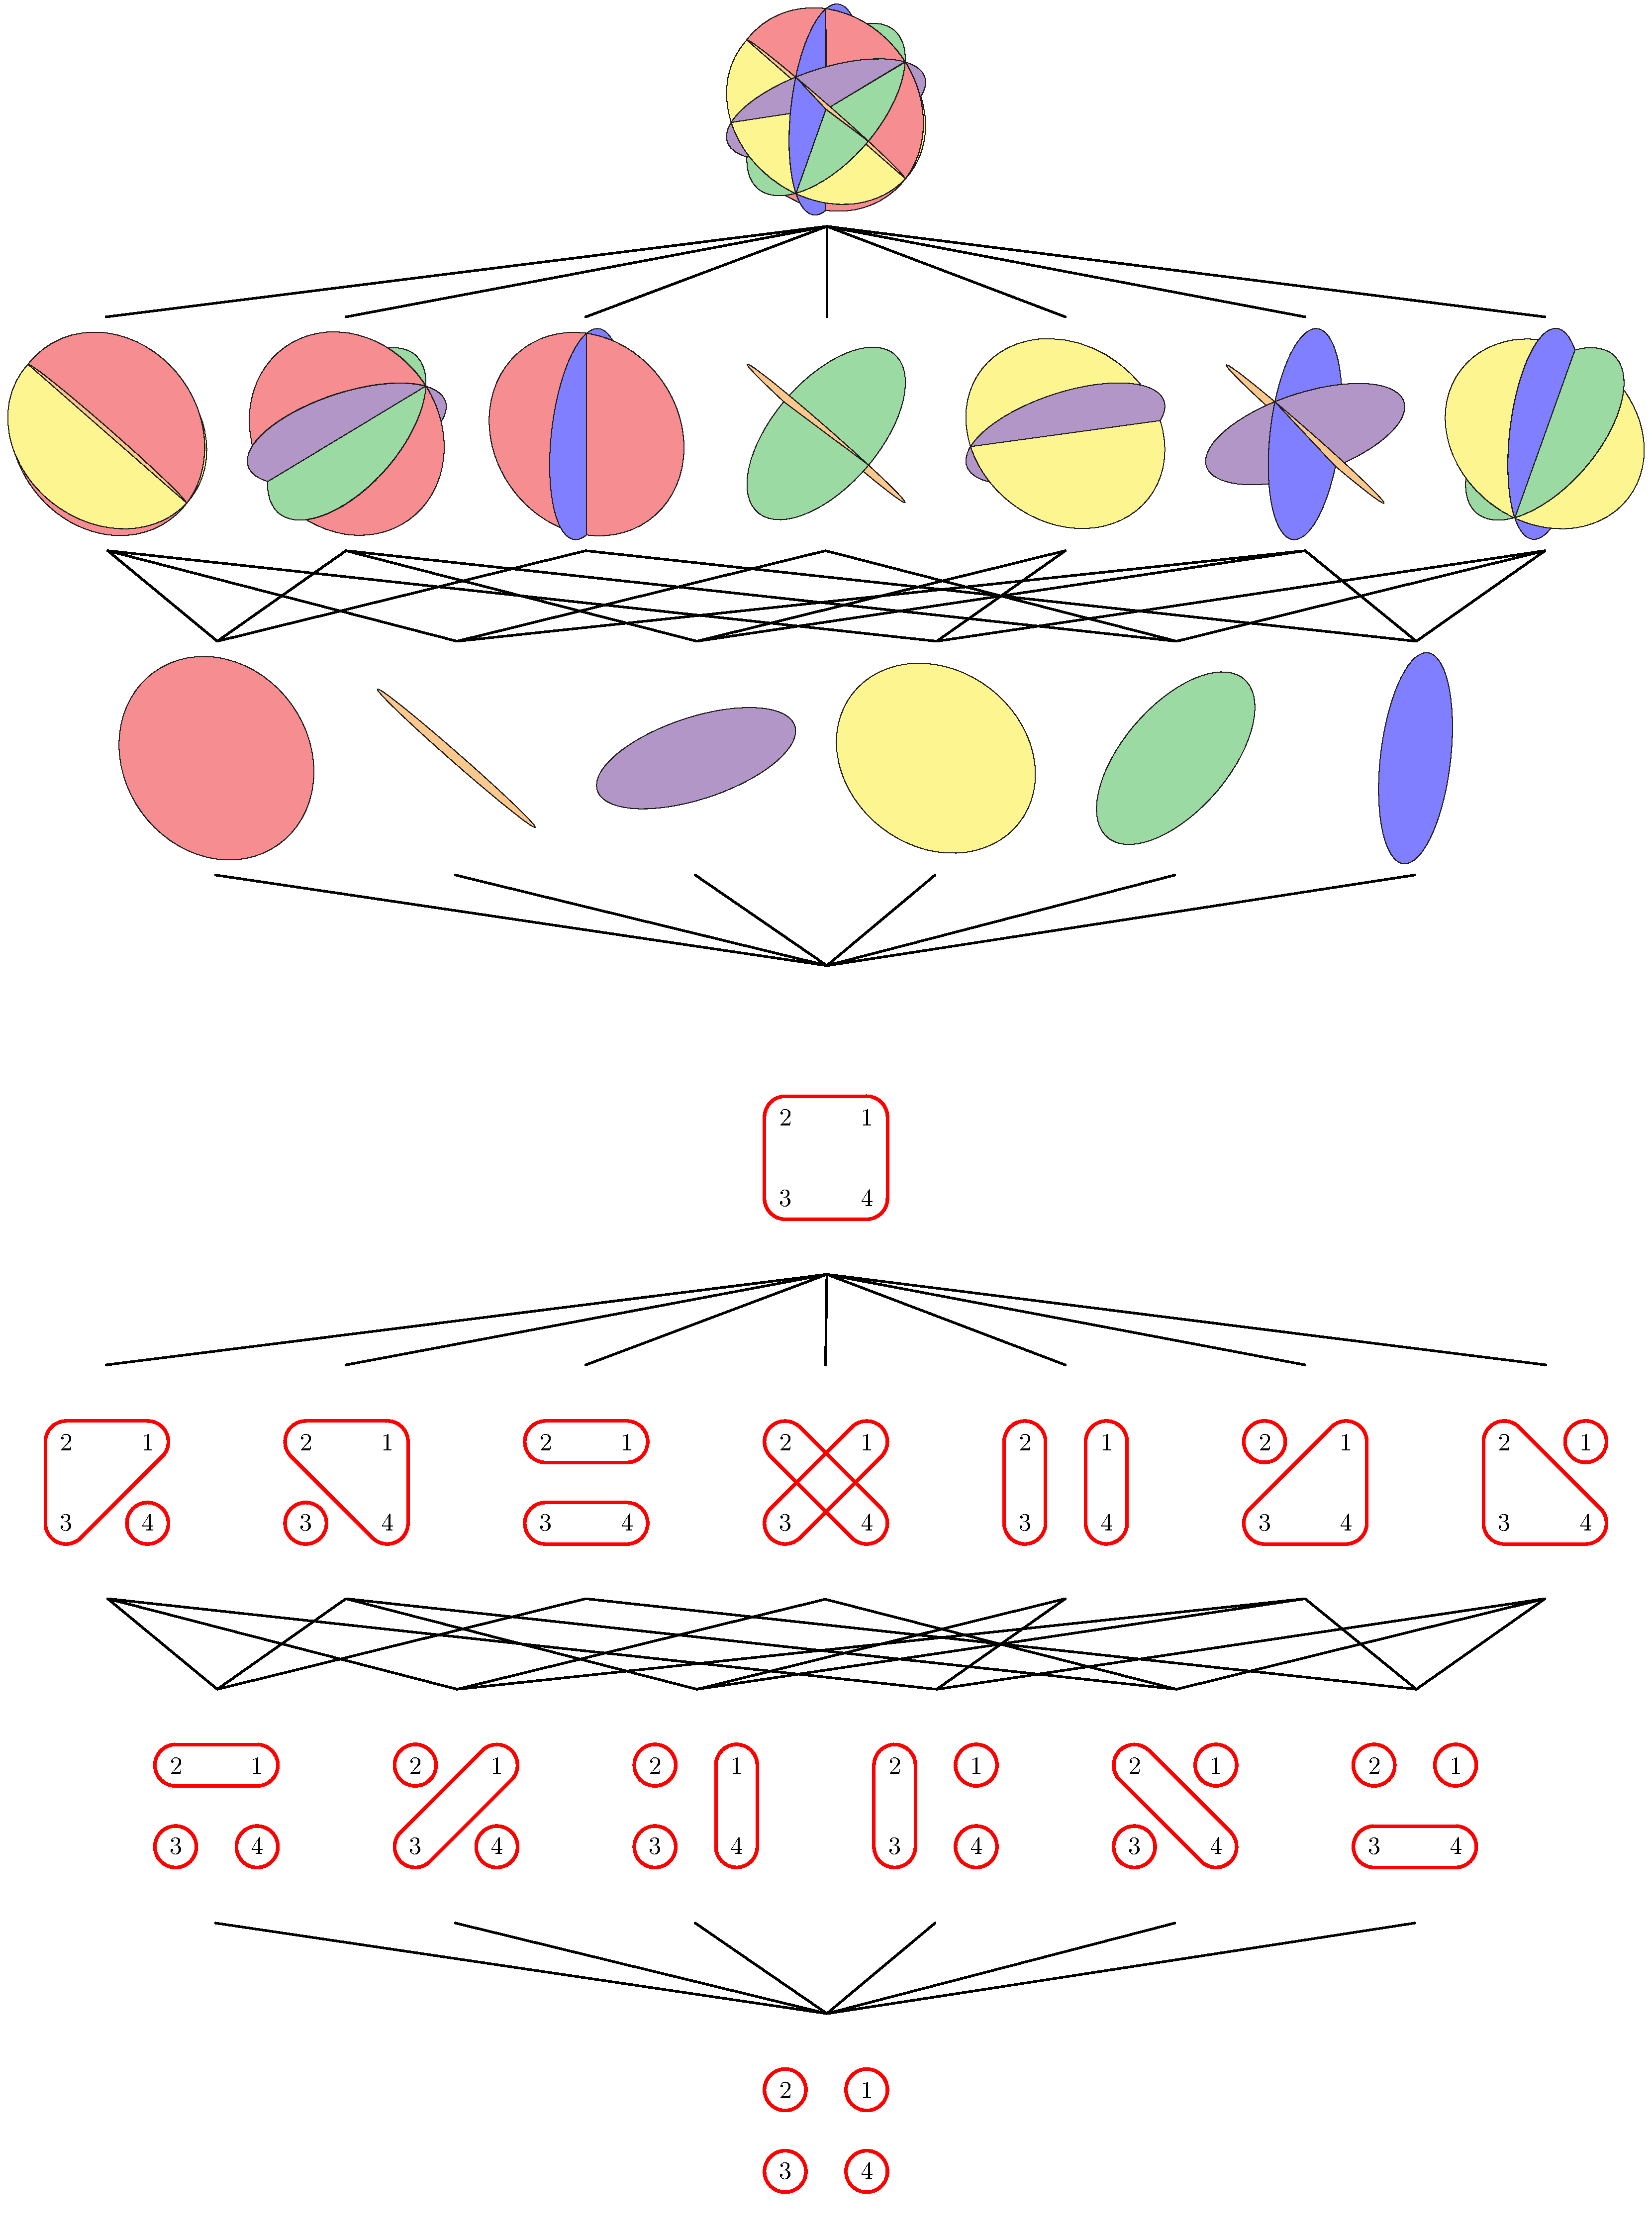
\includegraphics[scale=.26]{figures/intersectionPosetBraidArrangement4}}
	\caption{The flat poset of the braid arrangement $\braidArrangement[4]$, where flats are represented as intersections of hyperplanes (top) or as partitions of~$[4]$ (bottom).}
	\label{fig:intersectionPosetBraidArrangement4}
\end{figure}

\vincenti{Conceptually, it would be nicer in \cref{fig:intersectionPosetBraidArrangement4} to place the numbers $1,2,3,4$ on the vertices of the regular tetrahedron corresponding to the braid arrangement (as is done in \cref{fig:intersectionPosetBraidArrangement3}). However, this is visually not as nice, so I have decided to put them on a squarre.}

\begin{definition}
Fix~$n \ge 1$ and denote by~$\HH$ the hyperplane of~$\R^n$ defined by~$\sum_{r = 1}^n x_r = 0$.
The \defn{braid arrangement}~$\braidArrangement$ is the arrangement of the hyperplanes~$\set{\b{x} \in \HH}{x_r = x_s}$ for all~$1 \le r < s \le n$.
\end{definition}

\begin{remark}
\label{rem:essential}
Note that we have decided to work in the space~$\HH$ rather than in the space~$\R^n$.
The advantage is that the braid arrangement~$\braidArrangement$ is essential, so that we can speak of its vertices.
Working in~$\R^n$ would change vertices to rays, and would multiply all M\"obius polynomials by a factor~$xy$.
\end{remark}

The combinatorics of the braid arrangement~$\braidArrangement$ is well-known.
It has a $k$-dimensional~flat
\[
\Psi(\pi) \eqdef \set{\b{x} \in \R^n}{x_r = x_s \text{ for all } r, s \in p \in \pi}
\]
for each set partition~$\pi$ of~$[n]$ into $k+1$ parts.
The flat poset~$\flatPoset[\braidArrangement]$ is thus the refinement poset~$\partitionPoset$ \BDO{$\Pi_n$ ?} on set partitions of~$[n]$ (where a partition~$\pi$ is smaller than a partition~$\omega$ if each part of~$\pi$ is contained in a part of~$\omega$).
For instance, \cref{fig:intersectionPosetBraidArrangement3,fig:intersectionPosetBraidArrangement4} illustrate the flat posets of the braid arrangements~$\braidArrangement[3]$ and~$\braidArrangement[4]$.
The M\"obius function of~$\partitionPoset$ is given by
\[
\mu_{\partitionPoset}(\pi, \omega) = \prod_{p \in \omega} (-1)^{\#\pi[p]-1}(\#\pi[p]-1)! \, ,
\]
where~$\pi[p]$ denotes the restriction of the partition~$\pi$ to the part~$p$ of the partition~$\omega$, and $\#\pi[p]$ denotes its number of parts.
See for instance \cite{Birkhoff, Rota}.
The M\"obius polynomial of the braid arrangement~$\braidArrangement$ is given by
\[
\mobPol[\braidArrangement] = \sum_{k \in [n]} x^{k-1} S(n,k) \prod_{i \in [k-1]} (y-i) \, ,
\]
where~$S(n,k)$ denotes the Stirling number of second kind \OEIS{A008277}, \ie the number of set partitions of~$[n]$ into~$k$ parts.
For instance
\begin{align*}
\mobPol[{\braidArrangement[1]}] & = 1 \\
\mobPol[{\braidArrangement[2]}] & = x y - x + 1 = x (y - 1) + 1 \\
\mobPol[{\braidArrangement[3]}] & = x^2 y^2 - 3 x^2 y + 2 x^2 + 3 x y - 3 x + 1 = x^2 (y - 1) (y - 2) + 3 x (y - 1) + 1\\
\mobPol[{\braidArrangement[4]}] & = x^3 y^3 - 6 x^3 y^2 + 11 x^3 y - 6 x^3 + 6 x^2 y^2 - 18 x^2 y + 12 x^2 + 7 x y - 7 x + 1 \\
& = x^3 (y - 1) (y - 2) (y - 3) + 6 x^2 (y - 1) (y - 2) + 7 x (y - 1) + 1.
\end{align*}
In particular, the characteristic polynomial of the braid arrangement~$\braidArrangement$ is given by
\[
\charPol[\braidArrangement] = (y-1) (y-2) \dots (y-n-1).
\]
Working in~$\R^n$ rather than in~$\HH$ would lead to an additional~$y$ factor in this formula, which might be more familiar to the reader
See \cref{rem:essential}.

%%%%%%%%%%%%%%%

\subsection{The $(\ell,n)$-braid arrrangement}
\label{subsec:multiBraidArrangement}

We now focus on the following specific hyperplane arrangements, illustrated in \cref{fig:multiBraidArrangements}.

\begin{figure}[t]
	\centerline{
	\begin{tabular}{c@{\hspace{.7cm}}c@{\hspace{.7cm}}c@{\hspace{.7cm}}c}
		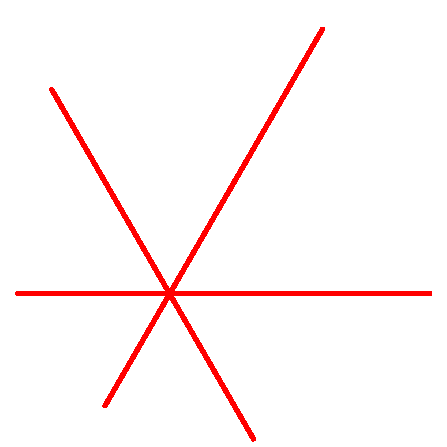
\includegraphics[scale=.4]{multiBraidArrangement1}
		&
		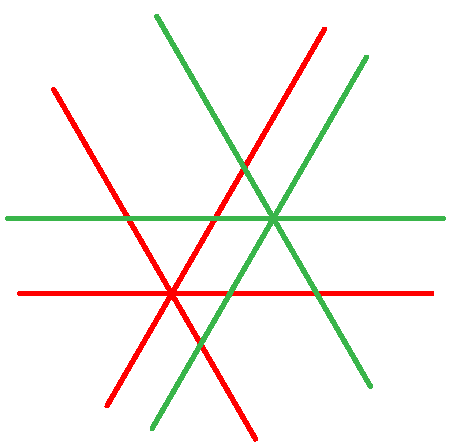
\includegraphics[scale=.4]{multiBraidArrangement2}
		&
		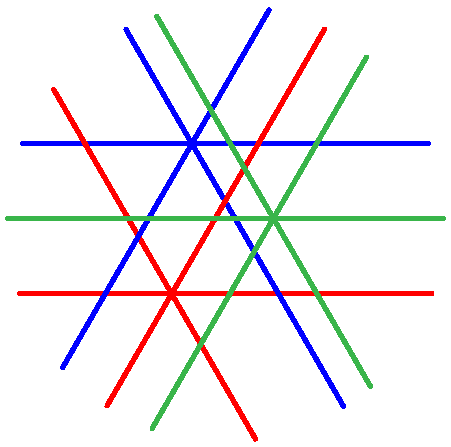
\includegraphics[scale=.4]{multiBraidArrangement3}
		&
		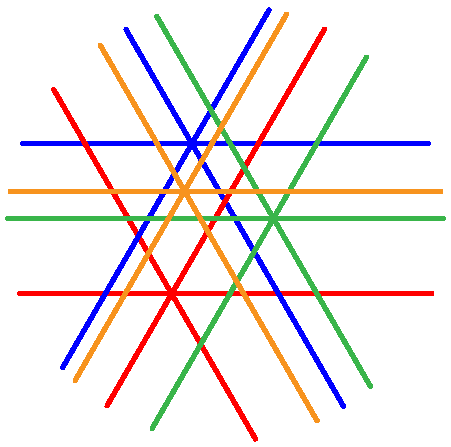
\includegraphics[scale=.4]{multiBraidArrangement4}
		\\
		$\ell = 1$ & $\ell = 2$ & $\ell = 3$ & $\ell = 4$
	\end{tabular}
	}
	\caption{The $(\ell,3)$-braid arrangements for~$\ell \in [4]$.}
	\label{fig:multiBraidArrangements}
\end{figure}

\begin{definition}
For any integers~$\ell,n \geq 1$, the \defn{$(\ell,n)$-braid arrangement}~$\multiBraidArrangement$ is the arrangement obtained as the union of $\ell$ generically translated copies of the braid arrangement~$\braidArrangement$.
\end{definition}

\begin{remark}
\label{rem:multiBraidArrangement}
In practice, consider the hyperplanes~$\set{\b{x} \in \HH}{x_r - x_s = A_{i,r,s}}$ for all~$1 \le r < s \le n$ and~$i \in [\ell]$, where $A_{i,r,s} \eqdef \smash{\sum_{r \le j < s} a_{i,j}}$ for an arbitrary generic matrix~$(a_{i,j}) \in M_{\ell,n-1}(\R)$.
\end{remark}

\begin{definition}
The \defn{intersection hypergraph} of a $\ell$-tuple~$\b{F} \eqdef (F_1, \dots, F_\ell)$ of set partitions of~$[n]$ is the $\ell$-regular $\ell$-partite hypergraph on all parts of all the partitions~$F_i$ for~${i \in [\ell]}$, with an hyperedge connecting the parts containing~$j$  for each~$j \in [n]$.
A \defn{$(\ell,n)$-partition forest} (resp.~\defn{$(\ell,n)$-partition tree}) is a $\ell$-tuple~$\b{F} \eqdef (F_1, \dots, F_\ell)$ of set partitions of~$[n]$ whose intersection hypergraph is a hyperforest (resp.~hypertree).
The \defn{dimension} of~$\b{F}$ is~$\smash{{\dim(\b{F}) \eqdef n - 1 - \ell n + \sum_{i \in [\ell]} \#F_i}}$.
See \cref{fig:forests}.
The \defn{$(\ell,n)$-partition forest poset} is the poset~$\forestPoset$ on $(\ell,n)$-partition forests ordered by componentwise refinement.
In other words, $\forestPoset$ is the subposet of the $\ell$\ordinal{} Cartesian power of the partition poset~$\partitionPoset$ induced by $(\ell,n)$-partition forests.
Note that the maximal elements of~$\forestPoset$ are the $(\ell, n)$-partition trees.
%
\begin{figure}
	\centerline{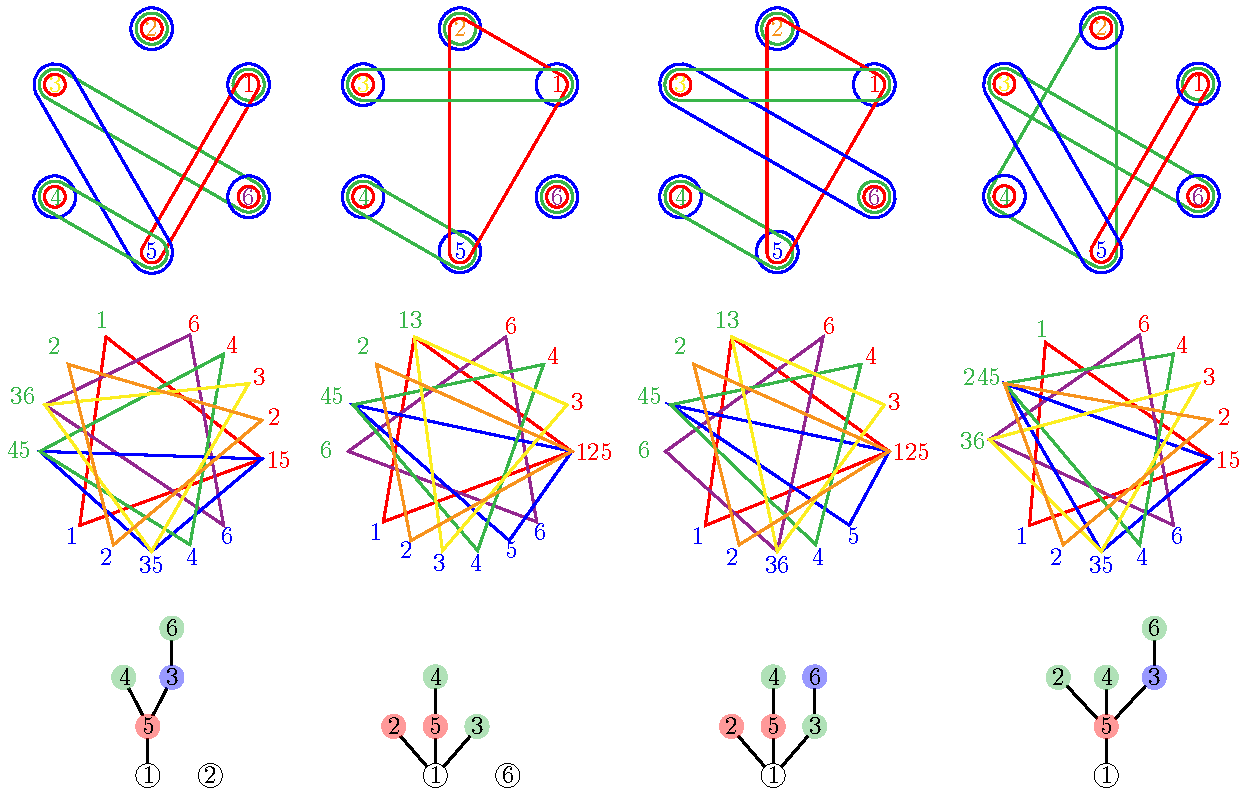
\includegraphics[scale=.9]{forests}}
	\caption{Some $(3,6)$-partition forests (top) with their intersection hypergraphs (middle) and the corresponding labeled $(3,6)$-rainbow forests (bottom). The last two are trees. The order of the colors is red, green, blue.}
	\label{fig:forests}
\end{figure}
\end{definition}

The following statement is illustrated in \cref{fig:intersectionPosetMultiBraidArrangement32}.
%
\begin{figure}
	\centerline{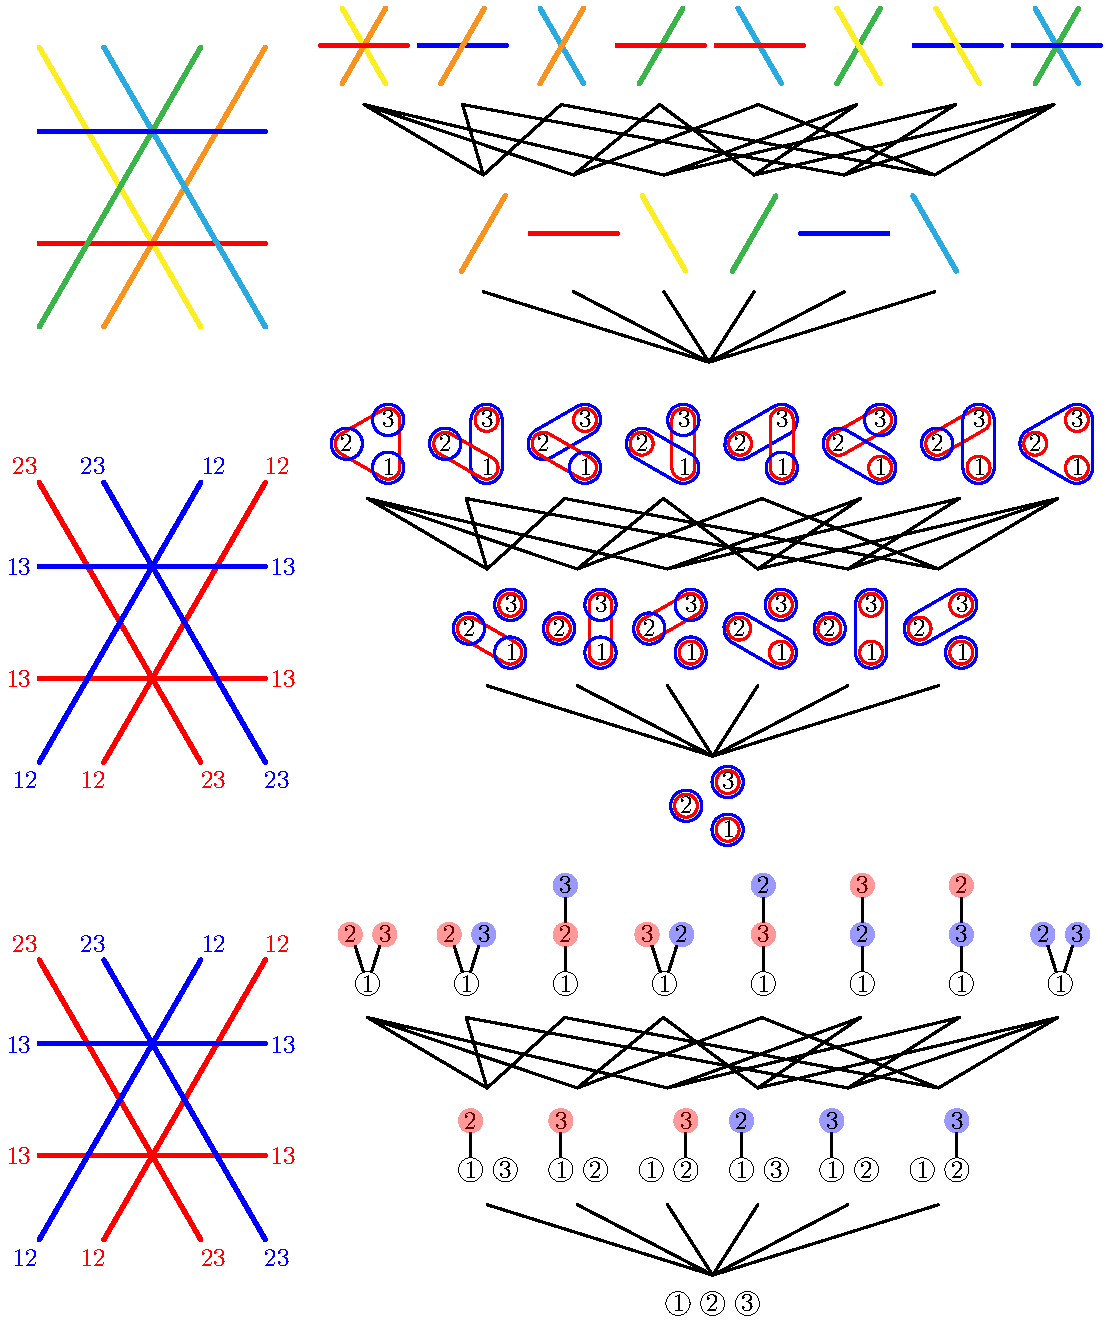
\includegraphics[scale=.9]{figures/intersectionPosetMultiBraidArrangement32Full}}
	\caption{The $(2,3)$-braid arrangement $\multiBraidArrangement[3][2]$ (left), and its flat poset (right), where flats are represented as intersections of hyperplanes (top), as $(2,3)$-partitions forests (middle), and as labeled $(2,3)$-rainbow forests (bottom).}
	\label{fig:intersectionPosetMultiBraidArrangement32}
\end{figure}

\begin{proposition}
\label{prop:flatPosetMultiBraidArrangement}
The flat poset of the $(\ell,n)$-braid arrangement~$\multiBraidArrangement$ is isomorphic to the $(\ell,n)$-partition forest poset.
\end{proposition}

\begin{proof}
Consider the hyperplanes~$\set{\b{x} \in \HH}{x_r - x_s = A_{i,r,s}}$ described in \cref{rem:multiBraidArrangement}.
For each~${i \in [\ell]}$, each set partition~$\pi$ of~$[n]$ corresponds to a $\#\pi$-dimensional flat
\[
\Psi_i(\pi) \eqdef \set{\b{x} \in \HH}{x_r - x_s = A_{i,r,s} \text{ for all } r,s \in p \in F_i }
\]
of the $i$\ordinal{} copy of the braid arrangement~$\braidArrangement$.
The flats of the $(\ell,n)$-braid arrangement~$\multiBraidArrangement$ are thus all of the form
\[
\Psi(\b{F}) \eqdef \bigcap_{i \in [\ell]} \Psi_i(F_i)
\]
for certain $\ell$-tuples~$\b{F} \eqdef (F_1, \dots, F_\ell)$ of set partitions of~$[n]$.
Since the parameters~$A_{i,r,s}$ are generic, $\Psi(\b{F})$ is non-empty if and only if the intersection hypergraph of~$\b{F}$ is acyclic.
Moreover, $\Psi(\b{F})$ is included in~$\Psi(\b{G})$ if and only if~$\b{F}$ refines~$\b{G}$ componentwise.
Hence, the flat poset of~$\multiBraidArrangement$ is isomorphic to the $(\ell,n)$-partition forest poset.
Finally, notice that the codimension of the flat~$\Psi(\b{F})$ is the sum of the codimensions of the flats~$\Psi_i(F_i)$ for~$i \in [\ell]$, so that~$\dim(\b{F}) \eqdef n - 1 - \ell n + \sum_{i \in [\ell]} \#F_i $ is indeed the dimension of the flat~$\Psi(\b{F})$.
\end{proof}

We thus derive the M\"obius polynomial of the $(\ell,n)$-braid arrangement~$\multiBraidArrangement$ by \cref{def:MobiusPolynomial,prop:flatPosetMultiBraidArrangement}.

\begin{theorem}
\label{thm:MobiusPolynomialMultiBraidArrangement}
The M\"obius polynomial of the $(\ell,n)$-braid arrangement~$\multiBraidArrangement$ is given by
\[
\mobPol[\multiBraidArrangement] = x^{n-1-\ell n} y^{n-1-\ell n} \sum_{\b{F} \le \b{G}} \prod_{i \in [\ell]} x^{\#F_i} y^{\#G_i} \prod_{p \in G_i} (-1)^{\#F_i[p]-1} (\# F_i[p]-1)! \; ,
\]
where~$\b{F} \le \b{G}$ ranges over all intervals of the $(\ell,n)$-partition forest poset~$\forestPoset$, and~$F_i[p]$ denotes the restriction of the partition~$F_i$ to the part~$p$ of~$G_i$.
\end{theorem}

\begin{proof}
Observe that for~$\b{F} \eqdef (F_1, \dots, F_\ell)$ and~$\b{G} \eqdef (G_1, \dots, G_\ell)$ in~$\forestPoset$, we have
\[
[\b{F}, \b{G}] = \prod_{i \in [\ell]} [F_i, G_i] \simeq \prod_{i \in [\ell]} \prod_{p \in G_i} \partitionPoset[{\#F_i[p]}].
\]
Recall that the M\"obius function is multiplicative:
\(
\mu_{P \times Q} \big( (p,q), (p’,q’) \big) = \mu_P(p,p’) \cdot \mu_Q(q,q’),
\)
for all~$p, p' \in P$ and~$q, q' \in Q$.
Hence, we obtain that
\[
\mu_{\forestPoset}(\b{F}, \b{G}) = \prod_{i \in [\ell]} \prod_{p \in G_i} (-1)^{\#F_i[p]-1} (\# F_i[p]-1)! \, .
\]
Hence, we derive from \cref{def:MobiusPolynomial,prop:flatPosetMultiBraidArrangement} that
\begin{align*}
\mobPol[\multiBraidArrangement] 
& = \sum_{\b{F} \le \b{G}} \mu_{\forestPoset}(\b{F}, \b{G}) \, x^{\dim(\b{F})} \, y^{\dim(\b{G})} \\
& = x^{n-1-\ell n} y^{n-1-\ell n} \sum_{\b{F} \le \b{G}} \prod_{i \in [\ell]} x^{\#F_i} y^{\#G_i} \prod_{p \in G_i} (-1)^{\#F_i[p]-1} (\# F_i[p]-1)! \, .
\qedhere
\end{align*}
\end{proof}

From \cref{thm:Zaslavsky,thm:MobiusPolynomialMultiBraidArrangement}, we thus obtain the face numbers and bounded face numbers of~$\multiBraidArrangement$, whose first few values are gathered in \cref{table:fvectorMultiBraidArrangements}.

%\begin{table}
%\centerline{
%	\begin{tabular}{c@{\hspace{.7cm}}c}
%		\begin{tabular}[t]{c|cccc|c}
%			$n \backslash k$ & $0$ & $1$ & $2$ & $3$ & $\Sigma$ \\
%			\hline
%			$1$ & $1$ &&&& $1$ \\
%			$2$ & $2$ & $1$ &&& $3$ \\
%			$3$ & $6$ & $6$ & $1$ && $13$ \\
%			$4$ & $24$ & $36$ & $14$ & $1$ & $75$
%		\end{tabular}
%		&
%		\begin{tabular}[t]{c|cccc|c}
%			$n \backslash k$ & $0$ & $1$ & $2$ & $3$ & $\Sigma$ \\
%			\hline
%			$1$ & $1$ &&&& $1$ \\
%			$2$ & $3$ & $2$ &&& $5$ \\
%			$3$ & $17$ & $24$ & $8$ && $49$ \\
%			$4$ & $149$ & $324$ & $226$ & $50$ & $749$
%		\end{tabular}
%		\\[2cm]
%		\begin{tabular}[t]{c|cccc|c}
%			$n \backslash k$ & $0$ & $1$ & $2$ & $3$ & $\Sigma$ \\
%			\hline
%			$1$ & $1$ &&&& $1$ \\
%			$2$ & $0$ & $1$ &&& $1$ \\
%			$3$ & $0$ & $0$ & $1$ && $1$ \\
%			$4$ & $0$ & $0$ & $0$ & $1$ & $1$
%		\end{tabular}
%		&
%		\begin{tabular}[t]{c|cccc|c}
%			$n \backslash k$ & $0$ & $1$ & $2$ & $3$ & $\Sigma$ \\
%			\hline
%			$1$ & $1$ &&&& $1$ \\
%			$2$ & $1$ & $2$ &&& $3$ \\
%			$3$ & $5$ & $12$ & $8$ && $25$ \\
%			$4$ & $43$ & $132$ & $138$ & $50$ & $363$
%		\end{tabular}
%		\\[2cm]
%		$\ell = 1$ & $\ell = 2$
%		\\[.8cm]
%		\begin{tabular}[t]{c|cccc|c}
%			$n \backslash k$ & $0$ & $1$ & $2$ & $3$ & $\Sigma$ \\
%			\hline
%			$1$ & $1$ &&&& $1$ \\
%			$2$ & $4$ & $3$ &&& $7$ \\
%			$3$ & $34$ & $54$ & $21$ && $109$ \\
%			$4$ & $472$ & $1152$ & $924$ & $243$ & $2791$
%		\end{tabular}
%		&
%		\begin{tabular}[t]{c|cccc|c}
%			$n \backslash k$ & $0$ & $1$ & $2$ & $3$ & $\Sigma$ \\
%			\hline
%			$1$ & $1$ &&&& $1$ \\
%			$2$ & $5$ & $4$ &&& $9$ \\
%			$3$ & $57$ & $96$ & $40$ && $193$ \\
%			$4$ & $1089$ & $2808$ & $2396$ & $676$ & $6969$
%		\end{tabular}
%		\\[2cm]
%		\begin{tabular}[t]{c|cccc|c}
%			$n \backslash k$ & $0$ & $1$ & $2$ & $3$ & $\Sigma$ \\
%			\hline
%			$1$ & $1$ &&&& $1$ \\
%			$2$ & $2$ & $3$ &&& $5$ \\
%			$3$ & $16$ & $36$ & $21$ && $73$ \\
%			$4$ & $224$ & $684$ & $702$ & $243$ & $1853$
%		\end{tabular}
%		&
%		\begin{tabular}[t]{c|cccc|c}
%			$n \backslash k$ & $0$ & $1$ & $2$ & $3$ & $\Sigma$ \\
%			\hline
%			$1$ & $1$ &&&& $1$ \\
%			$2$ & $3$ & $4$ &&& $7$ \\
%			$3$ & $33$ & $72$ & $40$ && $145$ \\
%			$4$ & $639$ & $1944$ & $1980$ & $676$ & $5239$
%		\end{tabular}
%		\\[2cm]
%		$\ell = 3$ & $\ell = 4$
%	\end{tabular}
%	}
%	\vspace{.3cm}
%	\caption{The face numbers (top) and the bounded face numbers (bottom) of the $(\ell,n)$-braid arrangements for~$\ell, n \in [4]$.}
%	\label{table:fvectorMultiBraidArrangements}
%\end{table}

\begin{table}
	\centerline{\scalebox{.8}{
		\begin{tabular}{c@{\hspace{.7cm}}c@{\hspace{.7cm}}c@{\hspace{.7cm}}c}
			$\ell = 1$ & $\ell = 2$ & $\ell = 3$ & $\ell = 4$
			\\[.2cm]
			\begin{tabular}[t]{c|cccc|c}
				$n \backslash k$ & $0$ & $1$ & $2$ & $3$ & $\Sigma$ \\
				\hline
				$1$ & $1$ &&&& $1$ \\
				$2$ & $2$ & $1$ &&& $3$ \\
				$3$ & $6$ & $6$ & $1$ && $13$ \\
				$4$ & $24$ & $36$ & $14$ & $1$ & $75$
			\end{tabular}
			&
			\begin{tabular}[t]{c|cccc|c}
				$n \backslash k$ & $0$ & $1$ & $2$ & $3$ & $\Sigma$ \\
				\hline
				$1$ & $1$ &&&& $1$ \\
				$2$ & $3$ & $2$ &&& $5$ \\
				$3$ & $17$ & $24$ & $8$ && $49$ \\
				$4$ & $149$ & $324$ & $226$ & $50$ & $749$
			\end{tabular}
			&
			\begin{tabular}[t]{c|cccc|c}
				$n \backslash k$ & $0$ & $1$ & $2$ & $3$ & $\Sigma$ \\
				\hline
				$1$ & $1$ &&&& $1$ \\
				$2$ & $4$ & $3$ &&& $7$ \\
				$3$ & $34$ & $54$ & $21$ && $109$ \\
				$4$ & $472$ & $1152$ & $924$ & $243$ & $2791$
			\end{tabular}
			&
			\begin{tabular}[t]{c|cccc|c}
				$n \backslash k$ & $0$ & $1$ & $2$ & $3$ & $\Sigma$ \\
				\hline
				$1$ & $1$ &&&& $1$ \\
				$2$ & $5$ & $4$ &&& $9$ \\
				$3$ & $57$ & $96$ & $40$ && $193$ \\
				$4$ & $1089$ & $2808$ & $2396$ & $676$ & $6969$
			\end{tabular}
			\\[2.3cm]
			\begin{tabular}[t]{c|cccc|c}
				$n \backslash k$ & $0$ & $1$ & $2$ & $3$ & $\Sigma$ \\
				\hline
				$1$ & $1$ &&&& $1$ \\
				$2$ & $0$ & $1$ &&& $1$ \\
				$3$ & $0$ & $0$ & $1$ && $1$ \\
				$4$ & $0$ & $0$ & $0$ & $1$ & $1$
			\end{tabular}
			&
			\begin{tabular}[t]{c|cccc|c}
				$n \backslash k$ & $0$ & $1$ & $2$ & $3$ & $\Sigma$ \\
				\hline
				$1$ & $1$ &&&& $1$ \\
				$2$ & $1$ & $2$ &&& $3$ \\
				$3$ & $5$ & $12$ & $8$ && $25$ \\
				$4$ & $43$ & $132$ & $138$ & $50$ & $363$
			\end{tabular}
			&
			\begin{tabular}[t]{c|cccc|c}
				$n \backslash k$ & $0$ & $1$ & $2$ & $3$ & $\Sigma$ \\
				\hline
				$1$ & $1$ &&&& $1$ \\
				$2$ & $2$ & $3$ &&& $5$ \\
				$3$ & $16$ & $36$ & $21$ && $73$ \\
				$4$ & $224$ & $684$ & $702$ & $243$ & $1853$
			\end{tabular}
			&
			\begin{tabular}[t]{c|cccc|c}
				$n \backslash k$ & $0$ & $1$ & $2$ & $3$ & $\Sigma$ \\
				\hline
				$1$ & $1$ &&&& $1$ \\
				$2$ & $3$ & $4$ &&& $7$ \\
				$3$ & $33$ & $72$ & $40$ && $145$ \\
				$4$ & $639$ & $1944$ & $1980$ & $676$ & $5239$
			\end{tabular}
		\end{tabular}
	}}
	\vspace{.3cm}
	\caption{The face numbers (top) and the bounded face numbers (bottom) of the $(\ell,n)$-braid arrangements for~$\ell, n \in [4]$.}
	\label{table:fvectorMultiBraidArrangements}
\end{table}

\begin{corollary}
\label{coro:fbvectorsMultiBraidArrangement}
The $f$- and $b$-polynomials of the $(\ell,n)$-braid arrangement~$\multiBraidArrangement$ are given by
\begin{align*}
\fPol[\multiBraidArrangement] & = x^{n-1-\ell n}\sum_{\b{F} \le \b{G}} \prod_{i \in [\ell]} x^{\#F_i} \prod_{p \in G_i} (\# F_i[p]-1)!\\
\text{and}\qquad
\bPol[\multiBraidArrangement] & = (-1)^\ell x^{n-1-\ell n} \sum_{\b{F} \le \b{G}} \prod_{i \in [\ell]} x^{\#F_i} \prod_{p \in G_i} -(\# F_i[p]-1)! \, ,
\end{align*}
where~$\b{F} \le \b{G}$ ranges over all intervals of the $(\ell,n)$-partition forest poset~$\forestPoset$, and~$F_i[p]$ denotes the restriction of the partition~$F_i$ to the part~$p$ of~$G_i$.
\end{corollary}

\begin{example}
For~$n = 1$, we have
\[
\mobPol[{\multiBraidArrangement[1][\ell]}] = \fPol[{\multiBraidArrangement[1][\ell]}] = \bPol[{\multiBraidArrangement[1][\ell]}] = 1.
\]
For~$n = 2$, we have
\[
\mobPol[{\multiBraidArrangement[2][\ell]}] = xy-\ell x+\ell,
\quad
\fPol[{\multiBraidArrangement[2][\ell]}] = (\ell+1)x+\ell
\quad\text{and}\quad
\bPol[{\multiBraidArrangement[2][\ell]}] = (\ell-1)x+\ell.
\]
The case~$n = 3$ is already more interesting.
Consider the set partitions~$P \eqdef \big\{ \{1\}, \{2\}, \{3\} \big\}$, $Q_i \eqdef \big\{ \{i\}, [3] \ssm \{i\} \big\}$ for~$i \in [3]$, and~$R \eqdef \big\{ [3] \big\}$.
Observe that the $(\ell,3)$-partition forests are all of the form
\begin{gather*}
\b{F} \eqdef P^\ell,
\quad
\b{G}_i^p \eqdef P^p Q_i P^{\ell-p-1}, % \text{ for } p \le \ell-1 \text{ and } i \in [3],
\quad
\b{H}_{i,j}^{p,q} \eqdef P^p Q_i P^{\ell-p-q-2} Q_j P^q \;\text{($i \ne j$)} % \text{ for } p + q \le \ell-2 \text{ and } i \ne j \in [3]
\quad\text{or}\quad
\b{K}^p \eqdef P^p R P^{\ell-p-1}. % \text{ for } p \le \ell-1.
\end{gather*}
(where we write a tuple of partitions of~$[3]$ as a word on~$\{P, Q_1, Q_2, Q_3, R\}$, and $p$ and $q$ are such that the total length is~$\ell$).
%\begin{gather*}
%\b{F} \eqdef (\underbrace{P, \dots, P}_\ell), \\
%\b{G}_i^p \eqdef (\underbrace{P, \dots, P}_p, Q_i, \underbrace{P, \dots, P}_{\ell-p-1}) \text{ for } p \le \ell-1 \text{ and } i \in [3],
%\\
%\b{H}_{i,j}^{p,q} \eqdef (\underbrace{P, \dots, P}_p, Q_i, \underbrace{P, \dots, P}_{\ell-p-q-2}, Q_j, \underbrace{P, \dots, P}_q) \text{ for } p + q \le \ell-2 \text{ and } i \ne j \in [3],
%\\
%\text{or}\quad
%\b{K}^p \eqdef (\underbrace{P, \dots, P}_p, R, \underbrace{P, \dots, P}_{\ell-p-1}) \text{ for } p \le \ell-1.
%\end{gather*}
Moreover, the cover relations in the $(\ell,3)$-partition forest poset are precisely the relations
\[
\b{F} \le \b{G}_i^p \hspace{-.4cm} \begin{array}{l} \rotatebox[origin=c]{45}{$\le$} \raisebox{.2cm}{$\b{H}_{i,j}^{p,q}$} \\[.1cm] \quad \le \b{K}^p \\[.1cm] \rotatebox[origin=c]{-45}{$\le$} \raisebox{-.2cm}{$\b{H}_{j,i}^{\ell-q-1, \ell-p-1}$} \end{array}
\]
for~$i \ne j$ and~$p, q$ such that~$p + q \le \ell-2$.
Hence, we have
\begin{align*}
\mobPol[{\multiBraidArrangement[3][\ell]}] & = x^2 y^2 - 3 \ell x^2 y + \ell (3 \ell - 1) x^2 + 3 \ell x y - 3 \ell (2 \ell - 1) x + \ell (3 \ell - 2) , \\
\fPol[{\multiBraidArrangement[3][\ell]}] & = (3 \ell^2 + 2 \ell + 1) x^2 + 6 \ell^2 x + \ell (3 \ell - 2), \\
\text{and}\qquad
\bPol[{\multiBraidArrangement[3][\ell]}] & = (3 \ell^2 - 4 \ell + 1) x^2 + 6 \ell (\ell - 1) x + \ell (3 \ell - 2).
\end{align*}
Observe that~$3 \ell^2 + 2 \ell + 1$ is~\OEIS{A056109}, that~$\ell (3 \ell - 2)$ is~\OEIS{A000567}, and that ${3 \ell^2 - 4 \ell + 1}$ is~\OEIS{A045944}.
\vincenti{There is a weird connection between the first and the last. Namely, $3 \ell^2 - 4 \ell + 1 = 3 (\ell - 1)^2 + 2 (\ell - 1)$. Is there a bijective explanation on the arrangements?}
\end{example}

\begin{remark}
\vincenti{TODO: Discuss generalizations to $\ell$ copies of an arbitrary arrangement, or a graphical arrangement.}
\end{remark}

%%%%%%%%%%%%%%%

\subsection{Rainbow forests}
\label{subsec:rainbowForests}

In order to obtain more explicit formulas for the number of vertices and regions of the $(\ell,n)$-braid arrangement~$\multiBraidArrangement$ in \cref{subsec:verticesFacetsMultiBraidArrangement}, we now introduce another combinatorial model for $(\ell,n)$-partition forests which is more adapted to their enumeration.

\begin{definition}
\label{def:rainbowForest}
A \defn{$\ell$-rainbow coloring} of a rooted plane forest~$F$ is an assignment of colors of~$[\ell]$ to the non-root nodes of~$F$ such that
\begin{enumerate}[(i)]
\item there is no monochromatic edge,
\item the colors of siblings are increasing from left to right.
\end{enumerate}
We denote by~$\|F\|$ the number of nodes of~$F$ and by~$\#F$ the number of trees of the forest~$F$ (\ie its number of connected components).
A \defn{$(\ell,n)$-rainbow forest} (resp.~\defn{tree}) is a \mbox{$\ell$-rainbow} colored forest (resp.~tree) with $\|F\| = n$ nodes.
We denote by~$\rainbowForests$ (resp.~$\rainbowTrees$) the set of $(\ell,n)$-rainbow forests (resp.~trees), and set~$\rainbowForests[][\ell] \eqdef \bigsqcup_n \rainbowForests$ (resp.~$\rainbowTrees[][\ell] \eqdef \bigsqcup_n \rainbowTrees$).
\end{definition}

For instance, we have listed all $(2,4)$-rainbow trees in \cref{fig:rainbowTrees}\,(top).
This figure actually illustrates the following statement.

\begin{lemma}
\label{lem:FussCatalan}
The $(\ell,m)$-rainbow trees are counted by the \defn{Fuss-Catalan number}
\[
\# \rainbowTrees[m][\ell] = F_{\ell,m} \eqdef \frac{1}{(\ell-1)m+1} \binom{\ell m}{m} \qquad \text{\OEIS{A062993}}.
\]
\end{lemma}

\begin{proof}
We can transform a $\ell$-rainbow tree~$R$ to a $\ell$-ary tree~$T$ as illustrated in \cref{fig:rainbowTrees}.
Namely, the parent of a node~$N$ in~$T$ is the previous sibling colored as~$N$ in~$R$ if it exists, and the parent of~$N$ in~$R$ otherwise.
This classical map is a bijection from $\ell$-rainbow trees to a $\ell$-ary trees, which are counted by the Fuss-Catalan numbers~\cite{Klarner, HiltonPedersen}.
\vincent{not sure of the attribution...}
%
\begin{figure}
	\centerline{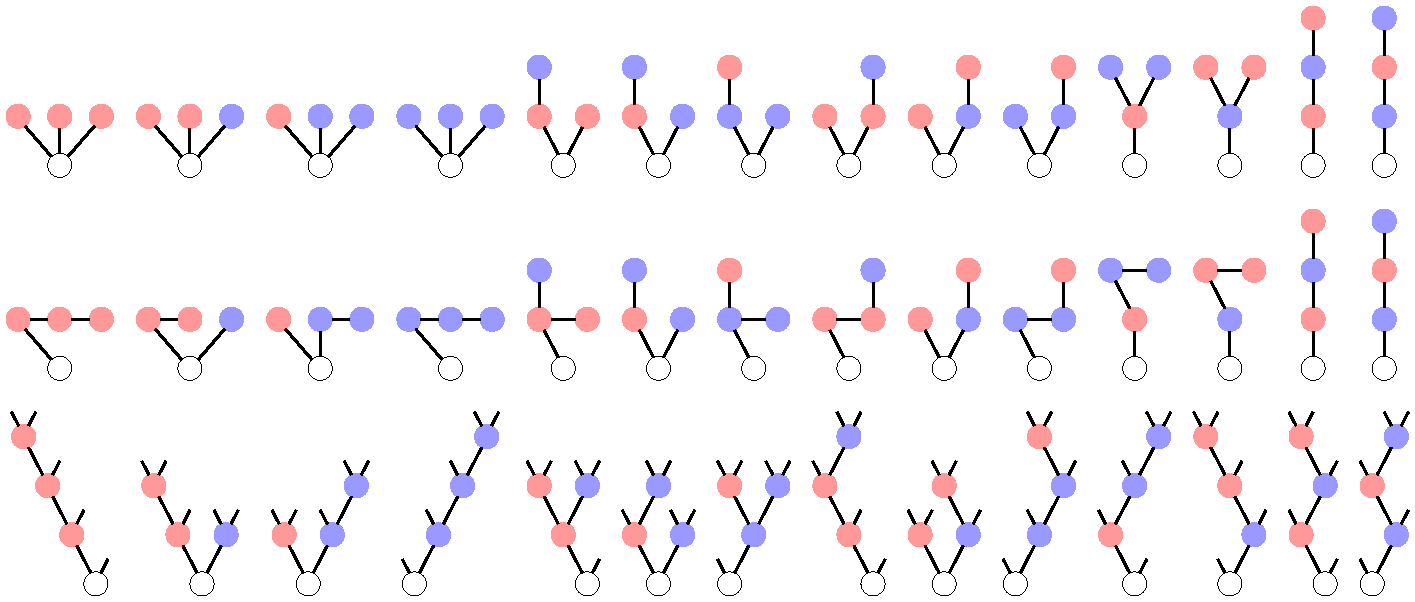
\includegraphics[scale=.7]{rainbowTrees}}
	\caption{The $14$ $(2,4)$-rainbow trees (top) and $14$ binary trees (bottom), and the simple bijection between them (middle). The order of the colors is red, blue.}
	\label{fig:rainbowTrees}
\end{figure}
\end{proof}

\begin{remark}
\label{rem:functionalEquationFussCatalan}
Recall that the corresponding generating function~$F_\ell(z) \eqdef \sum_{m \ge 0} F_{\ell,m} \, z^m$ satisfies the functional equiation
\[
F_\ell(z) = 1 + z \, F_\ell(z)^\ell.
\]
\end{remark}

\begin{table}
	\centerline{\scalebox{.8}{
		\begin{tabular}[t]{c|ccccccccc}
			$m \backslash \ell$ & $1$ & $2$ & $3$ & $4$ & $5$ & $6$ & $7$ & $8$ & $9$ \\
			\hline
			$1$ & $1$ & $1$ & $1$ & $1$ & $1$ & $1$ & $1$ & $1$ & $1$ \\
			$2$ & $1$ & $2$ & $3$ & $4$ & $5$ & $6$ & $7$ & $8$ & $9$ \\
			$3$ & $1$ & $5$ & $12$ & $22$ & $35$ & $51$ & $70$ & $92$ & $117$ \\
			$4$ & $1$ & $14$ & $55$ & $140$ & $285$ & $506$ & $819$ & $1240$ & $1785$ \\
			$5$ & $1$ & $42$ & $273$ & $969$ & $2530$ & $5481$ & $10472$ & $18278$ & $29799$ \\
			$6$ & $1$ & $132$ & $1428$ & $7084$ & $23751$ & $62832$ & $141778$ & $285384$ & $527085$ \\
			$7$ & $1$ & $429$ & $7752$ & $53820$ & $231880$ & $749398$ & $1997688$ & $4638348$ & $9706503$ \\
			$8$ & $1$ & $1430$ & $43263$ & $420732$ & $2330445$ & $9203634$ & $28989675$ & $77652024$ & $184138713$ \\
			$9$ & $1$ & $4862$ & $246675$ & $3362260$ & $23950355$ & $115607310$ & $430321633$ & $1329890705$ & $3573805950$
		\end{tabular}
	}}
	\vspace{.3cm}
	\caption{The Fuss-Catalan numbers~$F_{\ell,m} = \frac{1}{(\ell-1)m+1} \binom{\ell m}{m}$ for~$\ell,m \in [9]$. See \OEIS{A062993}.}
\end{table}

\begin{definition}
For a rainbow forest~$F$, we define
\[
\omega(F) \eqdef \prod_{i \in [\ell]} \prod_{N \in F} \#C_i(N)! \, ,
\]
where~$N$ ranges over all nodes of~$F$ and~$C_i(N)$ denotes the children of~$N$ colored by~$i$.
\end{definition}

\begin{definition}
\label{def:labelingRainbowForest}
A \defn{labeling} of a $(\ell,n)$-rainbow forest~$F$ is a bijective map between from the nodes of~$F$ to~$[n]$ such that
\begin{enumerate}[(i)]
\item the label of each root is minimal in its tree,
\item the labels of siblings with the same color are increasing from left to right.
\end{enumerate}
\end{definition}

\begin{lemma}
\label{lem:labelingRainbowForest}
The number~$\lambda(F)$ of labelings of a $(\ell,n)$-rainbow forest~$F$ is given by
\[
\lambda(F) = \frac{n!}{\omega(F) \prod\limits_{T \in F} \|T\|} \, .
\]
\end{lemma}

\begin{proof}
Out of all~$n!$ bijective maps from the nodes of~$F$ to~$[n]$, only~$1/\prod_{T \in F} \|T\|$ satisfy Condition~(i) of \cref{def:labelingRainbowForest}, and only $1/\prod_{i \in [\ell]} \prod_{N \in F} \#C_i(N)! = 1/\omega(F)$ satisfy Condition~(ii) of \cref{def:labelingRainbowForest}.
\end{proof}

The following statement is illustrated in \cref{fig:forests}.

\begin{proposition}
\label{prop:bijectionForests}
There is a bijection from $(\ell,n)$-partition forests to labeled $(\ell,n)$-rainbow forests, such that if the partition forest~$\b{F}$ is sent to the labeled rainbow forest~$F$, then
\[
\dim(\b{F}) = \#F-1
\qquad\text{and}\qquad
\mu_{\forestPoset}(\HH, \b{F}) = (-1)^{n-\#F} \, \omega(F).
\]
\end{proposition}

\begin{proof}
From a labeled $(\ell,n)$-rainbow forest~$F$, we construct a $(\ell,n)$-partition forest~$\b{F} \eqdef (F_1, \dots, F_\ell)$ whose $i$\ordinal{} partition~$F_i$ has a part~$\{N\} \cup C_i(N)$ for each node~$N$ of~$F$ not colored~$i$.
Condition~(i) of \cref{def:rainbowForest} ensures that each $F_i$ is indeed a partition.

Conversely, start from a $(\ell,n)$-partition forest~$\b{F} \eqdef (F_1, \dots, F_i)$.
Consider the colored clique graph~$K_{\b{F}}$ on~$[n]$ obtained by replacing each part in~$F_i$ by a clique of edges colored by~$i$.
For each~$1 < j \le n$, there is a unique shortest path in~$K_{\b{F}}$ from the vertex~$j$ to the smallest vertex in the connected component of~$j$.
Define the parent~$p$ of~$j$ to be the next vertex along this path, and color the node~$j$ by the color of the edge between~$j$ and~$p$.
This defines a labeled $(\ell,n)$-rainbow forest~$F$.

Finally, observe that
\begin{gather*}
\dim(\b{F}) = n - 1 - \ell n + \sum_{i \in [\ell]} \#F_i = \#F-1, \qquad\text{and} \\
\mu_{\forestPoset}(\HH, \b{F}) = \prod\limits_{i \in [\ell]} \prod\limits_{p \in F_i} (-1)^{\#p-1} (\#p-1) = \prod\limits_{i \in [\ell]} \prod\limits_{N \in F} (-1)^{\#C_i(N)} \#C_i(N)! = (-1)^{n-\#F} \, \omega(F).
\qedhere
\end{gather*}
\end{proof}

%%%%%%%%%%%%%%%

\subsection{Enumeration of vertices and regions of $\multiBraidArrangement$}
\label{subsec:verticesFacetsMultiBraidArrangement}

We now use the labeled $(\ell,n)$-rainbow forests of \cref{subsec:rainbowForests} to derive more explicit formulas for the number of vertices and regions of the $(\ell,n)$-braid arrangement~$\multiBraidArrangement$.
We start with the number of vertices of~$\multiBraidArrangement$, whose first values are gathered in \cref{table:verticesMultiBraidArrangement}.

\begin{table}
	\centerline{\scalebox{.8}{
		\begin{tabular}[t]{c|cccccccc}
			$n \backslash \ell$ & $1$ & $2$ & $3$ & $4$ & $5$ & $6$ & $7$ & $8$ \\ % & $9$ \\
			\hline
		$1$ & $1$ & $1$ & $1$ & $1$ & $1$ & $1$ & $1$ & $1$ \\ % & $1$ \\
		$2$ & $1$ & $2$ & $3$ & $4$ & $5$ & $6$ & $7$ & $8$ \\ % & $9$ \\
		$3$ & $1$ & $8$ & $21$ & $40$ & $65$ & $96$ & $133$ & $176$ \\ % & $225$ \\
		$4$ & $1$ & $50$ & $243$ & $676$ & $1445$ & $2646$ & $4375$ & $6728$ \\ % & $9801$ \\
		$5$ & $1$ & $432$ & $3993$ & $16384$ & $46305$ & $105456$ & $208537$ & $373248$ \\ % & $620289$ \\
		$6$ & $1$ & $4802$ & $85683$ & $521284$ & $1953125$ & $5541126$ & $13119127$ & $27350408$ \\ % & $51883209$ \\
		$7$ & $1$ & $65536$ & $2278125$ & $20614528$ & $102555745$ & $362797056$ & $1029059101$ & $2500000000$ \\ % & $5415228513$ \\
		$8$ & $1$ & $1062882$ & $72412707$ & $976562500$ & $6457339845$ & $28500625446$ & $96889010407$ & $274371577992$ \\ % & $678770015625$ \\
%		$9$ & $1$ & $20000000$ & $2681615217$ & $53971714048$ & $474659385665$ & $2614905943296$ & $10657046640625$ & $35184372088832$ & $99426586671873$
		\end{tabular}
	}}
	\vspace{.3cm}
	\caption{The numbers $f_0(\multiBraidArrangement) = \ell \big( (\ell-1) n + 1 \big)^{n-2}$ of vertices of~$\multiBraidArrangement$ for~$\ell,n \in [8]$.}
	\label{table:verticesMultiBraidArrangement}
\end{table}

\begin{theorem}
\label{thm:verticesMultiBraidArrangement}
The number of vertices of the $(\ell,n)$-braid arrangement~$\multiBraidArrangement$ is
\[
f_0(\multiBraidArrangement) = \ell \big( (\ell-1) n + 1 \big)^{n-2}.
\]
\end{theorem}

\begin{proof}
By \cref{prop:flatPosetMultiBraidArrangement,prop:bijectionForests}, we just need to count the labeled $(\ell,n)$-rainbow trees.
A common reasoning for counting Cayley trees is the use of its Prüfer code defined by recursively pruning the smallest leaf while writing down the label of its parent.
This bijection can be adapted to colored Cayley trees by writing down the label of the parent colored by the color of the pruned leaf.
This leads to a bijection with certain colored words of length $n-1$.
Namely, there are two possibilities:
\begin{itemize}
\item either the pruned leaf is attached to the node~$1$ and it can have all $\ell$ colors,
\item or it is attached to one of the $n-1$ other nodes and it can only have $\ell-1$ colors.
\end{itemize}
Note that the last letter in the Prüfer code (obtained by removing the last edge) is necessarily the root $1$, with $\ell$ possible different colors.
Hence, there are 
\[
\big( \ell+(n-1)(\ell-1) \big)^{n-2} \ell = \ell \big( (\ell-1) n + 1 \big)^{n-2}
\]
such words.
Similar ideas where used in~\cite{Lewis}.
\vincent{Improve citation?}
\end{proof}

\begin{theorem}
\label{thm:verticesRefinedMultiBraidArrangement}
For any~$k_1, \dots, k_\ell$ such that~$0 \le k_i \le n-1$ for~$i \in [\ell]$ and~${\sum_{i=1}^\ell k_i = n-1}$, the number of vertices~$v$ of the $(\ell,n)$-braid arrangement~$\multiBraidArrangement$ such that the smallest flat of the $i$\ordinal{} copy of~$\braidArrangement$ containing~$v$ has dimension~$n-k_i-1$ is given by
\[
n^{\ell-1} \binom{n-1}{k_1, \dots, k_\ell} \prod_{i=1}^\ell (n-k_i)^{k_i-1}.
\]
\end{theorem}

\begin{proof}
By \cref{prop:flatPosetMultiBraidArrangement,prop:bijectionForests}, we just need to count the labeled $(\ell,n)$-rainbow trees with~$k_i$ nodes colored by~$i$.
Forgetting the labels, the $(\ell,n)$-rainbow trees with~$k_i$ nodes colored by~$i$ are precisely the spanning trees of the complete multipartite graph~$K_{k_1, \dots, k_\ell, 1}$ (where the last~$1$ stands for the uncolored root).
Using a Pr\"ufer code similar to that of the proof of \cref{thm:verticesMultiBraidArrangement}, R.~Lewis proved in~\cite{Lewis} that the latter are counted by~${n^{\ell-1} \prod_{i=1}^\ell (n-k_i)^{k_i-1}}$.
Finally, the possible labelings are counted by the multinomial coefficient~$\binom{n-1}{k_1, \dots, k_\ell}$.
\end{proof}

\begin{theorem}
\label{thm:topCoefficientMobiusPolynomialMultiBraidArrangement}
The characteristic polynomial~$\charPol[\multiBraidArrangement]$ of the $(\ell,n)$-braid arrangement~$\multiBraidArrangement$ is given~by
\[
\charPol[\multiBraidArrangement] = \frac{(-1)^n n!}{y} \, [z^n] \, \exp \bigg( - \sum_{m \ge 1} \frac{F_{\ell,m} \, y \, z^m}{m} \bigg) ,
\]
where~$\displaystyle F_{\ell,m} \eqdef \frac{1}{(\ell-1)m+1} \binom{\ell m}{m}$ is the Fuss-Catalan number.
\end{theorem}

\begin{proof}
By \cref{thm:MobiusPolynomialMultiBraidArrangement,prop:bijectionForests}, the characteristic polynomial~$\charPol[\multiBraidArrangement]$ is
\[
\charPol[\multiBraidArrangement] = \sum_{\b{F} \in \forestPoset} \mu_{\forestPoset}(\HH, \b{F}) \, y^{\dim(\b{F})} = \sum_{F \in \rainbowForests} \lambda(F) \, (-1)^{n-\#F} \, \omega(F) \, y^{\#F-1}.
\]
From \cref{lem:labelingRainbowForest}, we observe that
\[
\frac{\lambda(F) \, \omega(F) \, (-y)^{\#F} \, z^{\|F\|}}{\|F\|!} = \prod_{T \in F} \frac{-y \, z^{\|T\|}}{\|T\|} \, ,
\]
where $T$ ranges over the trees of~$F$.
Now using that rainbow forests are exactly sets of rainbow trees, we obtain that
\[
\sum_{F \in \rainbowForests[][\ell]} \frac{ \lambda(F) \, \omega(F) \, (-y)^{\#F} \, z^{\|F\|}}{\|F\|!} = \sum_{F \in \rainbowForests[][\ell]} \prod_{T \in F} \frac{-y \, z^{\|T\|}}{\|T\|} = \exp \bigg( \sum_{T \in \rainbowTrees[][\ell]} \frac{-y \, z^{\|T\|}}{\|T\|} \bigg).
\]
From \cref{lem:FussCatalan}, we obtain that
\[
\exp \bigg( \sum_{T \in \rainbowTrees[][\ell]} \frac{-y \, z^{\|T\|}}{\|T\|} \bigg) = \exp \bigg( - \sum_{m \ge 1} \frac{F_{\ell,m} \, y \, z^m}{m} \bigg).
\]
We conclude that
\begin{align*}
\charPol[\multiBraidArrangement] 
& = \sum_{F \in \rainbowForests}  \lambda(F) \, (-1)^{n-\#F} \, \omega(F) \, y^{\#F-1} \\
& = \frac{(-1)^n \, n!}{y} [z^n] \sum_{F \in \rainbowForests[][\ell]} \frac{ \lambda(F) \, \omega(F) \, (-y)^{\#F} \, z^{\|F\|}}{\|F\|!} \\
& = \frac{(-1)^n n!}{y} \, [z^n] \, \exp \bigg( - \sum_{m \ge 1} \frac{F_{\ell,m} \, y \, z^m}{m} \bigg).
\qedhere
\end{align*}
\end{proof}

By \cref{rem:characteristicPolynomial,thm:topCoefficientMobiusPolynomialMultiBraidArrangement}, we obtain the number of regions and bounded regions of~$\multiBraidArrangement$, whose first values are gathered in \cref{table:regionsMultiBraidArrangement,table:boundedRegionsMultiBraidArrangement}.

\begin{table}
	\centerline{\scalebox{.8}{
		\begin{tabular}[t]{c|cccccccc}
			$n \backslash \ell$ & $1$ & $2$ & $3$ & $4$ & $5$ & $6$ & $7$ & $8$ \\ % & $9$ \\
			\hline
			$1$ & $1$ & $1$ & $1$ & $1$ & $1$ & $1$ & $1$ & $1$ \\ % & $1$ \\
			$2$ & $2$ & $3$ & $4$ & $5$ & $6$ & $7$ & $8$ & $9$ \\ % & $10$ \\
			$3$ & $6$ & $17$ & $34$ & $57$ & $86$ & $121$ & $162$ & $209$ \\ % & $262$ \\
			$4$ & $24$ & $149$ & $472$ & $1089$ & $2096$ & $3589$ & $5664$ & $8417$ \\ % & $11944$ \\
			$5$ & $120$ & $1809$ & $9328$ & $29937$ & $73896$ & $154465$ & $287904$ & $493473$ \\ % & $793432$ \\
			$6$ & $720$ & $28399$ & $241888$ & $1085157$ & $3442816$ & $8795635$ & $19376064$ & $38323753$ \\ % & $69841072$ \\
			$7$ & $5040$ & $550297$ & $7806832$ & $49075065$ & $200320816$ & $625812385$ & $1629858672$ & $3720648337$ \\ % & $7686190000$ \\
			$8$ & $40320$ & $12732873$ & $302346112$ & $2666534049$ & $14010892416$ & $53536186825$ & $164859458688$ & $434390214657$ \\ % & $1017282905344$ \\
%			$9$ & $362880$ & $343231361$ & $13682809216$ & $169423639713$ & $1146173002496$ & $5357227099105$ & $19506923076096$ & $59328538244801$ & $157507267166848$
		\end{tabular}
	}}
	\vspace{.3cm}
	\caption{The numbers $f_{n-1}(\multiBraidArrangement)$ of regions of~$\multiBraidArrangement$ for~$\ell,n \in [8]$.}
	\label{table:regionsMultiBraidArrangement}
\end{table}

\begin{table}
	\centerline{\scalebox{.8}{
		\begin{tabular}[t]{c|cccccccc}
			$n \backslash \ell$ & $1$ & $2$ & $3$ & $4$ & $5$ & $6$ & $7$ & $8$ \\ % & $9$ \\
			\hline
			$1$ & $1$ & $1$ & $1$ & $1$ & $1$ & $1$ & $1$ & $1$ \\ % & $1$ \\
			$2$ & $0$ & $1$ & $2$ & $3$ & $4$ & $5$ & $6$ & $7$ \\ % & $8$ \\
			$3$ & $0$ & $5$ & $16$ & $33$ & $56$ & $85$ & $120$ & $161$ \\ % & $208$ \\
			$4$ & $0$ & $43$ & $224$ & $639$ & $1384$ & $2555$ & $4248$ & $6559$ \\ % & $9584$ \\
			$5$ & $0$ & $529$ & $4528$ & $17937$ & $49696$ & $111745$ & $219024$ & $389473$ \\ % & $644032$ \\
			$6$ & $0$ & $8501$ & $120272$ & $663363$ & $2354624$ & $6455225$ & $14926176$ & $30583847$ \\ % & $57255488$ \\
			$7$ & $0$ & $169021$ & $3968704$ & $30533409$ & $138995776$ & $464913325$ & $1268796096$ & $2996735329$ \\ % & $6353133184$ \\
			$8$ & $0$ & $4010455$ & $156745472$ & $1684352799$ & $9841053184$ & $40179437975$ & $129465630720$ & $352560518527$ \\ % & $846588258944$ \\
%			$9$ & $0$ & $110676833$ & $7216242688$ & $108413745057$ & $813420601856$ & $4055310777025$ & $15431698810368$ & $48461340225473$ & $131823966149632$
		\end{tabular}
	}}
	\vspace{.3cm}
	\caption{The numbers $b_{n-1}(\multiBraidArrangement)$ of bounded regions of~$\multiBraidArrangement$ for~$\ell,n \in [8]$.}
	\label{table:boundedRegionsMultiBraidArrangement}
\end{table}

\begin{theorem}
\label{thm:regionsMultiBraidArrangement}
The numbers of regions and of bounded regions of the $(\ell,n)$-braid arrangement~$\multiBraidArrangement$ are given by
\begin{align*}
f_{n-1}(\multiBraidArrangement) 
& = n! \, [z^n] \exp \Bigg( \sum_{m \ge 1} \frac{F_{\ell,m} \, z^m}{m} \Bigg) \\
\text{and}\qquad
b_{n-1}(\multiBraidArrangement)
%& = - n! \, [z^n] \exp \Bigg( - \sum_{m \ge 1} \frac{F_{\ell,m} \, z^m}{m} \Bigg) 
& = (n-1)! \, [z^{n-1}] \exp \bigg( (\ell-1) \sum_{m \ge 1} F_{\ell,m} \, z^m \bigg).
\end{align*}
where~$\displaystyle F_{\ell,m} \eqdef \frac{1}{(\ell-1)m+1} \binom{\ell m}{m}$ is the Fuss-Catalan number.
\end{theorem}

\begin{proof}
By \cref{rem:characteristicPolynomial}, we obtain from \cref{thm:topCoefficientMobiusPolynomialMultiBraidArrangement} that
\begin{align*}
f_{n-1}(\multiBraidArrangement) & = (-1)^{n-1} \charPol[\multiBraidArrangement][-1] = n! \, [z^n]  \, \exp \bigg( \sum_{m \ge 1} \frac{F_{\ell,m} \, z^m}{m} \bigg), \\
% \text{and}\qquad
b_{n-1}(\multiBraidArrangement) & = (-1)^{n-1} \charPol[\multiBraidArrangement][1] = - n! \, [z^n]  \, \exp \bigg( - \sum_{m \ge 1} \frac{F_{\ell,m} \, z^m}{m} \bigg).
\end{align*}
To conclude, we thus just need to observe that
\(
U_\ell(z) = \frac{\partial}{\partial z} V_\ell(z)
\)
where
\[
U_\ell(z) \eqdef \exp \bigg( (\ell-1) \sum_{m \ge 1} F_{\ell,m} \, z^m \bigg)
\qquad\text{and}\qquad
V_\ell(z) \eqdef - \exp \bigg( - \sum_{m \ge 1} \frac{F_{\ell,m} \, z^m}{m} \bigg).
\]
For this, consider the generating functions
\[
F_\ell(z) \eqdef \sum_{m \ge 0} F_{\ell,m} \, z^m
\qquad\text{and}\qquad
G_\ell(z) \eqdef \sum_{m \ge 1} \frac{F_{\ell,m} \, z^m}{m}.
\]
Recall from \cref{rem:functionalEquationFussCatalan} that~$F_\ell(z)$ satisfies the functional equation
\[
F_\ell(z) = 1 + z \, F_\ell(z)^\ell.
\]
We thus obtain that
\[
F_\ell'(z) \big( 1 - \ell \, z \, F_\ell(z)^{\ell-1} \big) = F_\ell(z)^\ell
\quad\text{and}\quad
F_\ell(z) \big( 1 - \ell \, z \, F_\ell(z)^{\ell-1} \big) = 1 - (\ell-1) \, z \, F_\ell(z)^\ell.
\]
Combining these two equations, we get
\begin{equation}
\label{eq:diff}
F_\ell(z)^{\ell+1} = F_\ell'(z) \big( 1 - (\ell-1) \, z \, F_\ell(z)^\ell \big).
\end{equation}
Observe now that
\begin{equation}
\label{eq:GF}
z \, G_\ell'(z) = F_\ell(z) - 1 = z \, F_\ell(z)^\ell
\qquad\text{and}\qquad
G_\ell''(z) = \ell \, F_\ell(z)^{\ell-1} \, F_\ell'(z).
\end{equation}
Hence
\[
U_\ell(z) = \exp \big( (\ell-1) \, (F_\ell(z) - 1) \big) = \exp \big( (\ell-1) \, z \, G_\ell’(z) \big)
\]
and
\[
V_\ell'(z) = \frac{\partial}{\partial z}  - \exp \big( \! - G_\ell(z) \big) = G_\ell'(z) \exp \big( -G_\ell(z) \big).
\]
Consider now the function
\[
W_\ell(z) = V_\ell'(z) / U_\ell(z) = G_\ell'(z) \exp \big( \! - G_\ell(z) - (\ell-1) \, z \, G_\ell'(z) \big).
\]
Clearly, $W_\ell(0) = 1$.
Moreover, using~\eqref{eq:GF}, we obtain that its derivative is
\begin{align*}
W_\ell'(z)
& = \Big( G_\ell''(z) \big(1 - (\ell-1) \, z \, G_\ell'(z) \big) - \ell \, G_\ell'(z)^2 \Big) \exp \big( \! - G_\ell(z) - (\ell-1) \, z \, G_\ell'(z) \big) \\
& = \ell \, F_\ell(z)^{\ell-1} \Big( F_\ell'(z) \big( 1 - (\ell-1) \, z \, F_\ell(z)^\ell \big) - F_\ell(z)^{\ell+1} \Big) \exp \big( \! - G_\ell(z) - (\ell-1) \, z \, G_\ell'(z) \big),
\end{align*}
which vanishes by~\eqref{eq:diff}.

\vincent{Can we make a bijective proof of the equality $U_\ell(z) = \frac{\partial}{\partial z} V_\ell(z)$?}
\end{proof}

%%%%%%%%%%%%%%%%%%%%%%%%%%%%%%%%%%%%%%

\newpage
\section{Cellular diagonals}

%%%%%%%%%%%%%%%

\subsection{Cellular diagonals for polytopes}

\vincent{Tell somewhere that the faces of the diagonal are some of the pairs~$(F,G)$ with $\max(F) \le \min(G)$, but not all. One of the first polytopes for which the magical formula does not hold.}

The usual \emph{thin diagonal} of a topological space $X$ is the map $\Delta : X \to X \times X$ defined by $\Delta(x):=(x,x)$ for all $x \in X$.

\begin{definition}[Cellular diagonal]
    A \emph{cellular diagonal} of a polytope $P$ is a continuous map $P \to P \times P$ such that
    \begin{enumerate}
        \item its image is a union of $\dim P$-faces of $P\times P$ (i.e. it is \emph{cellular}),
        \item it agrees with the thin diagonal on the vertices of $P$, and
        \item it is homotopic to the thin diagonal, relative to the image of the vertices. 
    \end{enumerate}
    A cellular diagonal is said to be \emph{face-coherent} if its restriction to a face of $P$ is itself a cellular diagonal for that face. 
\end{definition}

A powerful geometric technique to define face-coherent cellular diagonals on polytopes first appeared in \cite{fultonIntersectionTheoryToric1997a}, was presented in \cite{masudaDiagonalAssociahedra2021}, and was fully developed in \cite{LA21}.
The key idea is the following: any vector $\vec v$ in generic position with respect to $P$ defines a cellular diagonal~$\triangle_{(P,\vec v)}$, via the following formula
\begin{align*}
    \begin{array}{rlcl}
    \triangle_{(P,\vec v)}\  : & P &\to  &P\times P\\
    &z & \mapsto& 
    \bigl(\min_{\vec v}(P\cap \rho_z P),\,  \max_{\vec v}(P\cap \rho_z P)\bigr) \ .
    \end{array}
\end{align*}
Here, $\rho_z P := 2z-P$ denotes the reflection of $P$ with respect to the point $z$, and $\min_{\vec v}(P)$ denotes the unique vertex of $P$ which minimizes the scalar product with $\vec v$. 
The diagonal $\triangle_{(P,\vec v)}$ defines a canonical polytopal subdivision of $P$: it is by construction a tight coherent section of the projection $\pi : P \times P \to (P+P)/2$, and to obtain the subdivision one just needs to draw the polytopes $(F+G)/2$, for all pairs of faces $(F,G) \in \Ima \triangle_{(P,\vec v)}$.
For the rest of the paper, every time we will speak about a diagonal, \emph{we will always mean such a map}. 

\begin{definition}[Diagonal of the permutahedron]
    \label{def:diagonal}
    A \emph{cellular diagonal} or simply a \emph{diagonal} $\triangle_{(P,\vec v)}$ of the permutahedron~$P$ is a tight coherent section of the projection $P \times P \to P, (x,y) \mapsto (x+y)/2$.
\end{definition}

Such a map can be seen as a topological map, or as a map of lattices; we shall not change notation and the context should make clear which version we are referring to.
%We will sometimes denote a diagonal of the $n$-permutahedron by $\triangle_n$. 

\begin{definition}[Diagonal's $f$-vector]
    The \emph{$f$-vector} of the diagonal $\triangle_{(P,\vec v)}$ is the number of faces of $P\times P$ of given total dimension in its cellular image.
    Alternatively, it is the $f$-vector of the polytopal complex~$\pi (\triangle_{(P,\vec v)})$.
\end{definition}

For the purpose of studying this $f$-vector, one can study the dual of the polytopal comple, see \cref{fig:diagonalPermutahedron1}.

\begin{proposition}
    The $f$-vector of the $(\ell-1)$th iteration of a diagonal of the $(n-1)$-permutahedron $\triangle_{(P,\vec v)}$ is given by the opposite of the $f$-vector of the $(\ell,n)$-braid arrangement.
\end{proposition}

\begin{proof}
    For $\ell=2$, this is in fact precisely the content of the \emph{Fulton--Sturmfels formula} for the intersection product on toric varieties \cite[Theorem 4.2]{fultonIntersectionTheoryToric1997a}.
    Alternatively, it follows from \cite[Proposition 1.3]{LA21}, and \cite[Corollary 1.4]{LA21} describes precisely the intersection poset of the hyperplane arrangement.
    The result for arbitrary $\ell$ follows directly. 
\end{proof}

\begin{remark} \Guillaume{completer et mettre dans l'intro}
    The toric varieties associated with the permutahedron are called Losev--Manin varieties, introduced in \cite{losevNewModuliSpaces2000}.
    \Guillaume{They are De Concini--Procesi wonderful compactifications of \dots
    They ate also brick manifolds?}
    The cohomology ring structure was studied by Losev and Manin, and quite extensively since then. \Guillaume{See for example "Graph cohomology"} 
    Our current work brings a completely combinatorially explicit description of the cup product, it would be interesting to know if this new description can lead to new results, or how it can be used to recover existing ones.
\end{remark}

%%%%%%%%%%%%%%%

\subsection{Enumerative results on cellular diagonals of the permutahedra} 
\label{subsec:enumerationDiagonal}

We now specialize the results of the previous section to the case~$\ell = 2$ to derive enumerative results on the diagonals of the permutahedra.
The duality between the $(2,n)$-braid arrangement~$\multiBraidArrangement[n][2]$ and the diagonal of the permutahedron~$\Perm$ is illustrated in \cref{fig:diagonalPermutahedron1}.

\begin{figure}
	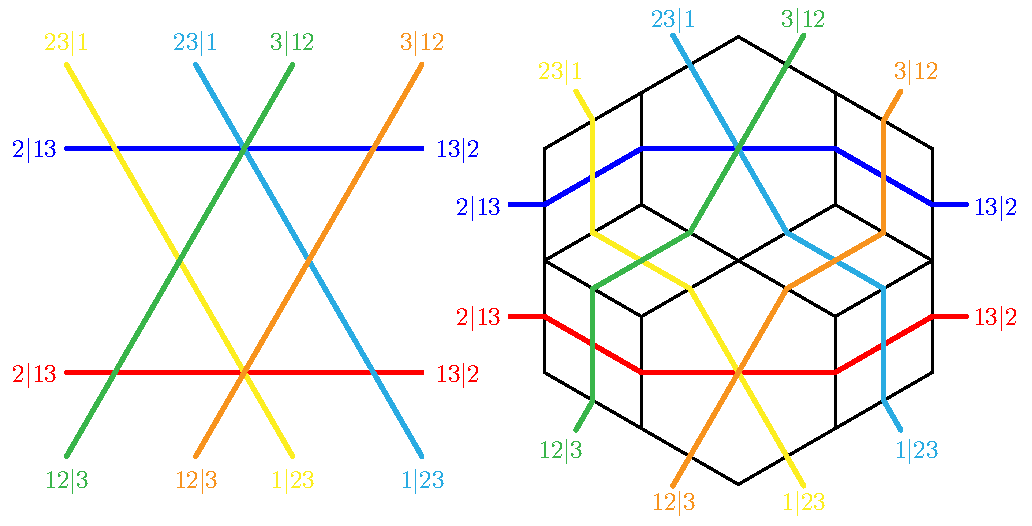
\includegraphics[scale=.9]{diagonalPermutahedron1}
	\caption{The duality between the $(2,3)$-braid arrangement~$\multiBraidArrangement[3][2]$ (left) and the diagonal of the permutahedron~$\Perm[3]$ (right).}
	\label{fig:diagonalPermutahedron1}
\end{figure}

Observe that one can easily compute the full M\"obius polynomials of the $(2,n)$-braid arrangements~$\multiBraidArrangement[n][2]$ from \cref{thm:MobiusPolynomialMultiBraidArrangement}:
\begin{align*}
\mobPol[{\multiBraidArrangement[1][2]}] & = 1 \, , \\
\mobPol[{\multiBraidArrangement[2][2]}] & = x y - 2 x + 2 \, , \\
\mobPol[{\multiBraidArrangement[3][2]}] & = x^2 y^2 - 6 x^2 y + 10 x^2 + 6 x y - 18 x + 8 \, , \\
\mobPol[{\multiBraidArrangement[4][2]}] & = x^3 y^3 - 12 x^3 y^2 + 52 x^3 y - 84 x^3 + 12 x^2 y^2 - 96 x^2 y + 216 x^2 + 44 x y - 182 x + 50 \, , \\
\mobPol[{\multiBraidArrangement[5][2]}] & = x^4 y^4 - 20 x^4 y^3 + 160 x^4 y^2 - 620 x^4 y + 1008 x^4 \\ & \quad+ 20 x^3 y^3 - 300 x^3 y^2 + 1640 x^3 y - 3360 x^3 \\ & \quad+ 140 x^2 y^2 - 1430 x^2 y + 4130 x^2 + 410 x y - 2210 x + 432 \, .
\end{align*}
%which can be encoded in matrices as
%{\small
%\[
%\left(\begin{array}{r}
%1
%\end{array}\right)
%\left(\begin{array}{rr}
%2 & -2 \\
%0 & 1
%\end{array}\right)
%\left(\begin{array}{rrr}
%8 & -18 & 10 \\
%0 & 6 & -6 \\
%0 & 0 & 1
%\end{array}\right)
%\left(\begin{array}{rrrr}
%50 & -182 & 216 & -84 \\
%0 & 44 & -96 & 52 \\
%0 & 0 & 12 & -12 \\
%0 & 0 & 0 & 1
%\end{array}\right)
%\left(\begin{array}{rrrrr}
%432 & -2210 & 4130 & -3360 & 1008 \\
%0 & 410 & -1430 & 1640 & -620 \\
%0 & 0 & 140 & -300 & 160 \\
%0 & 0 & 0 & 20 & -20 \\
%0 & 0 & 0 & 0 & 1
%\end{array}\right)
%%\left(\begin{array}{r}
%%1
%%\end{array}\right)
%%\left(\begin{array}{rr}
%%2 & 0 \\
%%-2 & 1
%%\end{array}\right)
%%\left(\begin{array}{rrr}
%%8 & 0 & 0 \\
%%-18 & 6 & 0 \\
%%10 & -6 & 1
%%\end{array}\right)
%%\left(\begin{array}{rrrr}
%%50 & 0 & 0 & 0 \\
%%-182 & 44 & 0 & 0 \\
%%216 & -96 & 12 & 0 \\
%%-84 & 52 & -12 & 1
%%\end{array}\right)
%%\left(\begin{array}{rrrrr}
%%432 & 0 & 0 & 0 & 0 \\
%%-2210 & 410 & 0 & 0 & 0 \\
%%4130 & -1430 & 140 & 0 & 0 \\
%%-3360 & 1640 & -300 & 20 & 0 \\
%%1008 & -620 & 160 & -20 & 1
%%\end{array}\right)
%%\left(\begin{array}{rrrrrr}
%%4802 & 0 & 0 & 0 & 0 & 0 \\
%%-31922 & 4732 & 0 & 0 & 0 & 0 \\
%%82560 & -23100 & 1830 & 0 & 0 & 0 \\
%%-104400 & 41560 & -6210 & 340 & 0 & 0 \\
%%64800 & -32760 & 6960 & -720 & 30 & 0 \\
%%-15840 & 9568 & -2580 & 380 & -30 & 1
%%\end{array}\right)
%\]
%}

We now focus on the number of vertices, regions, and bounded regions of the $(2,n)$-braid arrangement~$\multiBraidArrangement[n][2]$, to obtain the number of facets, vertices, and internal vertices of the diagonal of the permutahedron~$\Perm$.
The first few values are gathered in \cref{table:enumerationDiagonalPermutahedra1,table:enumerationDiagonalPermutahedra2}.

\begin{table}
	\centerline{\scalebox{1}{
		\begin{tabular}[t]{c|ccccccccccc}
			$n$ & $1$ & $2$ & $3$ & $4$ & $5$ & $6$ & $7$ & $8$ & $9$ & $\dots$ & OEIS \\
			\hline
			facets & $1$ & $2$ & $8$ & $50$ & $432$ & $4802$ & $65536$ & $1062882$ & $20000000$ & $\dots$ & \OEIS{A007334} \\
			vertices & $1$ & $3$ & $17$ & $149$ & $1809$ & $28399$ & $550297$ & $12732873$ & $343231361$ & $\dots$ & \OEIS{A213507} \\
			int. verts. & $1$ & $1$ & $5$ & $43$ & $529$ & $8501$ & $169021$ & $4010455$ & $110676833$ & $\dots$ & \OEIS{A251568}
		\end{tabular}
	}}
	\vspace{.3cm}
	\caption{The numbers of facets, vertices, and internal vertices of the diagonal of the permutahedron~$\Perm$ for~$n \in [9]$.}
	\label{table:enumerationDiagonalPermutahedra1}
\end{table}

\begin{table}
	\centerline{
		\begin{tabular}{c@{\quad}c@{\quad}c@{\quad}c}
			$n = 1$ & $n = 2$ & $n = 3$ & $n = 4$
			\\[.1cm]
			\begin{tabular}[t]{r|c}
				\textbf{dim} & \textbf{0}  \\
				\hline
				\textbf{0} & 1  
			\end{tabular}
			&
			\begin{tabular}[t]{r|cc}
				\textbf{dim} & \textbf{0} & \textbf{1}  \\
				\hline
				\textbf{0} & 3 & 1 \\
				\textbf{1} & 1 &  
			\end{tabular}
			&
			\begin{tabular}[t]{r|ccc}
				\textbf{dim} & \textbf{0} & \textbf{1} & \textbf{2}  \\
				\hline
				\textbf{0} & 17 & 12 & 1 \\
				\textbf{1} & 12 &  6 & \\
				\textbf{2} & 1 &  & 
			\end{tabular}
			&
			\begin{tabular}[t]{r|cccc}
				\textbf{dim} & \textbf{0} & \textbf{1} & \textbf{2} & \textbf{3} \\
				\hline
				\textbf{0} & 149 & 162 & 38 & 1 \\
				\textbf{1} & 162 & 150 & 24 & \\
				\textbf{2} & 38 & 24 & & \\
				\textbf{3} & 1 & & &
			\end{tabular}
		\end{tabular}
	}
	\vspace{.3cm}
	\centerline{
		\begin{tabular}{c@{\quad}c}
			$n = 5$ & $n = 6$
			\\[.1cm]
			\begin{tabular}[t]{r|ccccc}
				\textbf{dim} & \textbf{0} & \textbf{1} & \textbf{2} & \textbf{3} & \textbf{4} \\
				\hline
				\textbf{0} & 1809 & 2660 & 1080 & 110 & 1 \\
				\textbf{1} & 2660 & 3540 & 1200 & 80 & \\
				\textbf{2} & 1080 & 1200 & 270 & & \\
				\textbf{3} & 110 & 80 & && \\
				\textbf{4} & 1 & & & &
			\end{tabular}
			&
			\begin{tabular}[t]{r|cccccc}
				\textbf{dim} & \textbf{0} & \textbf{1} & \textbf{2} & \textbf{3} & \textbf{4} & \textbf{5} \\
				\hline
				\textbf{0} & 28399 & 52635 & 30820 & 6165 & 302 & 1 \\
				\textbf{1} & 52635 & 90870 & 67580 & 7785 & 240 & \\
				\textbf{2} & 30820 & 47580 & 20480 & 2160 & & \\
				\textbf{3} & 6165 & 7785 & 2160 & && \\
				\textbf{4} & 302 & 240 & & &&\\
				\textbf{5} & 1 & & & &&
			\end{tabular}
		\end{tabular}
	}
	\caption{Number of pairs of faces in the cellular image of the diagonal of the permutahedron~$\Perm$ for~$n \in [6]$.}
	\label{table:enumerationDiagonalPermutahedra2}
\end{table}

\begin{corollary}
\label{coro:enumerationDiagonalPermutahedra}
The diagonal of the permutahedron~$\Perm$ has 
\begin{itemize}
\item $2 (n + 1)^{n-2}$ facets,
\item $n \binom{n-1}{k_1} (n-k_1)^{k_1-1} (n-k_2)^{k_2-1}$ facets corresponding to pairs~$(F_1, F_2)$ of faces of the permutahedron~$\Perm$ with~$\dim(F_1) = k_1$ and~$\dim(F_2) = k_2$ (thus~$k_1 + k_2 = n-1$),
\item $\displaystyle n! \, [z^n] \exp \bigg( \sum_{m \ge 1} \frac{C_m \, z^m}{m} \bigg)$ vertices,
\item $\displaystyle (n-1)! \, [z^{n-1}] \exp \bigg( \sum_{m \ge 1} C_m \, z^m \bigg)$ internal vertices,
\end{itemize}
where~$\displaystyle C_m \eqdef \frac{1}{m+1} \binom{2m}{m}$ denotes the $m$\ordinal{} Catalan number.
\end{corollary}

\begin{proof}
Use the duality between the $(2,n)$-braid arrangement~$\multiBraidArrangement[n][2]$ and the diagonal of the permutahedron~$\Perm$ (see \cref{fig:diagonalPermutahedron1}), and specialize \cref{thm:verticesMultiBraidArrangement,thm:regionsMultiBraidArrangement} to~$\ell = 2$.
\end{proof}

\begin{remark}
For completeness, we provide an alternative simpler proof of the first point of \cref{coro:enumerationDiagonalPermutahedra}.
By \cref{prop:flatPosetMultiBraidArrangement}, we just need to count the $(2,n)$-partition trees.
Consider a $(2,n)$-partition tree~$\b{F} \eqdef (F_1,F_2)$ (hence~$\# F_1 + \# F_2 = n + 1$).
Consider the intersection tree~$T$ of~$\b{F}$ with vertices labeled by the parts of~$F_1$ and of~$F_2$ and edges labeled by~$[n]$, root~$T$ at the part of~$F_1$ containing vertex~$1$, forget the vertex labels of~$T$, and send each edge label of~$T$ to the next vertex away from the root, and label the root by~$0$.
See \cref{fig:tree}.
The result is a spanning tree of the complete graph~$K_{n+1}$ on~$\{0, \dots, n\}$ which must contain the edge~$(0,1)$ (because we have chosen the root to be the part of~$F_1$ containing~$1$).
%
\begin{figure}
	\centerline{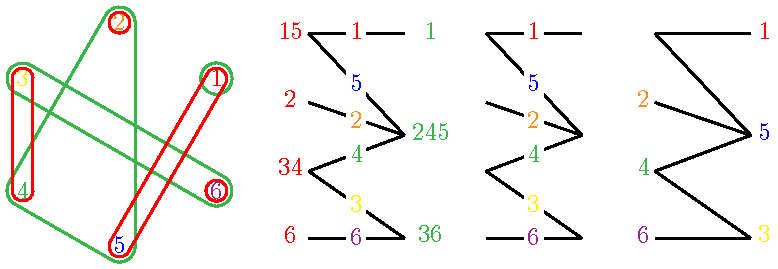
\includegraphics[scale=1]{tree}}
	\caption{The bijection from rooted $(\ell,n)$-partition trees (left) to spanning trees of~$K_{n+1}$ containing the edge~$(0,1)$ (right).}
	\label{fig:tree}
\end{figure}
%
Finally, by double counting the pairs~$(T,e)$ where $T$ is a spanning tree of~$K_{n+1}$ and $e$ is an edge of~$T$, we see that $n$ times the number of spanning trees of~$K_{n+1}$ equals $\binom{n+1}{2}$ times the number of spanning trees of~$K_{n+1}$ containing~$(0,1)$.
Hence, by Cayley's formula for spanning trees of~$K_{n+1}$, we obtain that the number of $(2,n)$-partition trees~is
\[
\frac{2n}{n(n+1)} (n+1)^{n-1} = 2 (n + 1)^{n-2}.
\]
\end{remark}

%%%%%%%%%%%%%%%

\subsection{Cellular diagonals for the permutahedra}
\label{s:diagonals-permutahedra}

Let us first set up some notations that will be of use throughout the paper. 
A set $\sigma_I := \bigcup_{i\in I} \sigma_i$ is a \emph{partition} of $[n]:=\{1,\ldots,n\}$ if $\bigcup_{i\in I} \sigma_i = [n]$ and $\sigma_i \cap \sigma_j = \emptyset$ for $i \neq j$.
The subsets $\sigma_i$ are called \emph{blocks}. 
We denote by $|\sigma|:=|I|$ the size of the partition (its number of blocks).
A partition is \emph{ordered} if the indexing set $I$ is equipped with a total order; in what follows we shall use $I=[k]$ for $k \in \N$. 
We use the shorthand $14|23$ to denote both the unordered  partition $\{\{1,4\},\{2,3\}\}$, and also the ordered partition $(\{1,4\},\{2,3\})$ (when the order is clear from context).

\begin{figure}
	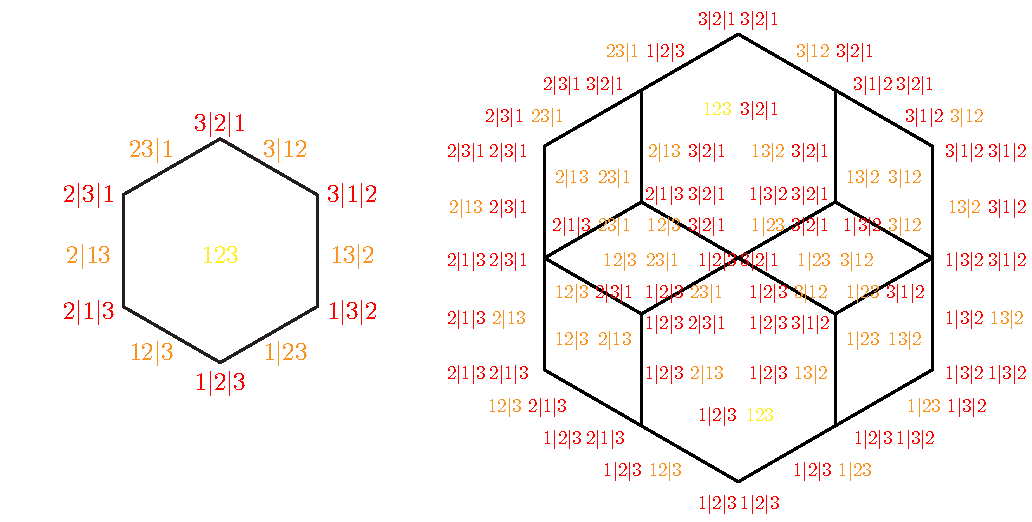
\includegraphics[scale=.9]{diagonalPermutahedron2}
	\caption{Labelings of the faces of the permutahedron~$\Perm[3]$ by ordered partitions of~$[3]$ (left) and of the faces of the LA diagonal  $\LAD$ of the permutahedron~$\Perm[3]$ by pairs of compatible ordered partitions of~$[3]$ (right).}
	\label{fig:diagonalPermutahedron2}
\end{figure}
\vincent{I have included this picture here to be sure that we don't forget it. I should make one for the SU diagonal~$\SUD$ as well.}

Let us recall the universal formula expressing combinatorially the cellular image of the diagonal of a polytope $P$ obtained in \cite[Theorem 1.26]{LA21}.
It is expressed in terms of the \emph{fundamental hyperplane arrangement} of $P$. 

\begin{definition}[Fundamental hyperplane arrangement]
    The \emph{fundamental hyperplane arrangement} $\mathcal{H}_P$ of a polytope $P \subset \R^n$ is the set of hyperplanes whose normal vectors are a choice of directions of the edges of $P\cap \rho_z P$, for any $z \in P$. 
\end{definition}

\begin{example}
    Let $U(n):=\{ (I,J) \ | \ I,J \subset [n], |I|=|J|>0, I \cap J = \emptyset\}$.
    The fundamental hyperplane arrangement of the $(n-1)$-permutahedron is given by the family of hyperplanes \[ \sum_{i \in I} x_i = \sum_{j \in J} x_j \ ,  \ (I,J) \in U(n) \ . \] 
\end{example}

\Guillaume{Mentionner le travail en cours de Lionel Pournin?}

\begin{theorem}[Universal formula]
    \label{thm:universal-formula}
    Let $(P,\vec v)$ be a positively oriented polytope in $\R^n$. 
For each $H\in\mathcal{H}_P$, we choose a normal vector $\vec d_H$ such that $\langle \vec d_H, \vec v \rangle >0$. 
We have 
\begin{eqnarray}
(F,G) \in \Ima \triangle_{(P,\vec v)} 
&\iff& \forall H \in \mathcal{H}_P(F,G), \ \exists i , \ \langle \vec F_i, \vec d_H \rangle < 0  \text{ or } \exists j , \ \langle \vec G_j, \vec d_H \rangle > 0  \\ 
&\iff& \forall H \in \mathcal{H}_P , \ \exists i , \ \langle \vec F_i, \vec d_H \rangle < 0  \text{ or } \exists j , \ \langle \vec G_j, \vec d_H \rangle > 0 \ . 
\end{eqnarray} 
\end{theorem}

Here, the $\vec F_i$ and $\vec G_j$ are vectors spanning the normal cones of the respective faces, and $\mathcal{H}_P(F,G)$ is a subset of hyperplanes which are specifically associated to the pair $(F,G)$.
Applying this Theorem to $P$ the permutahedron, we obtain the following. 

\begin{corollary}
    Any choice of diagonal of the $(n-1)$-permutahedron is given combinatorially by a choice of inequalities \[ \sum_{i \in I} x_i > \sum_{j \in J} x_j \text{ or } \sum_{i \in I} x_i < \sum_{j \in J} x_j \]
    for all $(I,J) \in U(n)$. 
\end{corollary}

\begin{proof}
    A choice of diagonal is given by a choice of vector in a chamber of $\mathcal{H}_P$, two vectors living in the same chamber inducing the same diagonal \cite[Proposition 1.23]{LA21}.
\end{proof}

\vincent{Here, we need to treat all diagonals. Each choice of region in the fundamental hyperplane arrangement gives an orientation of both partitions of a partition forest. We need to explicitly describe this orientation.}

Let us now recall the specific choice of chambers from \cite[Theorem 3.16]{LA21}.

\begin{definition}[$\LA$ diagonal]
    Let $n\geq 1$, and let us write $\LA(n) \coloneqq \{(I,J) \in U(n) \ | \ \min(I\cup J)\in I \}$.
    The \emph{$\LA$ diagonal} $\LAD$ of the $(n-1)$-permutahedron is given by any vector $\vec v \in \R^n$ satisfying  
    \[\sum_{i \in I} v_i > \sum_{j \in J} v_j  \ , \forall (I,J) \in \LA(n) \ . \]
\end{definition}
Applying \cref{thm:universal-formula}, one obtains the following combinatorial description, referred to later as the \emph{$(I,J)$ description}. 
\begin{proposition}
\label{p:minimal}
For a pair $(\sigma,\tau)$ of ordered partitions of $[n]$, we have
\begin{eqnarray*}
    (\sigma,\tau)\in \LAD 
    & \iff & \forall (I,J) \in \LA(\sigma,\tau), \exists k \in [n] , 
    \left| \sigma_{[k]} \cap I \right|
    >
    \left| \sigma_{[k]} \cap J \right| \text{ or } \\
    && \exists l \in [n] , 
    \left| \tau_{[l]} \cap I \right|
    <
    \left| \tau_{[l]} \cap J \right|   \\
    & \iff & \forall (I,J) \in \LA(n), \exists k \in [n] , 
    \left| \sigma_{[k]} \cap I \right|
    >
    \left| \sigma_{[k]} \cap J \right| \text{ or } \\
    && \exists l \in [n] , 
    \left| \tau_{[l]} \cap I \right|
    <
    \left| \tau_{[l]} \cap J \right|  \ . 
\end{eqnarray*}
\end{proposition}
Here, $\LA(\sigma,\tau) \subset \LA(n)$ is a proper subset of $\LA(n)$ which depends on the choice of~$(\sigma,\tau)$, and comes from the geometry of the situation, see \cite[Theorem 1.26]{LA21} for more details.
For our present purposes, it will be enough to restrict our attention to facets of $\LA$, that is pairs $(\sigma,\tau)$ which satisfy $|\sigma| + |\tau|=n+1$.
In this case, the set $\LA(\sigma,\tau)$ has $n-1$ elements, and admits the following description. 

For any subset $\sigma_i \subset [n]$, let $\vec \sigma_i \in \R^n$ denote the boolean vector whose coordinates are given by $1$ in position $j$ if $j \in \sigma_i$ and $0$ otherwise. 
Given a facet $(\sigma,\tau)$ of $\LAD$, one can consider the system of equations $\langle \vec \sigma_i , x \rangle=0$, $\langle \vec \tau_j , x \rangle=0$ given by the blocks of both partitions.
For geometric reasons (see the proof of \cite[Theorem 1.26]{LA21}), the solution of this system is $x=0$. 
Now we will be interested in the solutions of the systems associated to the pairs $(\sigma',\tau)$ and $(\sigma,\tau')$ where~$\sigma'$ (resp.~$\tau'$) has been obtained from $\sigma$ (resp. $\tau$) by merging two adjacent blocks.

\begin{proposition}
\label{p:minimal-IJ-pairs}
    There is a bijection between the set $\LA(\sigma,\tau)$ and the solutions to the systems of equations of the form $(\sigma',\tau)$ and $(\sigma,\tau')$. 
\end{proposition}

\Guillaume{A revoir!! Il faut utiliser le fait que ce sont des facettes!!}

\begin{proof}
    For any $z \in (\mathring \sigma+ \mathring \tau)/2$, the face $\tau \cap \rho_z \sigma$ of $P \cap \rho_z P$ is a vertex of the polytope $P \cap \rho_z P$.
    The faces of the form $\tau \cap \rho_z \sigma'$ and $\tau' \cap \rho_z \sigma$ are the edges of $P\cap \rho_z P$ which are adjacent to the vertex $\tau \cap \rho_z \sigma$. 
    By definition $\LA(\sigma, \tau)$ describes the directions of these edges, and the translation is made as follows: for a given pair $(I,J)$, define the corresponding direction $\vec d$ by its coordinates $d_i:=1$ if $i \in I$, $d_j:=-1$ if $j \in J$, and $d_k:=0$ otherwise.  
    We refer to \cite[Section 1.5]{LA21} for more details.
\end{proof}

We will sometimes refer to the elements of $\LA(\sigma,\tau)$ as the \emph{minimal $(I,J)$-pairs}.

%%%%%%%%%%%%%%%%%%%%%%%%%%%%%%%%%%%%%%

\newpage
\section{Operadic diagonals}

%%%%%%%%%%%%%%%

\subsection{Operadic diagonals for the permutahedra}

We consider the unordered sets $$U(n)  \eqdef  \set{\{I,J\}}{I,J \subset [n], |I|= |J|, I\cap J = \emptyset} \ . $$

\begin{definition}
The $\LA$ and $\SU$ orders on $U=\{U(n)\}$ are defined by 
\begin{itemize} 
    \item $\LA(n) \eqdef \set{(I,J)}{\{I,J\} \in U(n), \ \min(I\cup J) = \min I}$, and by 
    \item $\SU(n) \eqdef \set{(I,J)}{\{I,J\} \in U(n), \ \max(I\cup J) = \max J}$.
\end{itemize}
\end{definition}

As we have seen in the preceding Section, the $\LA$ order defines the diagonal $\LAD$. 
Similarly, we will show in \Guillaume{Corollary X} that the $\SU$ order defines the Saneblidze--Umble diagonal from $\SUD$ \cite{SaneblidzeUmble04}.
Both of these diagonals have opposites $(\LAD)^{\op}$ and $(\SUD)^{\op}$, obtained by permuting the factors in every term; at the level of orderings they are obtained by permuting $I$ and $J$ in the definitions of $\LA(n)$ and $\SU(n)$. 
Geometrically, these opposite versions are given by taking $-\vec v$ instead of $\vec v$ as an orientation vector. 

In general, an \emph{ordering} $O$ of $U$ is a family of sets $\{O(n)\}_{n\geq 1}$ where each $O(n)$ has as elements ordered pairs $(I,J)$ or $(J,I)$, for each $\{I,J\} \in U(n)$.
For an ordered pair $(I,J)$ in $O(n)$, we denote by $\std(I,J)$ the standardisation function, e.g. $\std(\{5,9,10\},\{6,8,12\}) = (\{1,4,5\},\{2,3,6\})$.

\begin{definition}
    \label{def:operadic-ordering}
An ordering $O \eqdef \{O(n)\}_{n \geq 1}$ of $U \eqdef \{U(n)\}_{n\geq 1}$ is \emph{operadic} if for all $(I,J) \in O$, we have that $(I',J') \subsetneq (I,J) \implies \std(I',J') \in O$. 
\end{definition}

We will see \Guillaume{in prop X} that these choice of orderings induce operadic structure on the operahedra, multiplihedra and associahedra.

\begin{lemma} \label{lem:operadic-ordering}
The $\LA$ and $\SU$ orderings are operadic, and are extensions of the following $(I,J)$ pairs,
\begin{itemize}
    \item $\LA :$ for all $k\geq 1$  $(\{1,k+2,k+3,\dots,2k-1,2k\}, \{2,3,\dots,k+1\})$, and 
    \item $\SU :$ for all $k\geq 1$  $(\{k,k+1,\dots,2k-1\},\{1,2,3,\dots,k-1,2k\})$. 
\end{itemize}
The dual orders $\LA^{op}$ and $\SU^{op}$ are also operadic, and extensions of the opposite pairs.
\end{lemma}

\begin{proof}
We present the proof for the $\LA$ ordering, the proofs for the $\SU$ and opposite orders are similar.
First, observe that if an ordered pair $(I,J)$ can be written as $(I_a \sqcup I_b, J_a \sqcup J_b)$ with $(I_a,J_a)$ and $(I_b,J_b)$ in $\LA(|I|)$, then $(I,J)$ is itself in $\LA$.
Second, it is apparent that $(I_k,J_k) \eqdef (\{1,k+2,k+3,\dots,2k-1,2k\}, \{2,3,\dots,k+1\})$ is not a union of other $\LA$ pairs as $1$ is the only element of $I_k$ which is smaller than other elements of $J_k$.
As such, if we try to decompose $(I_k,J_k)$ as a non-trivial union, there is always one pair $(I,J)$ in this union for which $1 \notin I$, so we have $\min ( I \cup J) = \min J$, which implies that $(I,J) \notin \LA$.
Third, we show that any pair $(I,J)$ in $\LA$ which is not of the form $(I_k,J_k)$ can be decomposed as a union of such pairs. 
In combination with the two previous observations, this will prove the Lemma. 

Let $(I,J)$ be in $\LA(k)$ and suppose that $(I,J) \neq (I_k,J_k)$, then there exists $i_2 \in I\ssm \min I$ such that $i_2 < \max J$.
This means that $(I,J)$ can be decomposed as a union: if we write it as $(\{i_1,\dots,i_k\},\{j_1,\dots,j_k\})$, where each set ordered smallest to largest, then we must have $1=i_1<i_2<j_k$, in which case $(\{i_2\},\{j_k\})$ and $(\{i_1,i_3,\dots,i_k\},\{j_1,\dots,j_{k-1}\})$ are both smaller $\LA$ pairs.
Then it must be the case that $\std((\{i_2\},\{j_k\})) = (\{1\},\{2\})$, and $\std((\{i_1,i_3,\dots,i_k\},\{j_1,\dots,j_{k-1}\}))$ is either $(I_{k-1},J_{k-1})$, or we can repeat this decomposition.
This process must eventually terminate with the right-hand side reducing to $(I_l,J_l)$ for some $1 \leq l \leq k-1$.
In other words, any $(I,J) = (\{i_1,\dots,i_k\}, \{j_1,\dots,j_k\})$ decomposes as
\begin{align*}
	(I,J) = (\{i_2\},\{j_k\}) \sqcup (\{i_3\},\{j_{k-1}\}) \sqcup \dots \sqcup (\{i_{l+1} \},\{j_{k-l-1} \}) \sqcup (I',J')
\end{align*}
where $\std((I',J')) = (I_l,J_l)$, and $1\leq l \leq k$.
\end{proof}

We note that the decomposition in \cref{lem:operadic-ordering} is one of potentially many different decompositions of the pair $(I,J)$. 
However, by definition of the $\LA$ order, for any decomposition $(I,J) = (\sqcup_{a\in A} I_a, \sqcup_{a \in A} J_a)$, we have that $\forall a \in A, \std(I_a, J_a) \in \LA$.
As such all decompositions of a pair $(I,J)$ order it the same way.

\begin{proposition}
    \label{prop:operadic-ordering}
The only operadic orderings of $U=\{U(n)\}_{n\geq 1}$ are the $\LA,\SU,\LA^{\op}$ and $\SU^{\op}$ orderings.
\end{proposition}

\begin{proof}
We first observe that there are precisely four ways to order the $U(n)$ pairs of size $k\leq 2$ such that the coherent extension of these orders do not collide.
These are,
\begin{itemize} 
    \item $(\{1\},\{2\})$ and $(\{1,4\},\{2,3\})$ which corresponds to $\LA$ i.e. $\min(I\cup J) = \min I$;
    \item $(\{1\},\{2\})$ and $(\{2,3\},\{1,4\})$ which corresponds to $\SU$ i.e. $\max(I\cup J) = \max J$;
    \item $(\{2\},\{1\})$ and $(\{2,3\},\{1,4\})$ which corresponds to $\LA^{\op}$ i.e. $\min(I\cup J) = \min J$;
    \item $(\{2\},\{1\})$ and $(\{1,4\},\{2,3\})$ which corresponds to $\SU^{\op}$ i.e. $\max(I\cup J) = \max I$.
\end{itemize}
More specifically, we must first order the sole reduced pair $\{\{1\},\{2\}\}$ of $U(1)$.
Then, the sole reduced pair of $U(2)$ which must be ordered is $\{\{1,4\},\{2,3\} \}$.
There are clearly four ways to order these two pairs, and we can identify these $(I,J)$ pairs as cases of \cref{lem:operadic-ordering}.

We now show that once we have committed to one of these four orders we must follow through with it.
We will show this through induction for the $LA$ order, the $\SU$ and opposite orders proceeds similarly.
Let $l\geq 2$ and suppose that for all $k\leq l$, we have ordered $I_k=\{1,k+2,k+3,\dots,2k-1,2k\} < J_k=\{2,3,\dots,k+1\}$.
Then from \cref{lem:operadic-ordering} we know that the only $\{I,J\}$ pair of order $l+1$ that will not decompose (and hence be specified by the already chosen conditions) is $\{I_{l+1},J_{l+1}\}$.
As such, the only way we can vary from $\LA$ is to order this element in the opposite direction i.e. choose $(J_{l+1},I_{l+1})$.
However, this choice leads to contradictions in the ordering of the $\{I,J\}$ pairs of order $|I|=|J|=l+2$.
The following is a generalisation of \cref{ex:Non-coherent order contradiction}.
For $m = l+2$, the pair $\{I_m,J_m\}$ can be oriented in both directions.
On the one side, we can write $\{I_m,J_m\} = \{I_a \cup I_b, J_a \cup J_b\}$ with $I_a \eqdef  \{1,m+3,\dots,2m\} > J_a \eqdef  \{4,5,\dots,m+2\}$  and $I_b \eqdef \{3\} > J_b \eqdef  \{2\}$, which imply that $I_m > J_m$ by the first remark in the proof of \cref{lem:operadic-ordering}. 
This decomposition makes use of the (reversed) order $J_{l+1} > I_{l+1}$ and the (non-reversed) order $I_1 < J_1$.
On the other side, we can write $\{I_m,J_m\} = \{I_c \cup I_d, J_c \cup J_d\}$, where $I_c \eqdef  \{1,m+3,\dots,  2m-1\} < J_c \eqdef  \{2,5,\dots,m+1\}$ and $I_d \eqdef \{3, 2m\} < J_d \eqdef  \{4, m+2\}$, which imply that $I_m < J_m$ via the (non-reversed) orders $I_l < J_l$ and $I_2 < J_2$, a contradiction.
\end{proof}

\begin{example} 
\label{ex:Non-coherent order contradiction}
Suppose that the $\LA$ order holds for pairs of order $1$ and $2$, but is reversed for pairs of order $3$, i.e. we have 
\begin{align*}
    \{1\}<\{2\},\quad \{1,4\}< \{2,3\}, \text{ and } \{1, 5, 6 \} > \{2, 3, 4\} \ .
\end{align*}
Then $\{I,J\}=\{\{1, 3, 7, 8\}, \{2, 4, 5, 6\}\}$ admits two different orientations.
In particular, 
\begin{align*}
    \{1, 7, 8\} > \{ 4, 5, 6 \} \text{ and } \{3\} > \{2\} &\implies \{1, 3, 7, 8\} >\{2, 4, 5, 6\} \ \text{and} \\
    \{1, 7\}< \{2, 5\} \text{ and } \{3, 8\}< \{4, 6\} &\implies \{1, 3, 7, 8\} <\{2, 4, 5, 6\} \ .
\end{align*}
\end{example}

Now recall that each face $A_1 | \ldots | A_k$ of the permutahedron $P_{|A_1|+\cdots + |A_k|-1}$ is isomorphic to the product $P_{|A_1|-1} \times \cdots \times P_{|A_k|-1}$ of lower dimensional permutahedra, via the isomorphism
\begin{equation*}
    \begin{matrix}
        \Theta & : & \R^{|A_1|} \times \cdots \times \R^{|A_k|} & \overset{\cong}{\longrightarrow} & \R^{|A_1|+\cdots+|A_k|} \\
         & & (x_1,\ldots,x_{|A_1|}) \times \cdots \times (x_{|A_1|+\cdots +|A_{k-1}|+1}, \ldots, x_{|A_1|+\cdots +|A_k|})  & \mapsto & (x_{\sigma^{-1}(1)},\ldots,x_{\sigma^{-1}(|A_1|+\cdots +|A_k|)})
    \end{matrix}
\end{equation*}
where $\sigma$ is the $(|A_1|,\ldots,|A_k|)$-shuffle sending the increasingly ordered elements of~$A_1 \cup \ldots \cup A_k$ to the block by block increasingly ordered elements of $A_1 | \ldots | A_k$.
Note that this map is a particular instance of the eponym map introduced in Point (5) of \cite[Prop. 2.3]{LA21}.

\begin{remark}
    This fact underlies a \emph{permutadic} structure \cite{LodayRonco11,MARKL2020105277}.
\end{remark}

A \emph{diagonal of the permutahedra} $\triangle:=\{\triangle_n\}$ is a family of diagonals $\triangle_n : P_n \to P_n \times P_n$, for each $n$-permutahedron $P_n$, $ n \geq 1$. 

\begin{definition}
    A diagonal of the permutahedra $\triangle$ is \emph{operadic} if for every face $A_1 | \ldots | A_k$ of the permutahedron $P_{|A_1|+\cdots + |A_k|-1}$, the map $\Theta$ induces a topological cellular isomorphism \[  \triangle(A_1) \times \ldots \times \triangle(A_k) \cong \triangle(A_1 | \ldots | A_k) \ . \]
\end{definition}
In other words, we require that the diagonal $\triangle$ commutes with the map $\Theta$, see \cite[Section 4.2]{LA21}.
At the algebraic level, this property is called ``comultiplicativity" in \cite{SaneblidzeUmble04}.
\Guillaume{Our choice of terminology comes from the results in Section X}
Note that in particular such an isomorphism respects the poset structures. 

\begin{theorem}
\label{prop:unique-operad}
There are exactly four operadic diagonals on the permutahedra. 
\end{theorem}

\begin{proof}
    First, by \cite[Theorem 3.9]{LA21} any diagonal in the sense of \cref{def:diagonal} is given by a choice of ordering of $U$.
    Second, every operadic diagonal satisfies \cite[Proposition 4.14]{LA21}, which amounts precisely to an operadic ordering of $U$ in the sense of \cref{def:operadic-ordering}.
    We conclude with \cref{prop:operadic-ordering}.
\end{proof}

The orientation vectors $\vec v=(v_1,\ldots,v_{n}) \in \R^n$ inducing each of these four diagonals are given by the conditions \[ \sum_{i \in I} v_i > \sum_{j \in J} v_j \ , \ \forall (I,J) \in O(n) \ , \]
where $O(n)$ stands for either $\LA(n), \LA(n)^\op, \SU(n)$ or $\SU(n)^\op$.

\begin{remark}
    This answers by the negative a conjecture regarding unicity of diagonals on the permutahedra, raised at the beginning of \cite[Section 3]{SaneblidzeUmble04}, and could be seen as a ``corrected" version of it. \Guillaume{See the next section where we prove that SU diagonal is SU diagonal}
\end{remark}

%%%%%%%%%%%%%%%

\subsection{Isomorphisms between permutahedra's operadic diagonals}

Let $P$ be a centrally symmetric polytope, and let $s : P \to P$ be its involution, given by taking a point $p \in P$ to its reflection $s(p)$ with respect to the center of symmetry of $P$. 
Note that this map is cellular, and induces an involution on the face lattice of $P$. 
For $P$ the permutahedron, this face poset involution is given by the assignment $A_1 | \cdots | A_k \mapsto A_k | \cdots | A_1$. 

The permutahedron possesses another symmetry: the cellular involution $r : P \to P$ which sends a point $p \in P$ to its reflection with respect to the hyperplane of equation \[ \sum_{i=1}^{\lfloor n/2 \rfloor}x_i = \sum_{i=1}^{\lfloor n/2 \rfloor}x_{n-i+1} \ . \]
This involution also respects the face poset structure. 
In terms of ordered partitions, it replaces each block $A_j$ in $A_1 | \cdots | A_k$ by the block $r(A_j):=\{n-i+1 \ | \ i \in A_j\}$.

As we have already remarked \Guillaume{in Rem X}, the polytope of diagonals of $P$ is always centrally symmetric, and the involution $t : P \times P \to P \times P$ sending $(x,y)$ to~$(y,x)$ takes a cellular diagonal to another cellular diagonal.
In the case of the permutahedron it sends $\LAD$ to $(\LAD)^\op$ and $\SUD$ to $(\SUD)^\op$.

\begin{theorem}
    \label{thm:bijection-operadic-diagonals}
    For $P$ the permutahedron, the involutions $t$ and $rs \times rs$ are cellular isomorphisms between the four operadic diagonals, through the following commutative diagram: 
    \begin{center}
        \begin{tikzcd}
        \LAD \arrow[r,"t"] \arrow[d,"rs \times rs"]&
        (\LAD)^{\op}\arrow[d,"rs \times rs"]\\
        \SUD \arrow[r,"t"] &
        (\SUD)^\op
        \end{tikzcd}
        \end{center}
    Moreover, they induce poset isomorphisms at the level of the face lattices. 
\end{theorem}

\begin{proof}
    The result for the transpositions $t$ and the commutativity of the diagram are straighforward, so we prove that $rs\times rs$ is a cellular isomorphism respecting the poset structure. 
    First, we observe that the assignment $(I,J) \mapsto (r(J),r(I))$ defines a bijection between $\LA(n)$ and $\SU(n)$. 
    Indeed, we have $r(\min(I\cup J))=\max(I\cup J)$; since $I \cap J = \emptyset$, $r$ is well-defined, and it is a bijection with inverse $r$ itself.  
    Denoting by $N^c$ the complement of a subset $N \subset [n]$, we have that $|N \cap I| > |N\cap J| \iff |N^c \cap I|< |N^c \cap J|$.
    Combining this with the fact that $|N \cap I| > |N\cap J| \iff |r(N) \cap r(I)| > |r(N) \cap r(J)|$, we obtain that 
    \begin{eqnarray*}
        |N \cap I| > |N\cap J| \iff |r(N)^c \cap r(I)| < |r(N)^c \cap r(J)| \ .
    \end{eqnarray*}
    Similarly, we have $|N' \cap I| < |N'\cap J| \iff |r(N')^c \cap r(I)| > |r(N')^c \cap r(J)|$, so that $(\sigma,\tau) \in \LAD$ if and only if $(rs(\sigma),rs(\tau)) \in \SUD$. 
    Finally, since both $t,r$ and $s$ preserve the poset structures, so does their composition, which finishes the proof.
\end{proof}

\begin{remark} \label{rem:Alternate Isomorphism}
There is a second, distinct isomorphism given by $t(r\times r)$.
This follows as $s\times s:\LAD \to (\LAD)^{op}$ is an isomorphism (and also for  $s\times s:\SUD \to (\SUD)^{op}$ ), as such the composite 

\begin{center}
\begin{tikzcd}
t(r\times r):\LAD \arrow[r,"s\times s"] &
(\LAD)^{\op}\arrow[r,"rs \times rs"] &
(\SUD)^\op \arrow[r,"t"] & \SUD
\end{tikzcd}
\end{center}
is also an isomorphism.
We will show this second isomorphism has the conceptual benefit of sending left shift operators to left shift operators (and right to right) in \cref{prop:trr is an isomorphism of shifts}.

\end{remark}

%%%%%%%%%%%%%%%

\subsection{Facets of operadic diagonals}

We have seen in \cref{subsec:multiBraidArrangement} that facets of any diagonal of the permutahedron are in bijection with $(2,n)$-trees, that is, a pair of partitions whose intersection graph is a tree.
These are precisely the \emph{essential complementary partitions} studied in \cite{chen1969computer,chen1971tables,kajitani1982number}. 
Here, we describe a specific planar embedding of the $(2,n)$-trees for each operadic diagonal. 
\Guillaume{Simplify and unify exposition with Section 1}

\begin{definition}
A set of \emph{distinct representatives} of an (unordered) partition $\sigma_I$ is a set $M\subset [n]$ such that $\forall i \in I,|\sigma_i \cap M| = 1$.
\end{definition}

\begin{definition}
A pair of partitions $(\sigma_L,\tau_R)$ is 
\begin{enumerate} 
    \item \emph{complementary} if there exists $M\subset [n]$ and $m \in M$ such that $M$ and $([n]\ssm M) \cup \{m\}$ are distinct representatives of $\sigma_L$ and $\tau_R$, respectively,
    \item it is furthermore \emph{essential} if there does not exist proper subsets $ L'\subset L$, $R'\subset R$ and $N \subset [n]$ such that $(\sigma_{L'},\tau_{R'})$ is a complementary partition of $N$.
\end{enumerate}
\end{definition}

An equivalent definition is the following. 

\begin{definition}
A pair of partitions $(\sigma_L,\tau_R)$ is said to be 
\begin{enumerate}
	\item \emph{complementary}, if $\forall l\in L, r\in R$ we have that $|\sigma_l \cap \tau_r| \leq 1$,
	\item \emph{essential}, if there are no proper subsets of $L'\subset L,R'\subset R$ such that $\cup_{l \in L'} \sigma_l = \cup_{r \in R'} \tau_r$.
\end{enumerate}	
\end{definition}

In cases where there is no ambiguity, we will drop the subscripts $L,R$.
We shall denote the set of all essential complementary pairs of partitions of $[n]$ by $\EC$.
Let us emphasise that the pairs of partitions of $\EC$ are \emph{unordered}.

\begin{example}
For $n=2$, the two essential complementary partitions are $1|2 \times 12$ and $12 \times 1|2$. For $n=3$, the eight essential complementary partitions are
\begin{align*}
	1|2|3 \times 123,\quad 
	123 \times 1|2|3,\quad 
	1|23 \times 13|2,\quad 
	13|2 \times 1|23\\
	1|23 \times 12|3,\quad 
	12|3 \times 1|23,\quad 
	13|2 \times 12|3,\quad 
	12|3 \times 13|2
\end{align*}
For a larger example, see \cref{ex:ECbijection}. 
\end{example}

%A \emph{tree} is a simply connected graph with no cycles. 
%A \emph{bipartite graph} is a graph whose vertices are partitioned into two sets such that vertices in one set are only adjacent to vertices in the other.
%We say a bipartite graph is \emph{ordered} if one of the sets is considered smaller than the other and we denote the partition $(V_L,V_R)$. 
%We say a graph with $n$ edges is \emph{edge labelled} if there exists a bijection between the edges and $\{1,\dots,n\}$.

As we have seen in \cref{subsec:multiBraidArrangement}, essential complementary partitions are in bijection with $(2,n)$-trees.
Given an essential complementary pair $(\sigma,\tau)$, the corresponding $(2,n)$-tree has the blocks of each partition as its vertices, and two such vertices are connected by an edge if the two blocks share a common element, which labels the edge, see \cref{ex:ECbijection}.


\begin{theorem}
\label{thm:facets}
The facets of any operadic diagonal $\OP$ are in bijection with essential complementary partitions, through the inverse functions $u:\OP \to \EC$ and $o:\EC\to \OP$, where
\begin{enumerate}
    \item the function $u$ forgets the order of the ordered partition pair,
    \item the function $o$ uniquely orders an essential complementary partition pair via the minimal $(I,J)$-pairs defining the diagonal. 
\end{enumerate}
In particular, this defines a particular planar embedding of each $(2,n)$-tree, as illustrated in \cref{ex:ECbijection}.
\end{theorem}

We shall prove this theorem by establishing the necessary total order, showing that the functions are well defined, and then showing that they are injective.
We will work with the $\LAD$ diagonal, but the proofs can be straightforwardly modified to accommodate any of the other three operadic diagonals. 

\begin{lemma} 
\label{l:u-well-defined}
The function $u:\OP \to \EC$ that forgets the order in a pair of partitions is well defined.
\end{lemma}
\begin{proof}
Let $(\sigma,\tau)$ be a pair of ordered partitions forming a facet of $\LAD$. 
Their intersection graph has $n+1$ vertices and $n$ edges, and as no vertices can be isolated it must be a tree. 
%It is straightforward to verify that it must be a labeled bipartite tree, but here is how we may explicitly produce the necessary distinct representatives using an algorithm of \cite[Theorem 2]{kajitani1982number}.
%Let $G'$ be a copy of $G(u(P))$. 
%While there is a vertex of degree $1$ in $G'$ delete it and add the sole edge of that vertex as a distinct representative of the corresponding partition of that vertex. 
%As $G'$ is a tree this process can continue until there is a single edge connecting two vertices of degree $1$. 
%This edge specifies the element $p$ of the distinct representatives.
\end{proof}

\begin{construction} 
\label{const:total}
For $(\sigma,\tau) = (\bigcup_{l\in L}\sigma_l,\bigcup_{r\in R} \tau_r)$ an essential complementary pair, we construct total orders on the blocks of $\sigma$ and $\tau$ in three steps:
\begin{enumerate}
    \item For any two blocks $\sigma_k,\sigma_l$ in $\sigma$ or $\tau$, there is a unique minimal path $\gamma$ of even cardinality  connecting them.
    We partition $\gamma=I\cup J$ where $\min(I\cup J) \in I$ and the path alternates between elements of $I$ and $J$;
    \item Direct each path $\gamma$ so that all the edges of $I$ (resp. $J$) go from left to right (resp. right to left);
    \item We say $\sigma_k< \sigma_l$ if the path joining them is directed from $\sigma_k$ to $\sigma_l$.
\end{enumerate}
\end{construction}

\begin{proof}
We first show our binary relation is well defined before verifying that it defines a total order on the vertices of the $(2,n)$-tree.
In a bipartite tree, every vertex is connected, and every path connecting two vertices on the same side must be of even length. 
As $I$ and $J$ partition the path in an alternating fashion, i.e. $\gamma=(i_1,j_1,i_2,j_2,\dots)$, we can orient it by forcing each edge of $I$ (resp. $J$) to point to the right (resp. left). 
This order is clearly total, reflexive (by convention) and anti-symmetric, what remains to be checked is its transitivity. 

Let $\gamma$ denote the unique maximal path between two vertices $a$ and $b$ on the left of the tree, that is two blocks of $\sigma$. 
Let $I_{ab}$ denote the set of left-to-right edges in this path, and let $J_{ab}$ denote its complement. 
Then, we have 
\begin{equation}
    \label{eq:order}
    a < b \iff \min(I_{ab}\cup J_{ab})=\min(I_{ab}) \ . 
\end{equation}
Suppose now that $a < b$ and $b < c$.
Since $\gamma_{ac}= (\gamma_{ab} \cup \gamma_{bc}) \ssm (\gamma_{ab} \cap \gamma_{bc})$, we have $$ I_{ac}=(I_{ab}\cup I_{bc}) \ssm (J_{ab} \cup J_{bc}) \text{ and } J_{ac}=(J_{ab}\cup J_{bc}) \ssm (I_{ab} \cup I_{bc}) \ , $$ and from the condition (\ref{eq:order}) above, it is clear that $\min(I_{ac}\cup J_{ac})=\min(I_{ac})$, which completes the proof of the transitivity for the total order on $\sigma$. 
The proof for $\tau$ is similar. 
\end{proof}

\begin{example}
\label{ex:ECbijection}
We now illustrate the ordering (right) of the pair of essential complementary partitions $\{15,234,6,7\} \times \{13,2,46,57\}$ (left).
\begin{center}
\begin{tikzpicture}[scale=.7]  
\node (1) at (-1.5, -1) {$15$};
\node (2) at (-1.5, -2) {$234$};
\node (3) at (-1.5, -3) {$6$};
\node (4) at (-1.5, -4) {$7$};
%
\node (5) at (1.5, -1) {$13$};
\node (6) at (1.5, -2) {$2$};
\node (7) at (1.5, -3) {$46$};
\node (8) at (1.5, -4) {$57$};
%
\draw[thick] (1) to [in=180, out=0, looseness=0] (5); 
\draw[thick] (1) to [in=180, out=0, looseness=0] (8);
\draw[thick] (2) to [in=180, out=0, looseness=0] (5); 
\draw[thick] (2) to [in=180, out=0, looseness=0] (6); 
\draw[thick] (2) to [in=180, out=0, looseness=0] (7); 
\draw[thick] (3) to [in=180, out=0, looseness=0] (7);
\draw[thick] (4) to [in=180, out=0, looseness=0] (8);
%
\end{tikzpicture}
$\quad$
\begin{tikzpicture}[scale=.7]  
\node (1) at (-1.5, -1) {$15$};
\node (2) at (-1.5, -2) {$7$};
\node (3) at (-1.5, -3) {$234$};
\node (4) at (-1.5, -4) {$6$};
%
\node (5) at (1.5, -1) {$57$};
\node (6) at (1.5, -2) {$46$};
\node (7) at (1.5, -3) {$13$};
\node (8) at (1.5, -4) {$2$};
%
\draw[thick] (1) to [in=180, out=0, looseness=0] (5); 
\draw[thick] (1) to [in=180, out=0, looseness=0] (7);
\draw[thick] (2) to [in=180, out=0, looseness=0] (5); 
\draw[thick] (3) to [in=180, out=0, looseness=0] (6); 
\draw[thick] (3) to [in=180, out=0, looseness=0] (7); 
\draw[thick] (3) to [in=180, out=0, looseness=0] (8); 
\draw[thick] (4) to [in=180, out=0, looseness=0] (6);
%
\end{tikzpicture}
\end{center}
Here are two examples of paths providing order information, with $(I,J)=(\{1,7\},\{3,5\})$ and $(I,J)=(\{1,4\},\{3,5\})$
\begin{align*}
	7 <_L 234 \text{ as } 7 \xrightarrow{7} 57 \xrightarrow{5} 15 \xrightarrow{1=\min(I\cup J)} 13 \xrightarrow{3} 234 \ , \\
	57 <_R 46 \text{ as } 57 \xrightarrow{5} 15 \xrightarrow{1=\min(I\cup J)} 13 \xrightarrow{3} 234 \xrightarrow{4} 46 \ .
\end{align*}
\end{example}

This order far from being arbitrary provides the unique way to order an essential complementary partition pair into an ordered partition pair of $\LAD$, as we shall demonstrate next.
First, we need a geometrical result. 

\begin{proposition}
    \label{prop:geometrical-IJ}
    The paths between adjacent vertices of $\sigma$ or $\tau$ are in bijection with the minimal $(I,J)$-pairs (see \cref{s:diagonals-permutahedra}).
\end{proposition}

\begin{proof}
    By \cref{p:minimal-IJ-pairs}, it suffices to show that the paths between adjacent vertices of $\sigma$ are in bijection with the solutions of the system of equations of the form $(\rho^1,\sigma^2)$. 
    To ease notation, let us write $\rho$ for $\rho^1$ and $\sigma$ for $\sigma^1$. 
    Suppose that $\rho$ is obtained from $\sigma$ by merging the two blocks $\sigma_a$ and $\sigma_b$. 
    The two equations $\langle \vec \sigma_a, x \rangle =0$ and $\langle \vec \sigma_b, x \rangle =0$ now become $\langle \vec \sigma_a + \vec \sigma_b, x \rangle =0$; nothing else changes in the system. 
    Since the solution to the system $(\sigma^1,\sigma^2)$ was $x=0$, now the solution is of dimension $1$, and it is given precisely by the path between $a$ and $b$.
    Such a path is given by an alternating sequence of vertices and edges $\sigma_1 \eqdef \sigma_a, e_1, \sigma_2, e_2, \ldots, e_{k-1}, \sigma_k \eqdef \sigma_b$. 
    Every edge $e_i \in \{1,\ldots, n\}$ is by definition the intersection $\sigma_{i} \cap \sigma_{i+1}$; thus it is the only common non-zero coordinate between $\vec \sigma_{i}$ and $\vec \sigma_{i+1}$.
    Thus, the path encodes the series of equations $x_{e_1}+x_{e_{k-1}}=0$, $x_{e_1}+x_{e_2}=0$, $x_{e_2}+x_{e_3}=0$, $\ldots$, $x_{e_{k-2}}+x_{e_{k-1}}=0$. 
    Thus, $x_{e_1}=1$, $x_{e_2}=-1$, $x_{e_3}=1$, $\ldots$, $x_{e_{k-2}}=1$, $x_{e_{k-1}}=-1$ is a basis of one-dimensional space of solutions, and it gives the corresponding minimal $(I,J)$-pair. 
\end{proof}

\begin{lemma} 
\label{l:o-well-defined}
The function $o:\EC \to \LAD$ which orders an essential complementary pair is well defined.
\end{lemma}

\begin{proof}
Consider the ordering $o(\sigma,\tau)$ of the pair $(\sigma,\tau)$ given by \cref{const:total}. 
We first show that every $(I,J)$-condition, for $(I,J) \in \LA(n)$, which corresponds to a path between vertices is satisfied. 
In particular, this statement will be true for paths between adjacent vertices, which are exactly the minimal $(I,J)$-pairs according to \cref{prop:geometrical-IJ}.
This will in turn allow us to conclude since testing the minimal $(I,J)$-pairs is equivalent to testing all $(I,J)$-pairs as stated in \cref{p:minimal}. 
Suppose that $I,J$ corresponds to a path between two vertices on the left, i.e.
\begin{align*}
    \sigma_l = \sigma_{l_1} \xrightarrow{i_1} \tau_{r_1}\xrightarrow{j_1} \sigma_{l_2} \xrightarrow{i_2}\dots \xrightarrow{i_{k}} \tau_{r_{k-1}} \xrightarrow{j_k} \sigma_{l_k}= \sigma_{l'}
\end{align*}
By construction we have that $(I = \{i_1,\dots,i_k\},J=\{j_1,\dots,j_k\}) \in \LA(n)$ (note we are ordering $I$ and $J$ by the path, so it is not necessarily the case that $\min I = i_1$). 
Furthermore, each block of $\tau$ either contains a single element of $I$ and a single element of $J$, or it contains no elements of $I$ and no elements of $J$. 
As such, for any ordering of the blocks of $\tau$ we have that
\begin{align*}
    \forall m, \bigg|\bigcup_{1\leq k \leq m} \tau_{k} \cap I \bigg| = \bigg|\bigcup_{1\leq k \leq m} \tau_{k} \cap J \bigg| \ .
\end{align*}
Hence in order for this $\LA(n)$ condition to be satisfied it must be the case that for some ordering of the blocks of $\sigma$ we have
\begin{align*}
    \exists m, \bigg| \bigcup_{1\leq k \leq m} \sigma_k \cap I \bigg| > \bigg|\bigcup_{1\leq k \leq m} \sigma_k \cap J \bigg| \ .
\end{align*}
Every block of $\sigma$ excluding $\sigma_l$ and $\sigma_{l'}$ either contains no elements of both $I$ and $J$, or contains a single element of $I$ and a single element of $J$. 
So the only way for the condition to be satisfied is for $\sigma_l$ to come before $\sigma_{l'}$, which is precisely what is required by the total order.
If the sets $(I,J)$ correspond to a path between two vertices on the right
\begin{align*}
    \tau_r = \tau_{r_1} \xrightarrow{j_1} \sigma_{l_1}\xrightarrow{i_1} \tau_{r_2} \xrightarrow{j_2}\dots \xrightarrow{j_{k}} \sigma_{l_{k-1}} \xrightarrow{1_k} \tau_{r_k}=\tau_{r'} \ ,
\end{align*}
then a similar chain of logic implies we must have an ordering of the blocks of $\tau$ such that
\begin{align*}
    \exists m, \bigg|\bigcup_{1\leq k \leq m}\tau_k \cap I\bigg| < \bigg|\bigcup_{1\leq k \leq m} \tau_k \cap J\bigg| \ , 
\end{align*}
and this can only happen if $\tau_r$ comes before $\tau_{r'}$.
\end{proof}

\begin{remark}
    It would be interesting to know if there is a geometrical interpretation of the paths that are not between adjacent vertices. 
\end{remark}

To complete the proof of \cref{thm:facets}, it remains to show that both $u:\LAD \to \EC$ and $o:\EC\to \LAD$ are injective, with the other function being their inverse.

\begin{proof}[{Proof of \cref{thm:facets}}]
The forgetful function $u$ is clearly the inverse to $o$, as forgetting any assigned order will clearly return the original essential complementary partition pair. 
The ordering function $o$ is the inverse to $u$, as it returns the sole ordering of the blocks which is compatible with the $\LA(n)$ conditions.
\end{proof}

So, we have the follow characterisation of facets of the $\LAD$ and $\SUD$ diagonals (the second one being obtained by changing slightly \cref{const:total} according to the definition of the $\SU$ order).
We omit the adaptation for the two opposite diagonals, which is immediate.

\begin{corollary} 
\label{prop:LAD-ordered-EC}
The facets of the $\LAD$ (resp. $\SUD$) diagonal are ordered essential complementary partitions in which the minimal (resp. maximal) element of each path is traversed from left to right (resp. right to left).
\end{corollary}

We illustrate how the bijection $rs\times rs$ from \cref{thm:bijection-operadic-diagonals} relates the two results.

\begin{example}
\label{ex:theta-path-translation}
We apply the bijection $rs\times rs$ to the element of $\LAD$ from \cref{ex:ECbijection}
\begin{center}
\begin{tikzpicture}[scale=.7]  
\node (1) at (-1.5, -1) {$15$};
\node (2) at (-1.5, -2) {$7$};
\node (3) at (-1.5, -3) {$234$};
\node (4) at (-1.5, -4) {$6$};
%
\node (5) at (1.5, -1) {$57$};
\node (6) at (1.5, -2) {$46$};
\node (7) at (1.5, -3) {$13$};
\node (8) at (1.5, -4) {$2$};
%
\draw[thick] (1) to [in=180, out=0, looseness=0] (5); 
\draw[thick] (1) to [in=180, out=0, looseness=0] (7);
\draw[thick] (2) to [in=180, out=0, looseness=0] (5); 
\draw[thick] (3) to [in=180, out=0, looseness=0] (6); 
\draw[thick] (3) to [in=180, out=0, looseness=0] (7); 
\draw[thick] (3) to [in=180, out=0, looseness=0] (8); 
\draw[thick] (4) to [in=180, out=0, looseness=0] (6);
%
\end{tikzpicture}
\quad
\raisebox{3em}{$\xrightarrow{rs\times rs}$}
\quad
\begin{tikzpicture}[scale=.7]  
\node (1) at (1.5, -4) {$13$};
\node (2) at (1.5, -3) {$24$};
\node (3) at (1.5, -2) {$57$};
\node (4) at (1.5, -1) {$6$};
%
\node (5) at (-1.5, -4) {$37$};
\node (6) at (-1.5, -3) {$1$};
\node (7) at (-1.5, -2) {$456$};
\node (8) at (-1.5, -1) {$2$};
%
\draw[thick] (1) to [out=180, in=0, looseness=0] (5);
\draw[thick] (1) to [out=180, in=0, looseness=0] (6); 
\draw[thick] (2) to [out=180, in=0, looseness=0] (7);
\draw[thick] (2) to [out=180, in=0, looseness=0](8);
\draw[thick] (3) to [out=180, in=0, looseness=0] (5); 
\draw[thick] (3) to [out=180, in=0, looseness=0] (7);
\draw[thick] (4) to [out=180, in=0, looseness=0] (7);
%
\end{tikzpicture} \ .
\end{center}
Observe that the $\LA(7)$ conditions corresponding to paths, such as $( \{1,4\},\{3,5\}) \in \LA(7)$
\begin{align*}
    57 <_R 46 \text{ as } 57 \xrightarrow{5} 15 \xrightarrow{1=\min(I\cup J)} 13 \xrightarrow{3} 234 \xrightarrow{4} 46
\end{align*}
are mapped to $\SU(7)$ conditions corresponding to paths, e.g. the prior $(I,J)$-condition maps to $(r(J),r(I))=( \{3,5 \},\{4,7\}) \in \SU(7)$, and
\begin{align*}
    24 <_R 13 \text{ as } 24 \xrightarrow{4} 456 \xrightarrow{5} 57 \xrightarrow{7=\max(r(J)\cup r(I))} 37 \xrightarrow{3} 13 \ .
\end{align*}
\end{example}
Note that the composite $\LAD \xrightarrow{u} \EC \xrightarrow{o} \SUD$ provides another bijection between facets, however this map is not equal to $rs \times rs$ and is not defined on the other faces.

%%%%%%%%%%%%%%%

\subsection{Vertices of operadic diagonals}

We are now interested in characterizing the pairs of vertices that occur in the diagonal, that is, pairs of permutations $(\sigma_1,\sigma_2) \in \triangle$. 

\begin{theorem} There exists $(I,J) \in D(n)$ such that $\forall k, |\sigma_1^1\cdots\sigma_1^k \cap I| \leq |\sigma_1^1\cdots\sigma_1^k \cap J|$ and $\forall l, |\sigma_1^1\cdots\sigma_1^l \cap I| \geq |\sigma_1^1\cdots\sigma_1^l \cap J|$ (diagonal condition) if and only if $\exists (I',J')=(\{i_1,\ldots,i_m\},\{j_1,\ldots,j_m\}) \in D(m)$, $m\leq n$, such that \[\sigma_1 \cap (I'\cup J')=j_1 i_1 j_2 i_2 \cdots j_n i_n \] and \[ \sigma_2 \cap (I'\cup J') = i_2 j_1 i_3 j_2 \cdots i_n j_{n-1} i_1 j_n \ , \] where $i_1 = \min (I' \cup J')$ (fish condition). 
\end{theorem}

\begin{proof}
\begin{itemize}
\item If a pair of permutations $(\sigma_1, \sigma_2) \in   \mathfrak{S}_N^2$ satisfies the fish condition, then there exist two sets $I$ and $J$ of same cardinality such that $\min(I)<\min(J)$. Denoting $\sigma_1$ and $\sigma_2$ by two words of size $N$ $\sigma_1^1 \ldots \sigma_1^N$ and $\sigma_2^1 \ldots \sigma_2^N$, then the pair $((\sigma_1, \sigma_2), (I,J))$ satisfies that for any $k$ in $\llbracket 1;N\rrbracket$, $|\sigma_1^1 \ldots \sigma_1^k \cap J| \geq |\sigma_1^1 \ldots \sigma_1^k \cap I|$ and $|\sigma_2^1 \ldots \sigma_2^k \cap I| \geq |\sigma_2^1 \ldots \sigma_2^k \cap J|$, hence the diagonal condition.
\item We will now prove the converse. Let us presume that $(\sigma_1, \sigma_2)$ is a pair of permutations satisfying the diagonal condition for a pair of sets $(I,J) \in D(n)$, minimal for the inclusion of sets.
\begin{description}
\item[Case $n=1$] 
\end{description}
If $|I|=|J|=1$, then it follows directly from the diagonal condition above that ${\sigma_1}_{| I \cup J}=j_1 i_1$ and ${\sigma_1}_{|I \cup J}=i_1 j_1$, hence the fish condition is satisfied.
\begin{description}
\item[Case $n>1$] 
\end{description}
In this case, the proof is made by absurdum 
by considering the number of "well-placed" elements of $I$ and $J$ in $\sigma_1$ and $\sigma_2$. In what follows, for any set $E$, $\sigma^{E}_i$ will stands for $(\sigma_i)_{|E}$. We write also $n_{i,k}^E$ for the number of elements of $E$ in the $k$ first letters of $\sigma_i$. The main argument in each of the small proofs below is the same: if the permutations do not satisfy the pattern described above, then it is possible to find an appropriate pair of elements $(i,j)\in I \times J$ such that $(I-i,J-j)$ satisfies the diagonal condition, hence  contradicting the minimality of $(I,J)$.

We first prove that the leftmost element of $\sigma^{I}_1$ is $i_1$. Indeed, if it is not the case, we consider $i$, the leftmost element in $\sigma^{I}_1$ and $j$ the leftmost element in $\sigma^{J}_2$. The pair $(I-i,J-j)$ is in $D(n-1)$, as $i$ is different from $i_1$. Moreover, it is clear that the diagonal condition still holds for $((\sigma_1, \sigma_2), (I,J))$. As this would contradict the minimality of $(I,J)$, the leftmost element of $\sigma^{I}_1$ is $i_1$.

We then prove that $\sigma^{I \cup J}_1$ starts by $j_1 i_1$ and that this $j_1$ is exactly the leftmost element in  $\sigma^{J}_2$. On that purpose, we suppose that either  $i_1$ is preceeded by several elements of $J$ or that the unique element of $J$ is not the leftmost one in $\sigma^{J}_2$. We then adapt the previous argument by choosing $i$ to be the leftmost element in $\sigma^{I-\{i_1\}}_1$ and $j$ the leftmost element in $\sigma^{J}_2$. The pair $(I-i,J-j)$ is in $D(n-1)$. Let us briefly explain while  the diagonal condition would still be fulfilled in this case. If $j$ is after $i_1$ in $\sigma_1$, then the difference $n_{1,k}^{J-j}-n_{1,k}^{I-i}$ is greater than $n_{1,k}^{J}-n_{1,k}^{I}$ for any $k$, hence is non negative. If $j$ is before $i_1$ in $\sigma_1$, then by hypothesis, the difference $n_{1,k}^{J-j}-n_{1,k}^{I-i}$ is:
\begin{itemize}
\item strictly positive before $i_1$ an greater than $1$ just before $i_1$
\item non negative after $i_1$
\item increase between $i_1$ and $i$
\item is equal to $n_{1,k}^{J}-n_{1,k}^{I}$ after $i$,
\end{itemize} 
hence is always non negative.
Moreover, if $i$ is after $j$ in $\sigma_2$, the diagonal condition is clearly satisfied. If $i$ is before $j$, then the difference $n_{2,k}^{I-i}-n_{1,k}^{J-j}$ is:
\begin{itemize}
\item strictly positive before $j$ an greater than $1$ just before $j$
\item is equal to $n_{2,k}^{I}-n_{1,k}^{J}$ after $j$,
\end{itemize} 
hence is always non negative. In short, if $i_1$ is preceeded by several elements of $J$ or the unique element of $J$ is not the leftmost one in $\sigma^{J}_2$, we obtain a contradiction with the minimality of $(I,J)$.

Let us now consider the biggest $k\geq 1$ such that $\sigma^{I \cup J}_1$ begins with $j_1 i_1 j_2 i_2 \ldots j_k i_k$ and $\sigma^{I \cup J}_2$ begins with $i_2 j_1 i_3 j_2\ldots i_k j_{k-1} w j_k$, where $w$ is a word with letters in $I$. We want to show that $k=n$. Let us first remark that if $k=n$, $w=i_1$. If $1\leq k<n$, then the sets $\tilde{I}=I-\{i_1, \ldots, i_k\}$ and $\tilde{J}=J-\{j_1, \ldots, j_k\}$ are non empty. Let us choose $i_{k+1}$ to be the leftmost element in $\sigma^{\tilde{I}}_1$ and $j_{k+1}$ the leftmost element in $\sigma^{\tilde{J}}_2$. We thus have $\sigma^{I \cup J}_1=j_1 i_1 j_2 i_2 \ldots j_k i_k w' i_{k+1}\ldots$, where $w'$ is in $J$ and $\sigma^{I \cup J}_2= i_2 j_1 i_3 j_2\ldots i_k j_{k-1} w j_k w'' j_{k+1}\ldots $, where $w$ and $w'$ are words with letters in $I$. The pair $(I-i_{k+1},J-j_{k+1})$ is in $D(n-1)$. Following the study as in the previous case, $\sigma_1$ always satisfies the diagonal condition for $(I-i_{k+1},J-j_{k+1})$ and $\sigma_2$ satisfies it if and only if $w \neq i$. By minimality of $(I,J)$, we then have $w=i_{k+1}$. If $k+1=n$, we are done as the only possible word in $J$ is $j_{k+1}$, hence $w'=j_{k+1}$. Otherwise, we can choose $i_{k+2}$ to be the leftmost element in $\sigma_1^{\tilde{I}-i_{k+1}}$. Using the same reasoning as above, we show that $((\sigma_1, \sigma_2),(I-i_{k+2},J-j_{k+1}))$ satisfies the diagonal condition if and only if $w'\neq j_{k+1}$. To sum up, the only possibility for $(I,J)$ to be minimal is to have $k=n$, which implies the fish condition.
\end{itemize}
\end{proof}

\begin{corollary} For any pair of permutations $(\sigma_1, \sigma_2$, there exists $(I,J) \in D(n)$ such that $((\sigma_1, \sigma_2),(I,J))$ satisfies the diagonal condition if and only if there exists $(I',J') \in E(m)$, $m<n$ such that $((\sigma_1, \sigma_2),(I',J'))$ satisfies the fish condition, with 
\[
E(m)=\set{(I,J)\in D(m)}{\begin{array}{l} \min(J)<\min(I-\min(I)), \\ |\llbracket 1; k \rrbracket \cap J| > |\llbracket 1; k \rrbracket \cap I| \\ \text{if } |\llbracket 1; k \rrbracket \cap J| \geq 2 \text{ and } I \subsetneq \llbracket 1; k \rrbracket \end{array}}
\]
\end{corollary}

\begin{proof}
It follows directly from the fish condition: if the fish condition is satisfied, as inversions of $\sigma_1$ are included in inversions of $\sigma_2$, we get $j_{k-1},j_k<i_k$ for any $k>1$.
\end{proof}

%%%%%%%%%%%%%%%%%%%%%%%%%%%%%%%%%%%%%%%%%

\section{The Saneblidze-Umble diagonal}

\Guillaume{A reecrire plus tard}

In this section we show that $\SUD$, with its $(I,J)$-description, is the same as the original Saneblidze-Umble diagonal \cite{SaneblidzeUmble04}.
First, we prove that the original $\SU$ diagonal, which we refer to as ``subset $1$-shift $\SUD$", is equivalent to the ``$1$-shift $\SUD$", where shifts a performed on singletons only \Guillaume{REF}. 
Second, we prove that the $1$-shift $\SUD$ is equivalent to the $m$-shift $\SUD$, where singleton shifts are not restricted to adjacent vertices. 
Third, we show that the $m$-shift $\SUD$ is equivalent to $\SUD$ with its $(I,J)$-description (\Guillaume{REF}). 
Through the isomorphism between $\SUD$ and $\LAD$ (\Guillaume{REF}), we obtain new combinatorial descriptions of both $\LAD$ and the original $\SUD$. 
\begin{center}
\begin{tikzcd}
\text{Subset $1$-shift $\SUD$} \arrow[r,leftrightarrow,"\ref{prop:iso-original-shift-diagonals}"]&
\text{$1$-shift $\SUD$} \arrow[r,leftrightarrow,"\ref{prop:iso-original-shift-diagonals}"]&
\text{$m$-shift $\SUD$} \arrow[r,leftrightarrow,"\ref{prop:iso-shift-IJ-diagonals}"]&
\SUD \\
\text{Subset shift $\LAD$} \arrow[r,dotted,leftrightarrow]&
\text{$1$-shift $\LAD$} \arrow[r,dotted,leftrightarrow]&
\text{$m$-shift $\LAD$} \arrow[r,dotted,leftrightarrow] &
\LAD \arrow[u,leftrightarrow,"REF"]
\end{tikzcd}
\end{center}
Through this Section, we use similar notation to the recent paper \cite{saneblidzeComparingDiagonalsAssociahedra2022}.

%%%%%%%%%%%%%%%

\subsection{Strong complementary pairs}

\begin{definition}[Strong complementary pairs]
\label{def:strong-complementary-pairs}
A \emph{strong complementary pair ($\SCP$ for short)} is a pair of ordered partitions $(\sigma,\tau)$ where $\sigma$ is obtained from a permutation by merging the adjacent elements which are decreasing, and $\tau$ is obtained from the same permutation by merging the adjacent elements which are increasing.
\end{definition}

\begin{example}
\label{ex:strong-complementary}
The SCP associated to the permutation $3|1|7|4|2|5|6$ is
\begin{center}
\begin{tikzpicture}[scale=.7]  
    \node (p) at (0, 0) {$13|247|5|6 \times 3|17|4|256$};
    \node (1) at (-1.5, -1) {$13$};
    \node (2) at (-1.5, -2) {$247$};
    \node (3) at (-1.5, -3) {$5$};
    \node (4) at (-1.5, -4) {$6$};
    %
    \node (5) at (1.5, -1) {$3$};
    \node (6) at (1.5, -2) {$17$};
    \node (7) at (1.5, -3) {$4$};
    \node (8) at (1.5, -4) {$256$};
    %
    \draw[thick] (1) to [in=180, out=0, looseness=0] (5); 
    \draw[thick] (1) to [in=180, out=0, looseness=0] (6); 
    \draw[thick] (2) to [in=180, out=0, looseness=0] (6); 
    \draw[thick] (2) to [in=180, out=0, looseness=0] (7); 
    \draw[thick] (2) to [in=180, out=0, looseness=0] (8); 
    \draw[thick] (3) to [in=180, out=0, looseness=0] (8); 
    \draw[thick] (4) to [in=180, out=0, looseness=0] (8);
    %
\end{tikzpicture}
\end{center}
Observe that the permutation can be read off the graph of the SCP by a vertical down slice through the edges of the graph.
\end{example}

As the intersection graph of any pair of essential complementary partitions is a bipartite tree, there is a unique path between any two vertices. 

\begin{notation}[Paths between blocks]
    For $(\sigma,\tau)$ a pair of essential complementary partitions, we denote by $\sigma_{i,j}$ (resp. $\tau_{i,j}$) the unique oriented path between blocks $\sigma_{i}$ and $\sigma_j$ (resp. $\tau_{i}$ and $\tau_j$).
\end{notation}
Note that we make a slight abuse in notation as the path $\sigma_{i,j}$ also depends on $\tau$.
We can immediately characterise the paths between adjacent blocks of strong complementary partitions.

\begin{proposition} 
\label{lem:SCP-path-desc}
For any strong complementary pair $(\sigma,\tau)$, we have that
\begin{enumerate}
    \item $ \sigma_{i,i+1} = ( \min \sigma_i, \max \sigma_{i+1} )$ and $\min \sigma_i< \max \sigma_{i+1}$, 
    \item $  \tau_{i,i+1} =  ( \max \tau_i, \min \tau_{i+1} )$ and $\min \tau_{i+1}< \max \tau_{i}$.
\end{enumerate}
As a consequence, all strong complementary pairs are in both $\LAD$ and $\SUD$.
\end{proposition}
\begin{proof}
The path description of $(\sigma,\tau)$ is a straightforward observation. 
Since the minima of these paths are traversed from left to right, and the maxima from right to left, \cref{prop:LAD-ordered-EC} implies that strong complementary partitions are in both $\LAD$ and $\SUD$.
\end{proof}

\vincent{SCP corresponds to pairs~$(F,G)$ with $\max(F) = \min(G)$.}

%%%%%%%%%%%%%%%

\subsection{$\SU$ diagonals}

\begin{definition}[Shift operators]
\label{def:subset shifts}
Let $\sigma=\sigma_1|\dots|\sigma_k$ be an ordered partition, and let 
$M_i\subsetneq \sigma_{i}$ be a non-empty subset of the block $\sigma_i$.
For $m\geq 1$, the \emph{right $m$-shift} moves the subset $M_i$, $m$ blocks to the right  
\begin{align*}
    R_{M_i}(\sigma) \eqdef \sigma_1|\dots|\sigma_i \ssm M_i|\dots | \sigma_{i+m} \cup M_i|\dots|\sigma_k
\end{align*}
while the \emph{left $m$-shift} moves it $m$ blocks to the left 
\begin{align*}
    L_{M_{i}}(\sigma) \eqdef \sigma_1|\dots|\sigma_{i-m} \cup M_{i}| \dots |\sigma_{i} \ssm M_{i}|\dots|\sigma_l \ .
\end{align*}
\end{definition}

\begin{definition}[Movable subsets]
    \label{def:movable-subsets}
    Let $(\sigma,\tau) = (\sigma_1|\dots|\sigma_k,\tau_1|\dots|\tau_l)$ be a pair of ordered partitions.
    For an integer $m\geq 1$, a non-empty subset $M_i \subset \sigma_i$ (resp. $M_{i}\subset \tau_{i}$) is \emph{$m$-block movable} if 
    \begin{enumerate}
        \item $\min \sigma_i \notin M_i$ (resp. $\min \tau_{i} \notin M_i$), and
        \item $\min M_i> \max \sigma_{i+1}$ (resp. $\min M_{i}> \max \tau_{i-1}$).
    \end{enumerate}
    It is \emph{$m$-path movable} if it satisfies $(1)$ above together with
    \begin{enumerate}
        \item[(2')] $\min M_i> \max \sigma_{i,i+m}$ (resp. $\min M_{i}> \max \tau_{i,i-m}$).
    \end{enumerate}
\end{definition}

\begin{example}
Performing the $1$-shifts $R_7$ and $L_{5,6}$ on $1$-movable (they are both block and path-movable) subsets of the strong complementary pair~$(\sigma,\tau)$ of \cref{ex:strong-complementary}, one obtains the pair $R_{7}(\sigma) \times L_{5,6}(\tau)$.
\begin{center}
\begin{tikzpicture}[scale=.7]  
    \node (p) at (0, 0) {$13|247|5|6 \times 3|17|4|256$};
    \node (1) at (-1.5, -1) {$13$};
    \node (2) at (-1.5, -2) {$247$};
    \node (3) at (-1.5, -3) {$5$};
    \node (4) at (-1.5, -4) {$6$};
    %
    \node (5) at (1.5, -1) {$3$};
    \node (6) at (1.5, -2) {$17$};
    \node (7) at (1.5, -3) {$4$};
    \node (8) at (1.5, -4) {$256$};
    %
    \draw[thick] (1) to [in=180, out=0, looseness=0] (5); 
    \draw[thick] (1) to [in=180, out=0, looseness=0] (6); 
    \draw[thick] (2) to [in=180, out=0, looseness=0] (6); 
    \draw[thick] (2) to [in=180, out=0, looseness=0] (7); 
    \draw[thick] (2) to [in=180, out=0, looseness=0] (8); 
    \draw[thick] (3) to [in=180, out=0, looseness=0] (8); 
    \draw[thick] (4) to [in=180, out=0, looseness=0] (8);
    %
\end{tikzpicture}
\quad
\raisebox{3em}{$\xrightarrow{R_{7} \times L_{5,6}}$}
\quad
\begin{tikzpicture}[scale=.7]  
\node (p) at (0, 0) {$13|24|57|6 \times 3|17|456|2$};
\node (1) at (-1.5, -1) {$13$};
\node (2) at (-1.5, -2) {$24$};
\node (3) at (-1.5, -3) {$57$};
\node (4) at (-1.5, -4) {$6$};
%
\node (5) at (1.5, -1) {$3$};
\node (6) at (1.5, -2) {$17$};
\node (7) at (1.5, -3) {$456$};
\node (8) at (1.5, -4) {$2$};
%
\draw[thick] (1) to [in=180, out=0, looseness=0] (5); 
\draw[thick] (1) to [in=180, out=0, looseness=0] (6); 
\draw[thick] (3) to [in=180, out=0, looseness=0] (6); 
\draw[thick] (2) to [in=180, out=0, looseness=0] (7); 
\draw[thick] (2) to [in=180, out=0, looseness=0] (8); 
\draw[thick] (3) to [in=180, out=0, looseness=0] (7); 
\draw[thick] (4) to [in=180, out=0, looseness=0] (7);
%
\end{tikzpicture}
\end{center}
\end{example}

We shall concentrate on two distinct families of shifts:
\begin{enumerate}[(a)]
    \item $1$-shifts of $1$-block movable subsets of various sizes, and
    \item $m$-shifts of $m$-path movable singletons, for various $m\geq 1$,
\end{enumerate}
and show that specific sequences generate the same diagonal. 

\begin{definition}[Admissible sequences of shifts]
    \label{def:admissible-shift-sequences}
    Let $(\sigma,\tau)$ be a pair of ordered partitions. 
    For~$p\geq 1$, a sequence of right shifts $\textbf{M} = (M_{i_1},\dots,M_{i_p}) \in [n]^{p}$ is 
    \begin{enumerate}[(a)]
    \item \emph{admissible of original type} if 
    \begin{enumerate}[(1)]
        \item we have $1\leq i_1 < i_2 < \dots < i_p \leq k-1$, and
        \item each $M_{i_j}$ is a $1$-block movable subset of $R_{M_{i_j-1}}\dots R_{M_{i_1}}(\sigma)_{i_j}$.
    \end{enumerate}
    The resulting ordered partition is denoted by $R_\mathbf{M}(\sigma) \eqdef R_{M_{i_p}}\dots R_{M_{i_1}}(\sigma)$.

    \item \emph{admissible of $m$-path type} if
    \begin{enumerate}[(1)]
        \item each $M_{i_j}$ is a $m$-path movable element of $R_{M_{i_j-1}}\dots R_{M_{i_1}}(\sigma)_{i_j}$, for some $m\geq 1$.
    \end{enumerate}

    \end{enumerate}
    Admissible sequences of left shifts are defined similarly and are denoted by $L_\mathbf{N}(\tau)$.
\end{definition}

\Guillaume{Think about notation: too many indices!! $R_{M_{i_j}}$}

By convention, we declare the empty sequence of shift operators to be admissible, and to act by the identity, i.e. we have $R_{\mathbf{\emptyset}}(\sigma)  \eqdef  \sigma$ and $L_{\mathbf{\emptyset}} (\tau) \eqdef  \tau$.

\begin{definition}[$\SU$ diagonals]
    \label{def:classical-SU}
   The facets of 
   \begin{enumerate}[(a)]
    \item the \emph{original $\SU$ diagonal},
    \item the \emph{$m$-shift $\SU$ diagonal}
   \end{enumerate}
   are defined by the formula
    \begin{align*}
        \SUD([n]) = \bigcup_{(\sigma,\tau)} \bigcup_{\mathbf{M}, \mathbf{N}} R_\mathbf{M}(\sigma)\times L_\mathbf{N}(\tau)
    \end{align*}
    where the unions are taken over all strong complementary partitions $(\sigma, \tau)$ of $[n]$, and over all admissible sequences of shifts $\textbf{M},\textbf{N}$ of the corresponding type.
\end{definition}

The original $\SU$ diagonal was so defined in \cite{SaneblidzeUmble04}, see also \cite{saneblidzeComparingDiagonalsAssociahedra2022}.

\begin{remark}
    Observe that the left (resp. right) shifts acts on the right (resp. left) ordered partition.
    In the analogous description for the diagonal $\LAD$ obtained at the end of the Section \Guillaume{[REF]}, left and right shifts act on the left and right ordered partitions, respectively. 
\end{remark}

%%%%%%%%%%%%%%%

\subsection{First isomorphism: original and $m$-shift $\SU$ diagonals}

First, we show that the $m$-shift $\SU$ diagonal is equivalent to the \emph{$1$-shift $\SU$ diagonal}, which given by exactly the same definition, but where only $1$-shifts are performed. 

\begin{proposition}
    \label{prop:iso-1-to-m-shift}
    The $1$-shift and $m$-shift $\SU$ diagonals coincide.
\end{proposition}

\begin{proof}
    It is clear that any admissible sequence of $1$-shifts is an admissible sequence of $m$-shifts, and thus that the facets of the $1$-shift $\SU$ diagonal are facets of the $m$-shift $\SU$ diagonal. 
    For the reverse inclusion, we need to show that any $m$-shift can be rexpressed as an admissible sequence of $1$-shift. 
    We proceed by induction.
    For the case $m=1$ there is nothing to prove.
    Let $(\sigma,\tau)$ be a pair of ordered partitions in the $m$-shift diagonal. 
    Suppose now that an element $\rho \in \sigma_i$ is $m$-movable, i.e. $\rho \neq \min \sigma_i$ and $\rho > \max \sigma_{i,i+m}$.
    Observing that it is in fact $1$-movable, since $\sigma_{i,i+m}=\sigma_{i,i+1}\sigma_{i+1,i+m}$ we have that $\max \sigma_{i,i+m}\geq \max \sigma_{i,i+1}$, allows us to apply the induction hypothesis.
\end{proof}

We will now compare the $1$-shift and original $\SU$ diagonals. 

\begin{proposition} 
\label{prop:SU-preserves-max}
Admissible sequences of shifts of the original $\SU$ diagonal conserve 
\begin{enumerate}
    \item the maximal element of any path between two blocks of the same ordered partition,
    \item the direction in which this element is traversed. 
\end{enumerate}

In particular, for a pair of ordered partitions $(R_{\mathbf{M}}(\sigma),L_{\mathbf{N}}(\tau))$ obtained via an admissible sequence of shifts from a strong complementary pair~$(\sigma,\tau)$, we have that
\begin{align}
    \label{eq:max-1}
    \max R_{\mathbf{M}}(\sigma)_{i,j} = \max \sigma_{i,j} \text{ and } \max L_{\mathbf{N}}(\tau)_{i,j} = \max \tau_{i,j}
\end{align}
and consequently that
\begin{align}
    \label{eq:max-2}
    \max R_{\mathbf{M}}(\sigma)_{i,i+1} = \max \sigma_{i+1} \text{ and } \max L_{\mathbf{N}}(\tau)_{i,i+1} = \max \tau_{i}  \ .
\end{align}
\end{proposition}

\Guillaume{review terminology in the proof}

\begin{proof}
We consider the right subset shift operator; the left subset shift operator proceeds similarly.
Let us start with Point (1).
As $\SCP$s trivially meet the above conditions, we will prove the result inductively by assuming the result holds for $(R_{\mathbf{M}}(\sigma),L_{\mathbf{N}}(\tau))$, and then showing that applying an admissible operator $R_{M_k}$ conserves the maximal elements of paths.
By the inductive hypothesis, we know that $\max R_{\mathbf{M}}(\sigma)_{k,k+1}= \max \sigma_{k+1}$.
As $R_{M_k}$ is an admissible operator, we know two things.
Firstly $\min M_k > \max R_{\mathbf{M}}(\sigma)_{k+1}$.
Secondly, as $k$ is greater than the maximal index used by $\mathbf{M}$, we have that $\max \sigma_{k+1} = \max R_{\mathbf{M}}(\sigma)_{k+1}$.
So combining these we know that
\begin{align}
    \label{eq:shift-subset-dominates}
    \min M_k > \max R_{\mathbf{M}}(\sigma)_{k+1} = \max \sigma_{k+1} = \max R_{\mathbf{M}}(\sigma)_{k,k+1} \ . 
\end{align}
A key consequence of this inequality is that the corresponding graph of $(R_{M_k}R_{\mathbf{M}}(\sigma),L_{\mathbf{N}}(\tau))$ is a bipartite tree conditional on $(R_{\mathbf{M}}(\sigma),L_{\mathbf{N}}(\tau))$ being a bipartite tree: the shift will not disconnect the graph as none of the shifted elements are in the path $R_{\mathbf{M}}(\sigma)_{k,k+1}$. 
So, it is legitimate to speak of unique paths between blocks. 

We now explicitly explore how the shift operator $R_{M_k}$ alters paths. 
Throughout the rest of this proof, we use the following shorthand: we denote by $\delta_{k,k+1} \eqdef  R_{\mathbf{M}}(\sigma)_{k,k+1}$ the path between the adjacent blocks in $(R_{\mathbf{M}}(\sigma),L_{\mathbf{N}}(\tau))$, and by $\delta_{k+1,k}$ the same path reversed.
Let~$\gamma$ be any path between two blocks of $(R_{\mathbf{M}}(\sigma),L_{\mathbf{N}}(\tau))$, and let~$\gamma'$ be the path between the same blocks, by indices, in $(R_{M_k}R_{\mathbf{M}}(\sigma),L_{\mathbf{N}}(\tau))$. 
There are four cases to consider. 
\begin{enumerate}

    \item $\gamma$ does not contain an element of $M_k$.
    It is thus unaffected by the shift, so $\gamma' = \gamma$.

    \item $\gamma$ contains one element $m\in M_k$, i.e. it is of the form $\gamma = \alpha m \beta$, with $\alpha$ or $\beta$ possibly empty.
    Note that in virtue of \cref{eq:shift-subset-dominates}, $m$ is not in $\delta_{k,k+1}$, and $\delta_{k,k+1}$ is unaffected by the shift. 
    We assume that $m$ is incoming to $R_\mathbf{M}(\sigma)_{k}$, the case when it is outgoing is similar.
    We must have $\alpha \cap \delta_{k,k+1}=\emptyset$ since otherwise there would be an oriented loop from $R_\mathbf{M}(\sigma)_{k}$ to itself.
    For the same reason, $\beta \cap \delta_{k,k+1}$ must be connected and starting at $R_\mathbf{M}(\sigma)_{k}$.
    Then there are two cases to consider:
    \begin{enumerate}

        \item $\beta$ does not use any steps of $\delta_{k,k+1}$, in which case $\gamma' = \alpha m \delta_{k+1,k} \beta$.
        This is a path in the tree of $(R_{M_k}R_{\mathbf{M}}(\sigma),L_{\mathbf{N}}(\tau))$ with no repeated steps, as such it must be the unique minimal path. 
        
        \item $\beta$ uses steps of $\delta_{k,k+1}$, in which case $\gamma' = \alpha m (\delta_{k+1,k}\ssm \beta)(\beta \ssm \delta_{k+1,k})$.
        This follows, as we know that $\beta$ must follow the path $\delta_{k,k+1}$ for some time before diverging ($\beta$ could also be a subset of $\delta_{k,k+1}$, in which case it will never diverge).
        As such, the path $(\delta_{k+1,k}\ssm \beta)$ reaches the point of divergence from $R_{\mathbf{M}}(\sigma)_{k+1}$ instead of $R_{\mathbf{M}}(\sigma)_{k}$, then the path $(\beta \ssm \delta_{k+1,k})$ completes the rest of the route unchanged.

    \end{enumerate}

    \item $\gamma$ contains two elements of $M_k$. In which case we still have $\gamma'=\gamma$ (in path elements) but $\gamma'$ will step through the $(k+1)$th block instead of $\gamma$ stepping through the $k$th block.
    
    \item $\gamma$ contains more than two elements of $M_k$. 
    This is impossible, as $\gamma$ would not be a minimal path on a tree.

\end{enumerate}
Observe all (non-trivial or non-contradictory) paths $\gamma'$ contain $m>\min M_k$ and either some addition or deletion by $\delta_{k,k+1}$.
It thus follows from \cref{eq:shift-subset-dominates} that $\max \gamma' = \max \gamma$: in each case, the maximal element will either be $m$, or in $\alpha$, or in $\beta$.

For Point (2), we need to see that the maximal element $\max \gamma = \max \gamma'$ are traversed in the same direction.
It is immediate for cases (1), (2a) and (3); the condition is empty in the case (4).
For the case (2b) it follows from the observation that the number of steps of $\beta \cap \delta_{k,k+1}$ and $\delta_{k,k+1} \ssm \beta$ have the same parity: since $\delta_{k,k+1}$ has an even number of steps, either they both have an even number of steps, or an odd number, which completes the proof.
\end{proof}

\begin{remark}
    Note that in \cref{eq:max-1}, the maxima $\max \sigma_{i,j}$ and $\max \tau_{i,j}$ are maxima of \emph{paths}, while in \cref{eq:max-2} the maxima $\max \sigma_{i+1}$ and $\max \tau_{i}$ are maxima of \emph{blocks}.
\end{remark}

\begin{corollary} 
\label{cor:SU-shift-preserves-max}
Admissible sequences of shifts of the $m$-path $\SU$ diagonal conserve 
\begin{enumerate}
    \item the maximal element of any path between two blocks of the same ordered partition,
    \item the direction in which this element is traversed. 
\end{enumerate}
In particular, if a pair of ordered partitions $(\sigma',\tau')$ is generated from a strong complementary pair~$(\sigma,\tau)$ by $m$-path shifts, then we have
\begin{align}
    \label{eq:max-3}
    \max \sigma'_{i,i+m} = \max \sigma_{i+m} \text{ and } \max \tau'_{i,i+m} = \max \tau_{i} \ .
\end{align}
\end{corollary}

\begin{proof}
    By \cref{prop:iso-1-to-m-shift}, it suffices to treat the case of $1$-shifts. 
    By definition of the admissible $1$-path shifts, \cref{eq:shift-subset-dominates} holds and we can run the proof of \cref{prop:SU-preserves-max} \emph{mutatis mutandis}.
\end{proof}

We have now dropped the assumption that $\min M_k > \max R_{\mathbf{M}}(\sigma)_{k+1}$, and the assumption that we need to perform shifts in an increasing order; once this is done, we can generate all subset shifts by chains of singleton set shifts.

\begin{theorem}
\label{prop:iso-original-shift-diagonals}
The original and $m$-shift $\SU$ diagonals coincide.
\end{theorem}

\Guillaume{review terminology in the proof}

\begin{proof}
Since $m$-shift and $1$-shift diagonals are equivalent (\cref{prop:iso-1-to-m-shift}), it suffices to show that the $1$-shift and original $\SU$ diagonals coincide. 

We analyse the right shift operator, the case of the left shift is similar. 
First, we observe that any subset right shift $R_{M_k}(\sigma)$ can be decomposed into a series of singleton right shifts: since $\min M_k > \max \sigma_{k,k+1}$ by the proof of \cref{prop:SU-preserves-max}, we can shift the elements of $M_k$ to the right one after the other (in any order!).
This shows that any facet of the original $\SU$ diagonal is also a facet in the $1$-shift $\SU$ diagonal.

For the reverse inclusion, we proceed by induction. 
We are required to show that if we apply a right $1$-shift to $(R_{\mathbf{M}}(\sigma),L_{\mathbf{N}}(\tau))$, say $(R_{\rho}R_{\mathbf{M}}(\sigma),L_{\mathbf{N}}(\tau))$, then this can be re-expressed as a well-defined subset shift operation $(R_{\mathbf{M'}}(\sigma),L_{\mathbf{N}}(\tau))$. Suppose that prior to the $1$-shift that $\rho$ lives in block $l$, then we must have
\begin{align*}
    1 \leq i_1 < \dots < i_j \leq l < i_{j+1} <\dots< i_p \leq k-1
\end{align*}
for some $j$. 
If $i_j < l$, then we have $R_{\rho}R_{\mathbf{M}}(\sigma) = R_{M_{i_p}}\dots R_{\{\rho\}_{l}}R_{M_{i_j}}\dots R_{M_{i_1}}(\sigma)$, and we are done.
Otherwise, if $i_j = l$, we set $M'_{i_j} = M_{i_j} \cup \{\rho \}$. 
It is clear that we have $R_{\rho}R_{\mathbf{M}}(\sigma) = R_{M_{i_p}}\dots R_{M'_{i_j}}\dots R_{M_{i_1}}(\sigma)$, however, we need to check that $R_{M'_{i_j}}$ is a well-defined subset operator. 
That is, we need to check that $\min M_{i_j}' > \max (R_{M_{i_{j-1}}}\dots R_{M_{i_1}}(\sigma))_{i_j+1}$.
If~$\rho > \min M_{i_j}$, then we are done since in this case $\min M_{i_j}'=\min M_{i_j}$ and $R_{M_{i_j}}$ is a well-defined subset shift operator.
Otherwise, we have $\rho=\min M_{i_j}'$. 
Since by definition subset shift operators do not move the minimal element of a block, we have that $\rho > \min R_{\mathbf{M}}(\sigma)_{i_j}= \min (R_{M_{i_{j-1}}}\dots R_{M_{i_1}}(\sigma))_{i_j}$.
Then using the induction hypothesis, \cref{prop:SU-preserves-max} shows that $\rho>\max \sigma_{i_j+1} = \max (R_{M_{i_{j-1}}}\dots R_{M_{i_1}}(\sigma))_{i_j + 1}$, where the equality follows as $i_1<\dots<i_{j-1}<i_j$. 
This proves that $R_{M'_{i_j}}$ is well-defined, completing the inductive proof.
\end{proof}

%%%%%%%%%%%%%%%

\subsection{Inversions}

We now aim at showing that $m$-shift and $(I,J)$ diagonals coincide. 
By $(I,J)$ diagonal, we mean the $\SU$ diagonal defined via $(I,J)$ conditions in \cref{prop:unique-operad}.

\begin{definition}
Let $(\sigma,\tau)$ be a pair of ordered partitions of $[n]$, we say that $(x,y)$, where $x<y$, is an \emph{inversion} if $x$ appears before $y$ in $\sigma$ and $y$ appears before $x$ in $\tau$. 
\end{definition}

Pairs of ordered partitions are naturally ordered by their inversion sets. 
Restricting to pairs of permutations, this is just the weak Bruhat order.
\Guillaume{@Vincent, est-ce que ca coincide avec l'ordre de Ronco?}

\begin{proposition}
\label{p:crossings}
The set of inversions of a $(I,J)$ diagonal facet is in bijection with its set of edge crossings. 
Moreover, the set $\SCP$ is equal to the set of facets with no crossings.
\end{proposition}

\begin{proof}
For the first part of the statement, it is clear that every inversion gives rise to a crossing. 
For the converse, one needs to check that an anti-inversion, where $y$ appears before $x$ in $\sigma$ and $x$ appears before $y$ in $\tau$, cannot occur in a facet of $\SUD$; this follows immediately from the $(I,J)$-conditions for $|I|=|J|=1$. 
The second part of the statement follows from the fact that facets of the diagonal with no crossings are in bijection with permutations.
As explained above, from a partition one obtains a strong complementary pair, which is in $\SUD$. 
In the other way around, given a strong complementary pair, one can read-off the partition in the associated tree, which has no crossings, by a vertical down-slice of edges, see \cref{ex:strong-complementary}.
\end{proof}

We say that an edge crossing is an \emph{adjacent crossing} if the two crossing elements are in adjacent blocks (i.e. $\sigma_i|\sigma_{i+1}$ or $\tau_i|\tau_{i+1}$).

\begin{lemma}
    \label{lem:adjacent-crossing}
A facet $(\sigma,\tau)$ of the $(I,J)$ diagonal has a crossing if and only if it has an adjacent crossing.
\end{lemma}

\begin{proof}
An adjacent crossing is clearly a crossing. In the other direction, suppose there is a crossing between an element of $\sigma_i$ and an element of $\sigma_j$. If $\sigma_i$ and $\sigma_j$ are not adjacent, then the 'triangle' produced by the crossing elements encloses other $\sigma_k$ such that $i<k<j$, and this produces other crossings. We may repeat this process until end an adjacent crossing.
\end{proof}

\begin{proposition} 
    \label{lem:IJ-closed-under-shifts}
    Let $(\sigma,\tau)$ be a pair of facets in the $(I,J)$ diagonal.
    Then,
    \begin{enumerate}
        \item any pair of ordered partitions obtained by applying an $m$-shift to $(\sigma,\tau)$ is also in the $(I,J)$ diagonal,
        \item applying an $m$-shift increases strictly the number of inversions of $(\sigma,\tau)$.
    \end{enumerate}
\end{proposition}

\begin{proof}
    We consider just the right shift, and the left proceeds similarly. 
    By \cref{cor:SU-shift-preserves-max}, we have that the maxima of paths between consecutive vertices in $(R_{\rho}(\sigma),\tau)$ are the same as the ones in $(\sigma,\tau)$, and are moreover traversed in the same direction.
    Thus, all maxima of paths in $(R_{\rho}(\sigma),\tau)$ are traversed from right to left, and hence by \cref{prop:LAD-ordered-EC}, we have that $(R_{\rho}(\sigma),\tau)$ is in the $(I,J)$ diagonal, which proves Point (1).
    For Point (2), observe that the $(I,J)$ conditions for $|I|=|J|=1$ imply that $\rho$ must appear before $\min \sigma_i$ in $\tau$; as a result, after the $m$-shift these two edges will create a new intersection.
\end{proof}

%%%%%%%%%%%%%%%

\subsection{Second isomorphism: $m$-shift and $(I,J)$ diagonals coincide}

\begin{definition} 
\label{def:inverse-shift}
Let $(\sigma,\tau)$ be a pair of ordered partitions. 
Let $\rho \in \sigma_{i+m}$ be such that $\rho>\max \sigma_{i,i+m}$ and $\rho > \min \sigma_i$.
The \emph{inverse right $m$-shift} $R_\rho^{-1}$ is the left $m$-shift which sends $\rho$ to the block $\sigma_i$. 
Inverse left $m$-shift operators are defined similarly. 
\end{definition}

It is clear that the inverse shift operators are indeed inverse to shift operators, i.e. that we have $R_\rho R_\rho^{-1}= R_\rho^{-1} R_\rho= \id$. 
Moreover, we have the following properties.

\begin{proposition} 
    \label{lem:IJ-closed-under-inverse-shifts}
    Let $(\sigma,\tau)$ be a pair of facets in the $(I,J)$ diagonal.
    Then,
    \begin{enumerate}
        \item any pair of ordered partitions obtained by applying an inverse $m$-shift to $(\sigma,\tau)$ is also in the $(I,J)$ diagonal,
        \item applying an inverse $m$-shift decreases strictly the number of inversions of $(\sigma,\tau)$.
    \end{enumerate}
\end{proposition}

\begin{proof}
    The proof is similar to \cref{lem:IJ-closed-under-shifts}: as the inverse shift operators conserve the maxima of paths, and these same maxima continue to be traversed from right to left, it follows by \cref{prop:LAD-ordered-EC} that the output of an inverse shift operator will remain in $\SUD$, which shows Point (1). 
    For Point (2), we observe the inverse $m$-shift resolves the intersection between $\rho$ and $\min \sigma_i$.
\end{proof}

\Guillaume{Change all abreviations $\SCP$ for the words}

\begin{lemma}
\label{lem:inverse-to-SCP}
Any facet $(\sigma,\tau)$ of the $(I,J)$ diagonal is mapped to a strong complementary pair by a finite number of inverse $m$-shifts.
\end{lemma}

\begin{proof}
    Since the number of inversions of a pair of ordered partitions $(\sigma,\tau)$ in the $(I,J)$ diagonal is finite, we will only be able to apply a finite chain of inverse shift operators to it before no further operations are available. 
It thus remains to show that for any pair $(\sigma,\tau)$ which is not a strong complementary one, performing an inverse $m$-shift is possible. 
We consider the following cases, illustrated by examples in \cref{ex:proof-inverse-shift}.
\begin{enumerate}
    \item All adjacent blocks are connected by paths of length $2$.
    \item There exist adjacent blocks which are connected by a path of length $2k$ for $k>1$.
    \begin{enumerate}
        \item The maximal step of this path is not the last step.
        \item The maximal step of this path is the last step.
        \begin{enumerate}
            \item The $\tau$ block containing the maximal step is not the greatest block.
            \item The $\tau$ block containing the maximal step is the greatest block.
        \end{enumerate}
    \end{enumerate}
\end{enumerate}
In Case $(1)$, if $\sigma,\tau$ is not a $\SCP$ then it must have a crossing, and hence an adjacent crossing by \cref{lem:adjacent-crossing}. 
This adjacent crossing is of the following form (we illustrate the case where the crossing happens on the left, the case when it happens on the right is similar) 
\begin{center}
\begin{tikzpicture}[scale=0.7]
\node (a) at (-2,1) {$\sigma_i$};
\node (b) at (-2,-1) {$\sigma_{i+1}$};
\node (c) at (2,0) {$\tau_k$};
\node (d) at (2,2) {$\tau_j$};
\node (e) at (2,-2) {$\tau_l$};

\draw[thick] (a) to [in=180, out=0, looseness=0] (c);
\draw[thick] (b) to [in=180, out=0, looseness=0] (c);
\draw[thick] (b) to [in=180, out=0, looseness=0] (d);
\draw[thick] (a) to [in=180, out=0, looseness=0] (e);

\node at (-1.05,-0.3) {$a$};
\node at (-1.05,-1.2) {$b$};
\node at (-1.05,1.1) {$c$};
\end{tikzpicture}
\end{center}
By definition of the $(I,J)$ diagonal, the fact that $\tau_j < \tau_k$ implies that $a > b$, and the fact that $\sigma_i < \sigma_{i+1}$ implies that $b>c$.
Thus, we have $a > \max \sigma_{i,i+1}$ and $a > c \geq \min \sigma_i$, which implies that we can perform an inverse $1$-shift $R_a^{-1}$ on it and resolve the crossing. 

In Case $(2a)$, consider the two adjacent blocks say $\sigma_i|\sigma_{i+1}$ (the $\tau$ case is similar), let $\rho:=\max \sigma_{i,i+1}$, and let $m\geq 1$ be such that $\rho$ steps into $\sigma_{i+1+m}$. 
Since $\max \sigma_{i,i+1+m} = \max \sigma_{i,i+1}= \rho$ the definition of the $(I,J)$ diagonal implies that $\sigma_{i,i+1+m}$ comes after $\sigma_{i}$, and by assumption after $\sigma_{i+1}$. 
Thus, we know that $m > 1$, and using dashed lines to denote paths of length $\geq 1$ we have,
\begin{center}
\begin{tikzpicture}[scale=.6]  
\node (1) at (-1.5, -1) {$\sigma_i$};
\node (2) at (-1.5, -2) {$\sigma_{i+1}$};
\node (3) at (-1.5, -3) {$\sigma_{i+1+m}$};
%
\node (4) at (1.5, -1) {$\hphantom{.}$};
\node (5) at (1.5, -2) {$\hphantom{.}$};
%
\draw[thick,dashed] (1) to [in=180, out=0, looseness=0] (4); 
\draw[thick,dashed] (2) to [in=180, out=0, looseness=0] (5);
\draw[thick] (3) to [in=180, out=0, looseness=0] (4);
\draw[thick,dashed] (3) to [in=180, out=0, looseness=0] (5);
%
\node (6) at (1.3, -1.3) {$\rho$};
\end{tikzpicture}
$\xrightarrow{R_\rho^{-1}}$
\begin{tikzpicture}[scale=.6]  
\node (1) at (-1.5, -1) {$\sigma_i$};
\node (2) at (-1.5, -2) {$\sigma_{i+1}\sqcup \rho$};
\node (3) at (-1.5, -3) {$\sigma_{i+1+m}\setminus \rho$};
%
\node (4) at (1.5, -1) {$\hphantom{.}$};
\node (5) at (1.5, -2) {$\hphantom{.}$};
%
\draw[thick,dashed] (1) to [in=180, out=0, looseness=0] (4); 
\draw[thick,dashed] (2) to [in=180, out=0, looseness=0] (5);
\draw[thick] (2) to [in=180, out=0, looseness=0] (4);
\draw[thick,dashed] (3) to [in=180, out=0, looseness=0] (5);
%
\node (6) at (1.3, -1.3) {$\rho$};
\end{tikzpicture}
\end{center}
As $\rho=\max \sigma_{i,i+1} > \max\sigma_{i+1+m,i+1}$ the inverse $m$-shift operation is well-defined.

In the Case $(2bi)$, there exists $j,m>0$ such that $\tau_{j-m}$ is the block of $\tau$ which contains the maximal element $\rho$, and $\tau_j$ is any greater block on the path from $\sigma_i$ to $\sigma_{i+1}$. 
Then we may apply the following inverse $m$-shift operator.
\begin{center}
\begin{tikzpicture}[scale=.6]  
\node (1) at (-1.5, -1) {$\sigma_i$};
\node (2) at (-1.5, -2) {$\sigma_{i+1}$};
\node (3) at (-1.5, -3) {$\sigma_{i+1+m}$};
%
\node (4) at (1.5, -1) {$\tau_{j-m}$};
\node (5) at (1.5, -2) {$\tau_j$};
%
\draw[thick,dashed] (1) to [in=180, out=0, looseness=0] (4); 
\draw[thick,dashed] (1) to [in=180, out=0, looseness=0] (5);
\draw[thick,dashed] (2) to [in=180, out=0, looseness=0] (5);
\draw[thick] (3) to [in=180, out=0, looseness=0] (4);
%
\node (6) at (0.3, -2.8) {$\rho$};
\end{tikzpicture}
$\xrightarrow{L_\rho^{-1}}$
\begin{tikzpicture}[scale=.6]  
\node (1) at (-1.5, -1) {$\sigma_i$};
\node (2) at (-1.5, -2) {$\sigma_{i+1}$};
\node (3) at (-1.5, -3) {$\sigma_{i+1+m}$};
%
\node (4) at (1.5, -1) {$\tau_{j-m}\setminus \rho$};
\node (5) at (1.5, -2) {$\tau_j \sqcup \rho$};
%
\draw[thick,dashed] (1) to [in=180, out=0, looseness=0] (4); 
\draw[thick,dashed] (1) to [in=180, out=0, looseness=0] (5);
\draw[thick,dashed] (2) to [in=180, out=0, looseness=0] (5);
\draw[thick] (3) to [in=180, out=0, looseness=0] (5);
%
\node (6) at (0.3, -2.8) {$\rho$};
\end{tikzpicture}
\end{center}

There remains to be treated Case $(2bii)$.
We consider the path $\sigma_{i,i+1}:=(i_1,j_1,i_2,...,i_{k},\rho)$ to be of length $2k$, $k>1$. 
We denote by $\tau_j$ the block of $\tau$ containing the maximal step $\rho$ of this path, which by hypothesis is the last block of $\tau$. 
Let $\sigma_{i-n}$ be the last block of $\sigma$ which is attained by the path $\sigma_{i,i+1}$ before $\sigma_{i+1}$. 
We must have $n>1$, since $\rho$ is the last step and $\sigma_i|\sigma_{i+1}$ are adjacent blocks.
The situation can be pictured as on the left.
\begin{center}
\begin{tikzpicture}[scale=.6]  
\node (1) at (-1.5, -1) {$\sigma_{i-n}$};
\node (2) at (-1.5, -2) {$\sigma_{i}$};
\node (3) at (-1.5, -3) {$\sigma_{i+1}$};
%
\node (4) at (1.5, -1) {$\tau_{j-m}$};
\node (5) at (1.5, -2) {$\tau_j$};
%
\draw[thick,dashed] (1) to [in=180, out=0, looseness=0] (4); 
\draw[thick] (1) to [in=180, out=0, looseness=0] (5);
\draw[thick,dashed] (2) to [in=180, out=0, looseness=0] (4);
\draw[thick] (3) to [in=180, out=0, looseness=0] (5);
%
\node (6) at  (0.8, -2.5) {$\rho$};
\node (7) at  (0.8, -1.5) {$i_k$};
\end{tikzpicture}
$\xrightarrow{L_{\rho'}^{-1}}$
\begin{tikzpicture}[scale=.6]  
\node (1) at (-1.5, -1) {$\sigma_{i-n}$};
\node (2) at (-1.5, -2) {$\sigma_{i}$};
\node (3) at (-1.5, -3) {$\sigma_{i+1}$};
%
\node (4) at (1.5, -1) {$\tau_{j-m}\setminus \rho'$};
\node (5) at (1.5, -2) {$\tau_j \sqcup \rho'$};
%
\draw[thick,dashed] (1) to [in=180, out=0, looseness=0] (4); 
\draw[thick] (1) to [in=180, out=0, looseness=0] (5);
\draw[thick,dashed] (2) to [in=180, out=0, looseness=0] (5);
\draw[thick] (3) to [in=180, out=0, looseness=0] (5);
%
\node (6) at  (0.45, -2.5) {$\rho$};
\node (7) at  (0.45, -1.5) {$i_k$};
\end{tikzpicture}
\end{center}
Now let $\rho':=\max\sigma_{i,i-n}$ be the maximum of the path $\sigma_{i,i-n}=(i_1,j_1,i_2,...,i_{k-1},j_{k-1})$, and let $\tau_{j-m}$, $m\geq 1$ be the block of $\tau$ containing $\rho'$.
We want to show that an inverse left $m$-shift can bring $\rho'$ back to $\tau_j$.  
We just need to show that $\rho' > i_k$, since the path $\tau_{j-m,j}$ is a subset of the path $\sigma_{i,i+1}$. 
This would imply that both $\rho' > \max \tau_{j-m,j}$ and $\rho' > i_k \geq \min \tau_j$, and thus that an inverse left shift $L_{\rho'}^{-1}$ can be performed.
To see that this is indeed the case, it suffices to look at the last steps $$\tau_l \overset{j_{k-1}}{\longrightarrow} \sigma_{i-n} \overset{i_{k}}{\longrightarrow} \tau_j \overset{\rho}{\longrightarrow} \sigma_{i+1}$$ of the path $\sigma_{i,i+1}$. 
By the definition of the $(I,J)$ diagonal, the fact that $\tau_l < \tau_j$ implies that $j_{k-1} > i_k$, and thus that $\rho' > i_k$, which finishes the proof. 
\end{proof}

\begin{example}
\label{ex:proof-inverse-shift}
Here is an example of each of the cases in the prior proof. We display $1$, $2.a$, $2.b.i$ and, $2.b.ii$ respectively, reading the diagrams  from top-left to bottom-right. 

\begin{center}
\begin{tikzpicture}[scale=.6]  
\node (1) at (-1.5, -1) {$1$};
\node (2) at (-1.5, -2) {$23$};
%
\node (4) at (1.5, -1) {$3$};
\node (5) at (1.5, -2) {$12$};
%
\draw[thick] (1) to [in=180, out=0, looseness=0] (5); 
\draw[thick] (2) to [in=180, out=0, looseness=0] (5);
\draw[thick] (2) to [in=180, out=0, looseness=0] (4);
\end{tikzpicture}
\quad
\raisebox{1em}{$\xrightarrow{R^{-1}_{3}}$}
\quad
\begin{tikzpicture}[scale=.6]  
\node (1) at (-1.5, -1) {$13$};
\node (2) at (-1.5, -2) {$2$};
%
\node (4) at (1.5, -1) {$3$};
\node (5) at (1.5, -2) {$12$};
%
\draw[thick] (1) to [in=180, out=0, looseness=0] (4); 
\draw[thick] (1) to [in=180, out=0, looseness=0] (5);
\draw[thick] (2) to [in=180, out=0, looseness=0] (5);
\end{tikzpicture}
,
\begin{tikzpicture}[scale=.6]  
\node (1) at (-1.5, -1) {$1$};
\node (2) at (-1.5, -2) {$2$};
\node (3) at (-1.5, -3) {$34$};
%
\node (4) at (1.5, -1) {$14$};
\node (5) at (1.5, -2) {$23$};
%
\draw[thick] (1) to [in=180, out=0, looseness=0] (4); 
\draw[thick] (2) to [in=180, out=0, looseness=0] (5); 
\draw[thick] (3) to [in=180, out=0, looseness=0] (4);
\draw[thick] (3) to [in=180, out=0, looseness=0] (5);
\end{tikzpicture}
\quad
\raisebox{1.5em}{$\xrightarrow{R^{-1}_{4}}$}
\quad
\begin{tikzpicture}[scale=.6]  
\node (1) at (-1.5, -1) {$1$};
\node (2) at (-1.5, -2) {$24$};
\node (3) at (-1.5, -3) {$3$};
%
\node (4) at (1.5, -1) {$14$};
\node (5) at (1.5, -2) {$23$};
%
\draw[thick] (1) to [in=180, out=0, looseness=0] (4); 
\draw[thick] (2) to [in=180, out=0, looseness=0] (4);
\draw[thick] (2) to [in=180, out=0, looseness=0] (5);
\draw[thick] (3) to [in=180, out=0, looseness=0] (5);
\end{tikzpicture}
\end{center}
\begin{center}
\begin{tikzpicture}[scale=.6]  
\node (1) at (-1.5, -1) {$13$};
\node (2) at (-1.5, -2) {$2$};
\node (3) at (-1.5, -3) {$4$};
%
\node (4) at (1.5, -1) {$34$};
\node (5) at (1.5, -2) {$12$};
%
\draw[thick] (1) to [in=180, out=0, looseness=0] (4); 
\draw[thick] (1) to [in=180, out=0, looseness=0] (5); 
\draw[thick] (2) to [in=180, out=0, looseness=0] (5); 
\draw[thick] (3) to [in=180, out=0, looseness=0] (4);
\end{tikzpicture}
\quad
\raisebox{1.5em}{$\xrightarrow{L^{-1}_{4}}$}
\quad
\begin{tikzpicture}[scale=.6]  
\node (1) at (-1.5, -1) {$13$};
\node (2) at (-1.5, -2) {$2$};
\node (3) at (-1.5, -3) {$4$};
%
\node (4) at (1.5, -1) {$3$};
\node (5) at (1.5, -2) {$124$};
%
\draw[thick] (1) to [in=180, out=0, looseness=0] (4); 
\draw[thick] (1) to [in=180, out=0, looseness=0] (5); 
\draw[thick] (2) to [in=180, out=0, looseness=0] (5); 
\draw[thick] (3) to [in=180, out=0, looseness=0] (5);
\end{tikzpicture}
,
\begin{tikzpicture}[scale=.6]  
\node (1) at (-1.5, -1) {$12$};
\node (2) at (-1.5, -2) {$3$};
\node (3) at (-1.5, -3) {$4$};
%
\node (4) at (1.5, -1) {$23$};
\node (5) at (1.5, -2) {$14$};
%
\draw[thick] (1) to [in=180, out=0, looseness=0] (4); 
\draw[thick] (1) to [in=180, out=0, looseness=0] (5);
\draw[thick] (2) to [in=180, out=0, looseness=0] (4);
\draw[thick] (3) to [in=180, out=0, looseness=0] (5);
\end{tikzpicture}
\quad
\raisebox{1.5em}{$\xrightarrow{L^{-1}_{3}}$}
\quad
\begin{tikzpicture}[scale=.6]  
\node (1) at (-1.5, -1) {$12$};
\node (2) at (-1.5, -2) {$3$};
\node (3) at (-1.5, -3) {$4$};
%
\node (4) at (1.5, -1) {$2$};
\node (5) at (1.5, -2) {$134$};
%
\draw[thick] (1) to [in=180, out=0, looseness=0] (4); 
\draw[thick] (1) to [in=180, out=0, looseness=0] (5);
\draw[thick] (2) to [in=180, out=0, looseness=0] (5);
\draw[thick] (3) to [in=180, out=0, looseness=0] (5);
\end{tikzpicture}
\end{center}
Note, as we have chosen minimal illustrative examples, each inverse $m$-shift is an inverse $1$-shift, and after each shift we obtain a $SCP$. 
This is not typically the case.

\end{example}

\begin{theorem} 
\label{prop:iso-shift-IJ-diagonals}
    The $m$-shift and $(I,J)$ diagonals coincide.
\end{theorem}

\begin{proof}
    We first note that $\SCP$s are known elements of both the $m$-shift and $(I,J)$ diagonals.
    The proof that every facet of $m$-shift $\SUD$ is in $\SUD$ follows from the closure of $\SUD$ under the shift operator (\cref{lem:IJ-closed-under-shifts}).
    The proof that every facet of $\SUD$ is in shift $\SUD$ follows from the closure of $\SUD$ under the inverse shift operator (\cref{lem:IJ-closed-under-inverse-shifts}) and an inductive argument that decomposes any facet into a $\SCP$ through inverse shift operators (\cref{lem:inverse-to-SCP}).
    As shift operators are the inverse of the inverse shift operators, for any given $\SUD$ facet, this provides a $\SCP$ and a sequence of shifts to form it, showing it is a shift $\SUD$ facet.
\end{proof}

%%%%%%%%%%%%%%%

\subsection{Consequences of the equivalence between diagonals}

\begin{theorem}
    The original and $(I,J)$ $\SU$ diagonals coincide.
\end{theorem}

\begin{proof}
    \cref{prop:iso-original-shift-diagonals} says that the original and $m$-shift diagonals are the same, and \cref{prop:iso-shift-IJ-diagonals} says that the $m$-shift and $(I,J)$ diagonal coincide.
    Thus, all the different definitions agree with the geometrically defined $\SUD$. 
\end{proof}

This result
\begin{enumerate}[(i)]
    \item brings a positive answer to \cite[Remark 2.19]{LA21}, showing that the original $\SU$ diagonal can indeed be recovered from a choice of chambers in the fundamental hyperplane arrangement of the permutahedron. 
    Remark that this choice is precisely given by the family of vectors mentioned in \cite[Remark 4.19]{LA21}, which was already identified to be operadic,
    \item sets up the analogous question in \cite[Remark 3.9]{MazuirLA22} for the multiplihedra,
    \item provides a new proof that all known diagonals on the associahedra coincide \cite{saneblidzeComparingDiagonalsAssociahedra2022}.
    Indeed, since the family of vectors inducing the $\SU$ diagonal all have strictly decreasing coordinates, the diagonal induced on the associahedron is given by the magical formula \cite[Theorem 2]{masudaDiagonalAssociahedra2021}, see also \cite[Proposition 3.8]{LA21}.
\end{enumerate}

Moreover, it allows us to obtain alternative descriptions of all four operadic diagonals, in particular
\begin{enumerate}
    \item subset shift and $m$-shift definitions of the $\LA$ diagonal,
    \item matrix description of the $\LA$ diagonal,
    \item a new realization of the permutahedron as subdivision of the cube, and a conjectural description of the $\LA$ diagonal in terms of this subdivision, 
\end{enumerate}
in addition to the new  \Guillaume{add references}
\begin{enumerate}
    \item[(4)] geometric construction and $(I,J)$-description of the $\SU$ diagonal,
    \item[(5)] description of the facets of the $\SU$ diagonal as labelled bipartite trees,
    \item[(6)] description of the vertices of the $\SU$ diagonal as pattern avoiding permutations,
    \item[(7)] enumerative results for the facets and vertices of the $\SU$ diagonal. 
\end{enumerate}

We end this Section by applying the isomorphism between the $\SU$ and $\LA$ diagonal to obtain explicitly the Points (1)-(3) above.

\begin{definition}[$\LA$ diagonals]
\begin{enumerate}
    \item subset shift
    \item $m$-shift
    \item matrix
\end{enumerate}
\end{definition}

\begin{definition}
    New subdivision of the cube
\end{definition}

\begin{conjecture}
    The $\LA$ diagonal is given by the formula...
\end{conjecture}

This is equivalent, via the isomorphism between $\LA$ and $\SU$ diagonals, to the analogous conjecture for the $\SU$ diagonal, presented as a fact in \cite[Equation (1)]{saneblidzeComparingDiagonalsAssociahedra2022}.

\Kurt{Mention the LAD and SUD shifts generate the (same) facets of the hexagon in two different ways.}
\Guillaume{AND add picture}

%%%%%%%%%%%%%%%

\subsubsection{Shift Lattice Structure}

In this section, we show that $\SUD$ 1-shifts admit a natural bounded lattice structure.
Not only is this interesting in its own right, but the identified unique maximal elements of the lattice will be used later to establish an explicit link between the shift and cubical $\SUD$ diagonal definitions (\cref{sec:Cubical}).

\begin{definition}
Let $(\sigma,\tau) \in \SUD$. For $\rho \in [n]$, let $r_\rho$ (or $l_\rho$) be the maximal value of $m$ such that $R_\rho$ (resp. $L_\rho$) is a well-defined $m$-shift of $(\sigma,\tau)$, or $0$ if there are no such $m$-shifts.

\end{definition}

\begin{lemma}[$m$-shifts commute] \label{lem:m-shifts commute}
Let $(\sigma,\tau) \in \SUD$.
If either side of the following equations are  well-defined sequences of $m_1,m_2$ shift operators, then the other side is a well-defined sequence of $m_2,m_1$ shift operators, and their outputs are equal.
\begin{align*}
    R_{\rho} L_{\rho'}(\sigma,\tau) = L_{\rho'} R_{\rho}(\sigma,\tau), \quad R_{\rho} R_{\rho'}(\sigma,\tau) = R_{\rho'} R_{\rho}(\sigma,\tau), \quad L_{\rho} L_{\rho'}(\sigma,\tau) = L_{\rho'} L_{\rho}(\sigma,\tau)
\end{align*}
\end{lemma}
\begin{proof}
A $m$-shift $R_{\rho}(\sigma,\tau)$ is defined when $\rho > \max \sigma_{i,i+m}$ (similarly for $L_{\rho}$).
From \cref{cor:SU-shift-preserves-max}, we know $m$-shifts conserve the maximal elements of paths. 
As such, we can commute any two shift operators.
We note that right (or left) shifting the same element $m_1$ steps then $m_2$ steps is the same as shifting it $m_1+m_2$ steps.
\end{proof}

\begin{proposition} \label{prop:shift lattice}
Let $(\sigma,\tau)$ be an $SCP$ and 
\begin{align*}
    L(\sigma,\tau) := \bigcup_{\mathbf{M}, \mathbf{N}} R_\mathbf{M}(\sigma)\times L_\mathbf{N}(\tau)
\end{align*}
where the union is taken over all admissible sequences of $1$-shifts $\textbf{M},\textbf{N}$. 
Then $L(\sigma,\tau)$ is a bounded lattice such that
\begin{align*}
    L(\sigma,\tau) \cong \prod_{\rho \in [n]} [r_\rho]
    \times \prod_{\rho \in [n]} [l_\rho]
\end{align*}
where the maximal shifts $r_\rho,l_\rho$ are calculated with respect to $(\sigma,\tau)$.
\end{proposition}

\begin{proof}

We identify $(0,0,...,0)$ with the SCP $(\sigma,\tau)$ and every other element $(r_1,...,r_n,l_1,...l_n)$, with 
$R^{r_n}_{n}...R^{r_{1}}_{1}
L^{l_n}_{n}...L^{l_{1}}_{1}(\sigma,\tau)$.
Given \cref{lem:m-shifts commute}, it is straightforward to confirm that the join (meet) of any two elements is given by their element wise maximum (minimum).
The maximum element of the lattice is thus given by starting with $(\sigma,\tau)$ and shifting all elements of $S^R_{(\sigma,\tau)}$ ($S^L_{(\sigma,\tau)}$) right (resp. left) by their maximal $m$-shift.

\end{proof}

\Kurt{Can extend the lattice to all elements by pairing with permutahedra lattice in natural fashion. 
This seems to be an instance of there existing an operad structure on bounded lattices with finite labelled elements. 
Surely this is known?}

The maximal $m$-shift for an element $\rho$ of a $SCP$ can be explicitly calculated as follows. 

\begin{proposition}
Let $(\sigma,\tau)$ be a SCP, then for $\rho \in \sigma_i$,
\begin{align*}
    d_{\rho}^r :=& \{ m : m>0 \land \max \sigma_{i+m}>\rho\}, 
    &r_\rho = 
    \begin{cases}
        |\sigma|-i,& d_{\rho}^r = \emptyset\\
        \min d_{\rho}^r-1,& \text{otherwise}
    \end{cases}
\end{align*}
and for  $\rho \in \tau_i$
\begin{align*}
    d_{\rho}^l :=& \{ m : m>0 \land \max \tau_{i-m}>\rho\}, 
    &l_\rho = 
    \begin{cases}
        |\tau|-i,& d_{\rho}^l = \emptyset\\
        \min d_{\rho}^l-1,& \text{otherwise}
    \end{cases}
\end{align*}

\end{proposition}
\begin{proof}
We show the formula holds for $r_\rho$ the case for $l_\rho$ is similar. 
As $\sigma,\tau$ is a SCP, $\max \sigma_{k,k+1} = \max \sigma_{k+1}$. 
From the equivalence of $1$-shifts and $m$-shifts there exists an $m$-shift of $\rho$ from $\sigma_i$, if, and only if, there exists a sequence of $1$-shifts each satisfying $\rho > \max \sigma_{j}$ for $i+1\leq j\leq i+m$.
As such, the index $\min d_\rho^r$ identifies the first invalid $m$-shift,
and hence $\min d_\rho^r-1$ is the biggest valid $m$-shift.
If there are no invalid $m$-shifts then $d_\rho^r=\emptyset$, and the biggest valid $m$-shift, of size $|\sigma|-i$, places $\rho$ in the last block of $\sigma$.
\end{proof}

\subsection{Shifts Under the Face Poset Isomorphism}

Previously in \cref{thm:bijection-operadic-diagonals}, we constructed an isomorphism of face-posets $sr\times sr:\LAD\to\SUD$.
In addition, we showed in \cref{rem:Alternate Isomorphism}, that $t(r\times r):\LAD\to\SUD$ is also an isomorphism.
In this section, we use this second isomorphism to directly translate the known shift results for the $\SU$ diagonal to the $\LA$ diagonal. 
We first explicitly define all $\LA$ shift diagonals before establishing this connection.
We note that in the $\LA$ diagonal, for $(\sigma,\tau)\in \LAD$, the left shift operators $L_\mathbf{N}$ will act on $\sigma$ and the right shift operators $R_\mathbf{M}$ will act on $\tau$, the opposite of $\SU$.
The indexing of the following definition compared to \cref{def:movable-subsets} accounts for this fact.

\begin{definition}[$\LA$ moveable subsets]
\label{def:LAD movable-subsets}
Let $(\sigma,\tau) = (\sigma_1|\dots|\sigma_k,\tau_1|\dots|\tau_l)$ be a pair of ordered partitions.
For an integer $m\geq 1$, a non-empty subset $M_i \subset \sigma_i$ (resp. $M_{i}\subset \tau_{i}$) is \emph{$1$-block movable} if 
\begin{enumerate}
    \item $\max \sigma_i \notin M_i$ (resp. $\max \tau_{i} \notin M_i$), and
    \item $\max M_i < \max \sigma_{i-1}$ (resp. $\min M_{i} < \max \tau_{i+1}$).
\end{enumerate}
It is \emph{$m$-path movable} if it satisfies $(1)$ above and if
\begin{enumerate}
    \item[(2')] $\max M_i < \min \sigma_{i,i-m}$ (resp. $\max M_{i} < \min \tau_{i,i+m}$).
\end{enumerate}
\end{definition}
With our new definitions of moveable subsets, to obtain the correct definition of an admissible sequence of shifts, simply replace $\sigma$ with $\tau$ in \cref{def:admissible-shift-sequences}. 
Similar definitions hold for admissible sequence of left shifts.

\begin{definition}[$\LA$ diagonals]
    \label{def:shift-LA}
   The facets of 
   \begin{enumerate}[(a)]
    \item the \emph{1-subset-shift $\LA$ diagonal},
    \item the \emph{$1$-shift $\LA$ diagonal},
    \item the \emph{$m$-shift $\LA$ diagonal}
   \end{enumerate}
   are defined by the formula
    \begin{align*}
        \LAD([n]) = \bigcup_{(\sigma,\tau)} \bigcup_{\mathbf{M}, \mathbf{N}} L_\mathbf{N}(\sigma)\times R_\mathbf{M}(\tau)
    \end{align*}
    where the unions are taken over all strong complementary partitions $(\sigma, \tau)$ of $[n]$, and over all admissible sequences of shifts $\textbf{M},\textbf{N}$ of the corresponding type.
\end{definition}

We again stress that compared to the $\SU$ diagonals (\cref{def:classical-SU}), the left shift operators now act on the left ordered partition, and the right shift operators on the right ordered partition.

\begin{proposition} \label{prop:trr is an isomorphism of shifts}
Let $(\sigma,\tau) \in \LAD$.
For each type of $\LA$ shift, let $\textbf{M},\textbf{N}$ be admissible sequences of this type, then 
\begin{align*}
    t(r,r)(L_\mathbf{N}(\sigma), R_\mathbf{M}(\tau)) = (R_{r\mathbf{M}}(r\tau), L_{r\mathbf{N}}(r\sigma))
\end{align*}
where $r\mathbf{M}:=(rM_{i_1},...,rM_{i_p})$ and $r\mathbf{N}$ (defined similarly) are admissible sequences of $\SU$ shifts of the same type.
\end{proposition}
\begin{proof}
As reversing the elements then shifting them is the same as shifting the elements then reversing them,
it is clear that the equality holds if $r\mathbf{M},r\mathbf{N}$ are admissible sequences of $\SU$ shifts.
As such, we must simply verify the admissibility, and given the equivalence of the various shift definitions, we just do this for $1$-path shifts.
For an integer $m\geq 1$, a non-empty subset $M_i \subset \sigma_i$ (resp. $M_{i}\subset \tau_{i}$) is $LA$ $1$-block moveable if
\begin{enumerate}
    \item 
    \begin{enumerate}
        \item $\max \sigma_i \notin M_i$ implies that $ \min r\sigma_i \not \in r M_i$
        \item (resp. $\max \tau_{i} \notin M_i$ implies that  $ \min r\tau_{i} \not \in r M_i$)
    \end{enumerate}
    \item 
    \begin{enumerate}
        \item $\max M_i < \max \sigma_{i-1}$  implies that $\min r M_i > \min r \sigma_{i+1}$
        \item (resp. $\min M_{i} < \max \tau_{i+1}$ implies that $\max rM_{i} > \min r\tau_{i+1}$)
    \end{enumerate}
\end{enumerate}
It is \emph{$m$-path movable} if it satisfies $(1)$ above and if
\begin{enumerate}
    \item[(2')] 
    \begin{enumerate}
        \item $\max M_i < \min \sigma_{i,i-m}$ implies that $\min r M_i > \max r \sigma_{i,i-m}$
        \item (resp. $\max M_{i} < \min \tau_{i,i+m}$ implies that $\min r M_{i} > \max r\tau_{i,i+m}$)
    \end{enumerate}
\end{enumerate}
The reader may directly verify from \cref{def:movable-subsets}, that each $rM_i \in r\sigma_i$ meets the conditions of a moveable subset 
if it is interpreted as being in a block of the right partition ($\tau$ in the notation of the definition).
So, if $\mathbf{M} = (M_{i_1},...,M_{i_p})$, define $r(\mathbf{M}):=(rM_{i_1},...,rM_{i_p})$, and from the prior it is clear this is an admissible sequence of $SU$ shifts.

\end{proof}

\begin{corollary}
\Kurt{Todo: ALL SU results hold for LA.}
\end{corollary}

We now explore in example how the isomorphism $t(r\times r)$ translates the shift operators.

\begin{example} \label{ex:shift translation by theta}
The $\SCP$s $(\sigma,\tau)  \eqdef  5|17|4|236 \times 57|146|3|2$, and $(\sigma',\tau')  \eqdef  13|247|5|6 \times 3|17|4|156$, are in bijection through $t(r\times r)$. Graphically, this bijection has a clear symmetry,

\begin{center}
\begin{tikzpicture}[scale=.7]  
\node (1) at (-1.5, -1) {$5$};
\node (2) at (-1.5, -2) {$17$};
\node (3) at (-1.5, -3) {$4$};
\node (4) at (-1.5, -4) {$236$};
%
\node (5) at (1.5, -1) {$57$};
\node (6) at (1.5, -2) {$146$};
\node (7) at (1.5, -3) {$3$};
\node (8) at (1.5, -4) {$2$};
%
\draw[thick] (1) to [in=180, out=0, looseness=0](5); 
\draw[thick] (2) to [in=180, out=0, looseness=0](5); 
\draw[thick] (2) to [in=180, out=0, looseness=0](6); 
\draw[thick] (3) to [in=180, out=0, looseness=0](6); 
\draw[thick] (4) to [in=180, out=0, looseness=0](6); 
\draw[thick] (4) to [in=180, out=0, looseness=0](7); 
\draw[thick] (4) to [in=180, out=0, looseness=0](8);
%
\end{tikzpicture}
$\xrightarrow{t(r\times r)}$
\begin{tikzpicture}[scale=.7]  
\node (1) at (-1.5, -1) {$13$};
\node (2) at (-1.5, -2) {$247$};
\node (3) at (-1.5, -3) {$5$};
\node (4) at (-1.5, -4) {$6$};
%
\node (5) at (1.5, -1) {$3$};
\node (6) at (1.5, -2) {$17$};
\node (7) at (1.5, -3) {$4$};
\node (8) at (1.5, -4) {$256$};
%
\draw[thick] (1) to [in=180, out=0, looseness=0](5); 
\draw[thick] (2) to [in=180, out=0, looseness=0](5); 
\draw[thick] (2) to [in=180, out=0, looseness=0](6); 
\draw[thick] (3) to [in=180, out=0, looseness=0](6); 
\draw[thick] (4) to [in=180, out=0, looseness=0](6); 
\draw[thick] (4) to [in=180, out=0, looseness=0](7); 
\draw[thick] (4) to [in=180, out=0, looseness=0](8);
%
\end{tikzpicture}
\end{center}
We now illustrate all possible $\LA$ $1$-shifts of the left $\SCP$ and all possible $\SU$ $1$-shifts of the right $\SCP$. 
We first display how the $\LA$ left shifts act on $\sigma$, and the $\SU$ left shifts act on $\tau'$.
The $LA$ shifts have been drawn so that the leftmost arrow shifts the smallest element, and the $SU$ shifts have been drawn so that the leftmost arrow shifts the largest element.
As such, the face poset isomorphism $t(r\times r)$ directly translates one diagram to the other.
The specific element being shifted can be inferred by the source and target of the arrow.
\begin{center}
{\small
\begin{tikzcd}
& 5|17|4|236 \arrow[ld] \arrow[d] \arrow[rd]\\
15|7|4|236 \arrow[rd] \arrow[d]&
5|17|24|36  \arrow[dl] \arrow[rd]&
5|17|34|26 \arrow[d] \arrow[dl]\\
15|7|24|36 \arrow[dr]&
15|7|34|26  \arrow[d]&
5|17|234|6  \arrow[dl]\\
&15|7|234|6 
\end{tikzcd}
\begin{tikzcd}
& 3|17|4|256 \arrow[ld] \arrow[d] \arrow[rd]\\
37|1|4|256 \arrow[rd] \arrow[d]&
3|17|46|25  \arrow[dl] \arrow[rd]&
3|17|44|26 \arrow[d] \arrow[dl]\\
37|1|46|25 \arrow[dr]&
36|17|44|26  \arrow[d]&
3|17|456|2  \arrow[dl]\\
&37|1|456|2
\end{tikzcd}
}
\end{center}
The possible $\LAD$ right shifts (acting on $\tau$)  are,
\begin{center}
\begin{tikzcd}
\sigma \times 57|146|3|2 \arrow[r,"\rho=1"] & \sigma \times 57|46|13|2 \arrow[r,"\rho=1"] & \sigma \times 57|46|3|12
\end{tikzcd}
\end{center}
The possible $\SUD$ right shifts (acting on $\sigma'$) are,
\begin{center}
\begin{tikzcd}
13|247|5|6 \times \tau' \arrow[r,"\rho=7"] & 13|24|57|6 \arrow[r,"\rho=7"] \times \tau' & 13|24|5|67 \times \tau'
\end{tikzcd}
\end{center}
We note that as the left and right shifts (for both diagonals) can be performed independently, we could combine these lattices into a product of lattices. 
No other shifts are possible, observe for instance that we cannot perform the $\LAD$ left shift $15|7|234|6 \times 57|46|13|2 \xrightarrow{\rho=2} 15|27|34|6 \times 57|46|13|2$ as the minimal path connecting $234$ and $7$ contains $1$ which is smaller than $2$ (see \cref{ex:ECbijection}).
As an example of a $\SUD$ subset shift, and the bijection to critical shifts (\cref{prop:iso-original-shift-diagonals}), we observe that the unique way of producing $13|247|5|6 \times 37|1|456|2$ from subset shifts is given by
\begin{center}
\begin{tikzcd}
13|247|5|6 \times 3|17|4|256 \arrow[r,"{R_{\{5,6\}}}"] & 13|247|5|6 \times 3|17|456|2 \arrow[r,"{R_{\{7\}}}"] & 13|247|5|6 \times 37|1|456|2
\end{tikzcd}
\end{center}
This corresponds to combining the critical right shift operators of the $\SUD$ diagonal which have been indicated in red into a single subset.
We note it is also possible to apply $\SUD$ shifts to $(\sigma,\tau)$ and $\LAD$ shifts to $(\sigma',\tau')$.
\\\\
We note, that the isomorphism $rs\times rs:\LAD \to \SUD$ identified in \cref{thm:bijection-operadic-diagonals}, also sends shifts operators to shift operators, but it sends left shift operators to right shift operators and vice versa.
For instance, the same $SCP$ (on the LHS) is now mapped to a different $SCP$.
\begin{center}
\begin{tikzpicture}[scale=.7]  
\node (1) at (-1.5, -1) {$5$};
\node (2) at (-1.5, -2) {$17$};
\node (3) at (-1.5, -3) {$4$};
\node (4) at (-1.5, -4) {$236$};
%
\node (5) at (1.5, -1) {$57$};
\node (6) at (1.5, -2) {$146$};
\node (7) at (1.5, -3) {$3$};
\node (8) at (1.5, -4) {$2$};
%
\draw[thick] (1) to [in=180, out=0, looseness=0](5); 
\draw[thick] (2) to [in=180, out=0, looseness=0](5); 
\draw[thick] (2) to [in=180, out=0, looseness=0](6); 
\draw[thick] (3) to [in=180, out=0, looseness=0](6); 
\draw[thick] (4) to [in=180, out=0, looseness=0](6); 
\draw[thick] (4) to [in=180, out=0, looseness=0](7); 
\draw[thick] (4) to [in=180, out=0, looseness=0](8);
%
\end{tikzpicture}
$\xrightarrow{rs\times rs}$
\begin{tikzpicture}[scale=.7]  
\node (1) at (-1.5, -1) {$256$};
\node (2) at (-1.5, -2) {$4$};
\node (3) at (-1.5, -3) {$17$};
\node (4) at (-1.5, -4) {$3$};
%
\node (5) at (1.5, -1) {$6$};
\node (6) at (1.5, -2) {$5$};
\node (7) at (1.5, -3) {$247$};
\node (8) at (1.5, -4) {$13$};
%
\draw[thick] (1) to [in=180, out=0, looseness=0](5);
\draw[thick] (1) to [in=180, out=0, looseness=0](6); 
\draw[thick] (1) to [in=180, out=0, looseness=0](7); 
\draw[thick] (2) to [in=180, out=0, looseness=0](7); 
\draw[thick] (3) to [in=180, out=0, looseness=0](7); 
\draw[thick] (3) to [in=180, out=0, looseness=0](8); 
\draw[thick] (4) to [in=180, out=0, looseness=0](8);
%
\end{tikzpicture}
\end{center}
The left $\LAD$ shift 
$5|17|4|236 \xrightarrow{L_3}5|17|34|26 $ is sent to the right $\SUD$ shift
$256|4|17|3 \xrightarrow{R_5} 26|45|17|3$.
\end{example}


\begin{example}
It was observed in \cite{LA21} that the $LA$ and $SU$ diagonals coincided up until $n=3$, however due to their dual shift structure they generate the non-$SCP$ pairs in a dual fashion.
In particular, the two center faces of the hexagon (\cref{fig:diagonalPermutahedron2}) are generated by 
\begin{center}

\begin{tikzpicture}[scale=.6]  
\node (1) at (-1.5, -1) {$13$};
\node (2) at (-1.5, -2) {$2$};
%
\node (4) at (1.5, -1) {$3$};
\node (5) at (1.5, -2) {$12$};
%
\draw[thick] (1) to [in=180, out=0, looseness=0] (4); 
\draw[thick] (1) to [in=180, out=0, looseness=0] (5);
\draw[thick] (2) to [in=180, out=0, looseness=0] (5);
\end{tikzpicture}
\quad
\raisebox{1em}{$\xrightarrow{R^{SU}_{3}}$}
\quad
\begin{tikzpicture}[scale=.6]  
\node (1) at (-1.5, -1) {$1$};
\node (2) at (-1.5, -2) {$23$};
%
\node (4) at (1.5, -1) {$3$};
\node (5) at (1.5, -2) {$12$};
%
\draw[thick] (1) to [in=180, out=0, looseness=0] (5); 
\draw[thick] (2) to [in=180, out=0, looseness=0] (5);
\draw[thick] (2) to [in=180, out=0, looseness=0] (4);
\end{tikzpicture}
,\quad \quad
\begin{tikzpicture}[scale=.6]  
\node (1) at (-1.5, -1) {$12$};
\node (2) at (-1.5, -2) {$3$};
%
\node (4) at (1.5, -1) {$2$};
\node (5) at (1.5, -2) {$13$};
%
\draw[thick] (1) to [in=180, out=0, looseness=0] (4); 
\draw[thick] (2) to [in=180, out=0, looseness=0] (5);
\draw[thick] (1) to [in=180, out=0, looseness=0] (5);
\end{tikzpicture}
\quad
\raisebox{1em}{$\xrightarrow{L^{SU}_{3}}$}
\quad
\begin{tikzpicture}[scale=.6]  
\node (1) at (-1.5, -1) {$12$};
\node (2) at (-1.5, -2) {$3$};
%
\node (4) at (1.5, -1) {$23$};
\node (5) at (1.5, -2) {$1$};
%
\draw[thick] (1) to [in=180, out=0, looseness=0] (4); 
\draw[thick] (2) to [in=180, out=0, looseness=0] (4);
\draw[thick] (1) to [in=180, out=0, looseness=0] (5);
\end{tikzpicture}

\end{center}
and
\begin{center}
\begin{tikzpicture}[scale=.6]  
\node (1) at (-1.5, -1) {$1$};
\node (2) at (-1.5, -2) {$23$};
%
\node (4) at (1.5, -1) {$13$};
\node (5) at (1.5, -2) {$2$};
%
\draw[thick] (1) to [in=180, out=0, looseness=0] (4); 
\draw[thick] (2) to [in=180, out=0, looseness=0] (4);
\draw[thick] (2) to [in=180, out=0, looseness=0] (5);
\end{tikzpicture}
\quad
\raisebox{1em}{$\xrightarrow{R^{LA}_{1}}$}
\quad
\begin{tikzpicture}[scale=.6]  
\node (1) at (-1.5, -1) {$1$};
\node (2) at (-1.5, -2) {$23$};
%
\node (4) at (1.5, -1) {$3$};
\node (5) at (1.5, -2) {$12$};
%
\draw[thick] (1) to [in=180, out=0, looseness=0] (5); 
\draw[thick] (2) to [in=180, out=0, looseness=0] (4);
\draw[thick] (2) to [in=180, out=0, looseness=0] (5);
\end{tikzpicture}
,\quad \quad
\begin{tikzpicture}[scale=.6]  
\node (1) at (-1.5, -1) {$2$};
\node (2) at (-1.5, -2) {$13$};
%
\node (4) at (1.5, -1) {$23$};
\node (5) at (1.5, -2) {$1$};
%
\draw[thick] (1) to [in=180, out=0, looseness=0] (4); 
\draw[thick] (2) to [in=180, out=0, looseness=0] (4);
\draw[thick] (2) to [in=180, out=0, looseness=0] (5);
\end{tikzpicture}
\quad
\raisebox{1em}{$\xrightarrow{L^{LA}_{1}}$}
\quad
\begin{tikzpicture}[scale=.6]  
\node (1) at (-1.5, -1) {$12$};
\node (2) at (-1.5, -2) {$3$};
%
\node (4) at (1.5, -1) {$23$};
\node (5) at (1.5, -2) {$1$};
%
\draw[thick] (1) to [in=180, out=0, looseness=0] (4); 
\draw[thick] (2) to [in=180, out=0, looseness=0] (4);
\draw[thick] (1) to [in=180, out=0, looseness=0] (5);
\end{tikzpicture}

\end{center}
where we have aligned each element, of each diagonal, vertically with its dual element.

\end{example}

%%%%%%%%%%%%%%%%%%%%%%%%%%%%%%%%%%%


\subsection{Matrix Description}


We first recall the alternate descriptions of the $\SUD$ diagonal from \cite{SaneblidzeUmble04} and\cite{saneblidzeComparingDiagonalsAssociahedra2022}, that we would like to transfer to $\LAD$. 
In particular, we explicitly relate the matrix and cubical descriptions of the $\SUD$ diagonal, to the description of the $\SUD$ diagonal given in \cref{def:classical-SU}.
\\\\
We previously saw that SCPs and permutations are in bijection (\cref{def:strong-complementary-pairs}). 
There is also a third equivalent way to encode this data, the \emph{step matrices} of Definition 6 of \cite{SaneblidzeUmble04}.
Informally, given a permutation $\sigma$, start in the bottom left corner of a matrix, and write increasing sequences vertically, and decreasing sequences horizontally. All other entries are $0$. Here is an example permutation, its SCP, and its step matrix, with all $0$ entries omitted.
\begin{center}
\raisebox{3em}{$6524713$}
$\quad \quad$
\begin{tikzpicture}[scale=.7]  
\node (1) at (-1.5, -1) {$256$};
\node (2) at (-1.5, -2) {$4$};
\node (3) at (-1.5, -3) {$17$};
\node (4) at (-1.5, -4) {$3$};
%
\node (5) at (1.5, -1) {$6$};
\node (6) at (1.5, -2) {$5$};
\node (7) at (1.5, -3) {$247$};
\node (8) at (1.5, -4) {$13$};
%
\draw[thick] (1) to [in=180, out=0, looseness=0](5);
\draw[thick] (1) to [in=180, out=0, looseness=0](6); 
\draw[thick] (1) to [in=180, out=0, looseness=0](7); 
\draw[thick] (2) to [in=180, out=0, looseness=0](7); 
\draw[thick] (3) to [in=180, out=0, looseness=0](7); 
\draw[thick] (3) to [in=180, out=0, looseness=0](8); 
\draw[thick] (4) to [in=180, out=0, looseness=0](8);
\end{tikzpicture}
$\quad \quad$
\raisebox{3em}{
$
\begin{blockarray}{ccccc}
  & \sigma_1 & \sigma_2 & \sigma_3 & \sigma_4  \\
\begin{block}{c[cccc]}
\tau_4 &   &   & 1 & 3 \\
\tau_3 & 2 & 4 & 7  &   \\
\tau_2 & 5 &   &   &   \\
\tau_1 & 6 &   &   &   \\
\end{block}
\end{blockarray}
$
}
\end{center}
Given a $l\times k$ matrix $A$ with all non-zero entries drawn without replacement from $[n]$, let $\sigma_i(A)$ denote the non-zero entries of the $i$th column, and $\tau_j(A)$ the non-zero entries of the $(l-j+1)$th row. 
For example, we labelled the rows and columns of the prior step matrix in this fashion.
With this identification, we can apply \cref{def:movable-subsets}, to identify $1$-block moveable subsets of the matrix $M$, and we can apply \cref{def:admissible-shift-sequences}, to identify sequences of shifts which are admissible of original type.
We now define a suitable subset shift action on these matrices.
\begin{definition} [SU Matrix Subset Shifts]
A non-empty set of elements of a matrix $M_i \subset \sigma_i(A)$ (resp. $M_{i}\subset \tau_{i}(A)$) is $1$-block right (left) movable if
\begin{enumerate}
    \item $\min \sigma_i(A) \notin M_i$ (resp. $\min \tau_{i}(A) \notin M_i$), and
    \item $\min M_i> \max \sigma_{i+1}(A)$ (resp. $\min M_{i}> \max \tau_{i-1}(A)$).
\end{enumerate}
The right matrix subset shift operator $R_{M_i}$ shifts the elements of $M_i$ right one column, i.e. if $A_{k,l} \in M_i$ then $(R_{M_i}A)_{k,l+1} = A_{k,l}$, replacing only elements of value $0$, and leaving $0$ elements in their wake.
The left matrix subset shift operator $L_{M_i}$ shifts the elements of $M_i$ down one row, replacing only elements of value $0$, and leaving $0$ elements in their wake.
\end{definition}
\begin{proposition}
The matrix subset shift operators are well-defined.
\end{proposition}
\begin{proof}
We verify the claim that the matrix shift operators never replace non-zero elements.
It is straightforward to show that this is true when a shift operator is applied to a $SCP$.
From here we proceed inductively.
We assume that all prior shift operators have been well-defined, and we then check that applying another valid sequential shift operator is also well-defined.
Suppose that $M_i$ is $1$-block moveable, and that $R_{M_i}$ is not well-defined as it tries to move a value $m$ into a non-zero matrix entry $n$.
Then, $n$ must have been placed into that column by a prior left shift operator $L_{N_j}$, and consequently $n>\min N_j > \max \tau_{j-1}> m$.
However, $n\in \sigma_{i+1}$ so $\max \sigma_{i+1}>n>m>\min M_i $ implies that $M_i$ is not $1$-block moveable, a contradiction.
\end{proof}


\begin{definition}[Definition 7. \cite{SaneblidzeUmble04}]
We define the set of \emph{configuration matrices} $\mathcal{C}$, to be those matrices  corresponding to $SCP$s and those generated by admissible sequences of shifts.
\end{definition}

\begin{proposition}[\cite{SaneblidzeUmble04}]
The set of configuration matrices are in bijection with the facets of $\SUD$.
\end{proposition}
\begin{proof}
As configuration matrices have the same recursive description as the original $\SUD$ diagonal (\cref{def:classical-SU}), and $SCP$s are in bijection with step matrices, the result immediately follows.
\end{proof}

As a result of the face poset isomorphism $t(r\times r)$ we also immediately obtain a matrix description of the $\LA$ diagonal.
\begin{definition}[LA Matrix Subset Shifts]
A non-empty set of elements of a matrix $M_i \subset \sigma_i(A)$ (resp. $M_{i}\subset \tau_{i}(A)$) is $1$-block right (left) movable if
\begin{enumerate}
    \item $\max \sigma_i(A) \notin M_i$ (resp. $\max \tau_{i}(A) \notin M_i$), and
    \item $\max M_i < \min \sigma_{i-1}(A)$ (resp. $\max M_{i} < \min \tau_{i+1}(A)$).
\end{enumerate}
The right matrix subset shift operator $R_{M_i}$ shifts the elements of $M_i$ left one column, replacing only elements of value $0$, and leaving $0$ elements in their wake.
The left matrix subset shift operator $L_{M_i}$ shifts the elements of $M_i$ up one row, replacing only elements of value $0$, and leaving $0$ elements in their wake.
\end{definition}
Defining the set of configuration mat


\begin{example}
The first row of the following diagram contains a sequence of admissible $\SU$ subset shifts applied to the matrix encoding of the SCP $256|4|17|3\times 6|5|147|13$ (see \cref{ex:shift translation by theta} for other encodings of shifts acting on this element). 
The second row is the image of these shifts under isomorphism $t(r\times r)$.
\begin{center}
{\footnotesize
\begin{tikzcd}[column sep = 0.5cm]
\begin{bmatrix}
  &   & 1 & 3 \\
2 & 4 & 7 &   \\
5 &   &   &   \\
6 &   &   &   \\
\end{bmatrix}
\arrow[r,"R^{SU}_{5,6}"]
&
\begin{bmatrix}
  &   & 1 & 3 \\
2 & 4 & 7 &   \\
  & 5 &   &   \\
  & 6 &   &   \\
\end{bmatrix}
\arrow[r,"L^{SU}_7"]
&
\begin{bmatrix}
  &   & 1 & 3 \\
2 & 4 &   &   \\
  & 5 & 7 &   \\
  & 6 &   &   \\
\end{bmatrix}
\arrow[r,"R^{SU}_7"]
&
\begin{bmatrix}
  &   & 1 & 3 \\
2 & 4 &   &   \\
  & 5 &   & 7 \\
  & 6 &   &   \\
\end{bmatrix}
\\
\begin{bmatrix}
  &   &   & 2 \\
  &   &   & 3 \\
  & 1 & 4 & 6 \\
5 & 7 &   &   \\
\end{bmatrix}
\arrow[r,"R^{LA}_{2,3}"]
&
\begin{bmatrix}
  &   & 2 &   \\
  &   & 3 &   \\
  & 1 & 4 & 6 \\
5 & 7 &   &   \\
\end{bmatrix}
\arrow[r,"L^{LA}_1"]
&
\begin{bmatrix}
  &   & 2 &   \\
  & 1 & 3 &   \\
  &   & 4 & 6 \\
5 & 7 &   &   \\
\end{bmatrix}
\arrow[r,"R^{LA}_1"]
&
\begin{bmatrix}
  &   & 2 &   \\
1 &   & 3 &   \\
  &   & 4 & 6 \\
5 & 7 &   &   \\
\end{bmatrix}
\end{tikzcd}
}
\end{center}


\end{example}

\subsection{Cubical Description}\label{sec:Cubical}

I still can't quite see the explicit reason their definition defines a diagonal in the first place.
Surely, their decomposition of the cube must force their defined diagonal to respect the isomorphism $\Theta$ of faces of the permutahedra.\Kurt{?}
\\\\
In \cite{SaneblidzeUmble04} Saneblidze and Umble first identified their diagonal through subdivisions of the $(n-1)$-cube by the permutahedra $P_{n}$.
In this section, we detail the connection between their shift definition and their matrix definition.
First, we recall the necessary definitions, providing alternate characterisations and properties.
Then we present their alternate formulae for the $SU$ diagonal.
Finally, we present the alternate formula for the $LA$ diagonal induced by the isomorphism $t(r\times r)$.

\subsubsection{Definitions}


We present and characterise all definitions in full, each of these definitions will be clarified in \cref{ex:subdivision cubes}.
Let $1$ denote a trivial subdivision of the $0$-cube (a point), then we can subdivide the $(n-1)$-cube by weaving $n$ through the previous subdivision of the $(n-2)$-cube. 
In particular, for every face of $\sigma = \sigma_1|...|\sigma_k \in P_{n-1}$, for $0<i<k$ we define
$n_j := \#(\sigma_{k-i+1}\cup...\cup \sigma_k)$, and 
$I_j := [1 - \frac{1}{2^{n_j}}, 1 - \frac{1}{2^{n_{j+1}}}]$.
We then define boundary cases $I_0:= [0,1 - \frac{1}{2^{n_1}}]$ and $I_k:= [1 - \frac{1}{2^{n_k}},1]$, to  produce $I(\sigma) := I_0 \cup ... \cup I_k$, a partition of the interval $[0,1]$.
Finally, assuming we have subdivided the $(n-2)$ cube with $P_{n-1}$, we can use these partitioned intervals to subdivide the $(n-1)$-cube with $P_n$ through,
\begin{align} \label{eq:In inductive def}
    \sigma \times I \mapsto 
    \begin{cases}
        \sigma_1|...|\sigma_k| n, &I = [0, 0]\\
        \sigma_1|...|\sigma_j \cup n|...|\sigma_k, &I = I_j\\
        \sigma_1|...|\sigma_j|n|\sigma_{j+1}|...|\sigma_k, &I = I_j \cap I_{j+1}\\
        n|\sigma_1|...|\sigma_k, &I = [1, 1]
    \end{cases}
\end{align}
Here is an illustration of this subdivision for the first few-dimensions.
We indicate, in bold, the embedding of the $n-1$ cube into the $n$ cube that occurs when $I=[0, 0]$.

\begin{center}
\begin{tikzcd}[sep=0.3cm]
\mathbf{1|2} \arrow[r,dash, "12"] & 2|1
\end{tikzcd}
$\hookrightarrow$
\begin{tikzcd}[column sep=0.3cm]
3|1|2 \arrow[r,dash, "3|12"] \arrow[d,dash, "13|2"]& 3|2|1 \arrow[d,dash, "13|2"]\\
1|3|2 \arrow[d,dash, "1|23"] & 2|3|1 \arrow[d,dash, "2|13"]\\
\mathbf{1|2|3} \arrow[r,dash,thick, "12|3"] & \mathbf{2|1|3}
\end{tikzcd}
$\hookrightarrow$
\begin{tikzcd}[sep=0.15cm,scale=0.8]
& 4|2|1|3 \arrow[rr,dash] \arrow[dd,dash,dotted] \arrow[dl,dash] & & 4|2|3|1 \arrow [dd, dash,dotted] \arrow[rr,dash] & & 4|3|2|1 \arrow[dd,dash] \arrow[dl,dash]\\
4|1|2|3 \arrow [rr,dash] \arrow [dd,dash] & & 4|1|3|2 \arrow[rr,dash] \arrow[dd,dash] & & 4|3|1|2 \arrow[dd,dash]  & \\
& 2|4|1|3 \arrow [rr,dash,dotted] \arrow[dd,dash,dotted]  & & 2|4|3|1  \arrow[dd,dash,dotted] & & 3|4|2|1 \arrow [dl,dash] \arrow[dd,dash]\\
1|4|2|3 \arrow [rr,dash] \arrow [dd,dash]& & 1|4|3|2  \arrow[dd,dash] & & 3|4|1|2 \arrow[dd,dash]\\
& 2|1|4|3 \arrow[dd,dash,dotted] \arrow[dl,dash,dotted] & & 2|3|4|1 \arrow [dd, dash,dotted] \arrow [rr, dash,dotted] & & 3|2|4|1 \arrow[dd,dash] \\
1|2|4|3 \arrow [dd,dash] & & 1|3|4|2 \arrow[rr,dash] \arrow[dd,dash] & & 3|1|4|2 \arrow[dd,dash] & \\
& \mathbf{2|1|3|4} \arrow [rr,dash,dotted] \arrow [dl,dash,dotted] & & \mathbf{2|3|1|4} \arrow [rr,dash,dotted] & & \mathbf{3|2|1|4} \arrow [dl,dash] \\
\mathbf{1|2|3|4} \arrow [rr,dash] & & \mathbf{1|3|2|4} \arrow [rr,dash] & & \mathbf{3|1|2|4} \\
\end{tikzcd}
\end{center}
To avoid cluttering the diagram, we have only labelled the vertices of the subdivision of cube, but its edges, facets and face are also identified with the expected elements of $P_{n}$.
Samson and Umble's formula for the diagonal was constructed through a maximal pairing of $k$-subdivision cubes.
We now define and characterise the $k$-subdivision cubes, before doing the same for the pairs.

\begin{definition} \label{def:Subdivisions}
Define $I_{n-1}$ to be the $(n-1)$-cube under this subdivision of $P_{n}$. 
Let $e$ be a cell in $P_{n}$ with dimension $|e|$,  a \emph{$k$-subdivision cube} of $e$ is a set of faces whose union is a $k$-subcube of $I_{n-1}$ for some $k\leq |e|$.
\end{definition}

A trivial example of $k$-subdivision cube is a $k$-face of $P_n$.

\begin{lemma}\label{lem:k-subdiv cubes have max/min k faces}
A $k$-subdivision cube $C$ 
\begin{enumerate}
    \item has unique maximal and minimal vertices under the weak Bruhat order.
    \item has unique maximal and minimal $k$-faces.
\end{enumerate}
\end{lemma}

\begin{proof}
In order for a $k$-subdivision cube to be a $k$-cube it must have unique maximal and minimal vertices.
The unique maximal/minimal $k$-faces are defined to be the unique $k$-faces adjacent to these vertices.
\end{proof}

We will denote these maximal and minimal $k$-faces by $\overline{C}$ and $\underline{C}$.
We need an explicit way to identify/calculate $k$-subdivision cubes. \Kurt{Could maybe go by minimal/maximal $k$-faces instead, but seemed less obvious to me.}
As a $k$-subdivision cube of $I_{n-1}$ is a $k$-cube, its maximal and minimal vertices are connected by straight lines of edges of $P_{n}$, corresponding to stepping along the edges of the cube.
From the inductive description of \cref{eq:In inductive def}, we know that each edge of the cube is associated to (possibly multiple) shifts of one particular element $i$.
As such, we know that there must be many paths from the maximal vertex to the minimal vertex that shifts each element to its final position, and then never touches that element again.
Given the inductive description of $I_{n-1}$, the existence of the particular path of the following lemma is sufficient to identify we have a $k$-subdivision cube.

\begin{lemma} \label{lem:subdiv cubes are intervals}
A $k$-subdivision cube corresponds to an interval $[{v},\overleftarrow{v}]$ of $P_n$, where $v$ is the unique minimal vertex, and
\begin{align*}
    \overleftarrow{v} :=\leftshiftk{n}{s_n}\leftshiftk{n-1}{s_{n-1}}...\leftshiftk{1}{s_1}v
\end{align*}
where $\leftshiftk{i}{s_i}$ shifts element $i$ past $s_i$ elements to the right which are smaller than $i$.
Dually, a $k$-subdivision cube corresponds to an interval $[\overrightarrow{v},v]$ of $P_n$, where $v$ is the unique maximal vertex, and 
\begin{align*}
    \overrightarrow{v}:= \rightshiftk{1}{s_1}... \rightshiftk{n-1}{s_{n-1}}\rightshiftk{n}{s_n}v
\end{align*}
where the $\rightshiftk{i}{s_i}$ shifts element $i$ past $s_i$ elements to the right which are smaller than $i$. 
\end{lemma}
\begin{proof}
We now show inductively that every interval of the form $[v,\overleftarrow{v}]$ is a $k$-subdivision cube.
The interval $[v,v]$ consisting of just the vertex $v$ is a trivial subdivision cube.
We make the inductive assumption, that when the formula for
$\overleftarrow{v}$ uses precisely $k$ non-zero shifts ($s_i$), then $[v,\overleftarrow{v}]$ is a $k$-subdivision cube.
Let $\overleftarrow{v}$ use precisely $k+1$ non-zero shifts, and let $i$ be the largest element shifted, i.e. $\overleftarrow{v} = \leftshiftk{i}{s_{i}} ...\leftshiftk{1}{s_1}v$.
By the inductive assumption, we know that 
$[v, \leftshiftk{i-1}{s_{i-1}} ...\leftshiftk{1}{s_1}v]$ is a $k$-subdivision cube.
Then from \cref{eq:In inductive def} it follows that $[v,\overleftarrow{v}]$
must be a $(k+1)$-subdivision cube, i.e. we are weaving a larger element through the faces. \Kurt{nah this is surely true but needs something more.}
\\\\
We now show that every subdivision cube is an interval of the form $[v,\overleftarrow{v}]$.
By \cref{eq:In inductive def}, we know that every edge of the $I_{n-1}$ is associated to a shift of a particular element $i$.
Let $I_v$ be the set of elements associated to the edges touching the minimal vertex $v$.
We now construct a formula for the maximal vertex in terms of shift operators, i.e. $\overleftarrow{v}$.
For all $i \not \in I_v$ let $s_i=0$.
Starting at the minimal vertex $v$, let $i$ be the largest element of $I_v$.
Follow the edge associated to $i$ to the next corner of the $k$ subdivision cube, counting the number of edges of $I_{n-1}$ used to determine $s_i$, and then remove $i$ from $I_v$.
Repeat this process until $I_v = \emptyset$, at which point we have reached the maximal vertex.
\\\\
The dual result is obtained from the observation that if we are given an interval $[{v},\overleftarrow{v}]$, that $u  = \overleftarrow{v}$ implies that under the same shift indices $s_i$, that $\overrightarrow{u}=v$.

\end{proof}

We now define a particular paring of subdivision cubes, our used notation will be clarified in the trailing proposition.

\begin{definition} [\cite{saneblidzeComparingDiagonalsAssociahedra2022}]\label{def:ev}
Let $e$ be a cell of $P_n$ and let $\mathcal{V}_e$ be the set of vertices in $e$.
For a given vertex $v \in \mathcal{V}_e$, we define $\subdivpairsv$ to be the set of all pairs $(C_\sigma,C_\tau)$ of $k_1,k_2$ subdivision cubes such that
\begin{enumerate}
    \item $C_\sigma$ is a $k_1$-subdivision cube of $e$ with maximal vertex $v$.
    \item $C_\tau$ is a $k_2$-subdivision cube of $e$ with minimal vertex $v$.
    \item $k_1+k_2 = |e|$
\end{enumerate}
\end{definition}
The reason for denoting our pairs $(C_\sigma,C_\tau)$ is the following proposition.

\begin{proposition}\label{prop:ev properties}
The pairs $\subdivpairsv$ satisfy the following properties,
\begin{enumerate}
    \item The SCP $(\sigma,\tau) \in \subdivpairsv$.
    \item All pairs $(C_\sigma,C_\tau) \in \subdivpairsv$ have the same dimensions and these are determined by the number of blocks in the SCP. In particular, $k_1=|\sigma|$ and $k_2 = |\tau|$. 
    \item For all $(C_\sigma,C_\tau) \in \subdivpairsv$, $\overline{C_\sigma} = \sigma$, and $\underline{C_\tau} = \tau$.
\end{enumerate}
\end{proposition}
\begin{proof}
The proofs in turn are as follows.
\begin{enumerate}
    \item The fact that the SCP is in $\subdivpairsv$ follows directly from the definition of each.
    \item If $(\sigma,\tau)$ is the SCP of $v$, then $\sigma$ is the largest $k_1$ face of $P_n$ with maximal vertex $v$, and $\tau$ is the largest $k_2$ face of $P_n$ with minimal vertex $v$.    
    Suppose that exists $(C_1,C_2) \in \subdivpairsv$ which are $k'_1, k'_2$ subdivision cubes where $k'_1\neq k_1$ (and $k'_2\neq k_2$).
    If $k'_1< k_1$, then it must be the case that $k'_2> k_2$.
    As this requires the existence of a $k'_2$ face in $P_n$ with minimal vertex $v$, and we know that the $k_2$ face $\tau$ is the largest such face, we arrive at a contradiction.
    Assuming $k'_2<k_2$ yields a similar contradiction.
    \item We know all $C_\sigma$ are $k_1$ subdivision cubes, which by \cref{lem:k-subdiv cubes have max/min k faces} tells us they have a unique maximal $k_1$ face.
    However, we know that $\sigma$ is a $k_1$ face adjacent to the maximal vertex $v$ so it must be the unique maximal $k_1$ face.
    Similar logic applies to $C_\tau$.
\end{enumerate}
\end{proof}

\begin{definition}
Let $\maxsubdivpairsv$ denote the unique maximal pair of subdivision cubes in $\subdivpairsv$ under inclusion.
\end{definition}
We establish the uniqueness of this definition with the following lemma that also provides a vertex interval characterisation.
\begin{lemma} \label{lem:unique interval desc of maximal subdiv pair}
The maximal pair of subdivision cubes $\maxsubdivpairsv$ is unique, and has the form
\begin{align*}
    \maxsubdivpairsv=[\rightshift{n} \rightshift{n-1}...\rightshift{1}v, v] \times [v, \leftshift{n} \leftshift{n-1}...\leftshift{1}v]
\end{align*}
where the shift operator $\rightshift{i}$ ($\leftshift{i}$) shifts the element $i$ past \emph{all} elements to the right (left) which are smaller than $i$.
\end{lemma}
\begin{proof}
From \cref{lem:subdiv cubes are intervals}, we know that all $k_1$-subdivision cubes with maximal vertex $v$ are of the form
$[\overrightarrow{v},v]$, and all $k_2$-subdivision cubes with minimal vertex $v$ are of the form $[{v},\overleftarrow{v}]$, where 
\begin{align*}
    \overrightarrow{v}:= \rightshiftk{n}{s_1}... \rightshiftk{n-1}{s_{n-1}}\rightshiftk{n}{s_n}v, \quad \overleftarrow{v} :=\leftshiftk{n}{s_n}\leftshiftk{n-1}{s_{n-1}}...\leftshiftk{n}{s_1}v
\end{align*}
As such, it is clear that $[\rightshift{n} \rightshift{n-1}...\rightshift{1}v, v]$ and $[v,\leftshift{n} \leftshift{n-1}...\leftshift{1}v]$ are not only $k_1,k_2$-subdivision cubes,
but the particular subdivision cubes for which each shift $s_i$ is maximal.
This tells us that all other subdivision cubes are enveloped by these maximal cubes.
To see this, one can observe from the inductive description of $I_n$ (\cref{eq:In inductive def}) that the path from the minimal vertex of $\rightshift{n} \rightshift{n-1}...\rightshift{1}v$ to any other $\rightshiftk{n}{s_1}... \rightshiftk{n-1}{s_{n-1}}\rightshiftk{n}{s_n}v$ will remain within the $k_1$-cube $[\rightshift{n} \rightshift{n-1}...\rightshift{1}v,v]$, and similarly for the $k_2$.
\end{proof}

Finally, we clarify all the definitions of this section through example.

\begin{example}\label{ex:subdivision cubes}
Here is an example that is visually verifiable from the diagram of $I_3$ below.
In $P_4$, let $e$ be the top-dimensional cell $1234$. Then the following sets of faces are all subdivision cubes of $e$ (for varying $k$)
\begin{align*}
    \{1234\},\quad \{1|234\},\quad \{1|234, 14|23\},\quad \{1|3|24,1|43|2,14|3|2\}.
\end{align*}
These subdivision cubes correspond to the following respective intervals under  \cref{lem:subdiv cubes are intervals},
\begin{align*}
    [1|2|3|4,4|3|2|1],\quad [1|2|3|4,1|4|3|2],\quad [1|2|3|4,4|1|3|2],\quad [1|3|2|4, 4|1|3|2]
\end{align*}
An example of an interval of the weak Bruhat order which does not correspond to a subdivision cube is $[1|4|2|3,4|3|1|2]$.
The following three sets of faces are not subdivision cubes of $e$,
\begin{align*}
    \{134|2, 14|23\},\quad \{1|234, 134|2, 14|23\}, \quad \{1|2|34,1|23|4\}
\end{align*}
For $v = \blue{\mathbf{4|3|1|2}}$, the SCP is $\sigma\times \tau = \blue{\mathbf{134|2\times 4|3|12}}$, $k_1=2$, $k_2=3$, the only $k_2$-subdivision cube with minimal vertex $v$ is $4|3|12$, and the three $k_1$-subdivision cubes are
\begin{align*}
    \{134|2\}, \{13|24, 134|2\}, \{ 1|234, 13|24, 14|23, 134|2\}
\end{align*}

This defines $\subdivpairsv$, and thus $\maxsubdivpairsv=\{ 1|234, 13|24, 14|23, 134|2\} \times \{4|3|12\}$.
Under \cref{lem:unique interval desc of maximal subdiv pair}, the vertex interval characterisation is $[1|2|3|4, 4|3|1|2] \times [4|3|1|2, 4|3|2|1]$.
To relate shifts to these subdivision cubes, observe that $\sigma = \blue{\mathbf{134|2}}$ admits $3$ different sequences of admissible rights shifts, their images are $\red{\mathbf{13|24}}$ , $\red{\mathbf{14|23}}$, $\red{\mathbf{1|234}}$,
and that $\tau = \blue{\mathbf{4|3|12}}$ admits no left shifts.
These shifts are illustrated on $I_3$ below.
\begin{center}
{\small
\begin{tikzcd}[sep=0.1cm, scale=0.3]
& 4|2|1|3 \arrow[rr,dash] \arrow[dd,dash,dotted] \arrow[dl,dash] & & 4|2|3|1 \arrow [dd, dash,dotted] \arrow[rr,dash] & & 4|3|2|1 \arrow[dd,dash] \arrow[dl,dash, near end, "\mathbf{\blue{4|3|12}}"']\\
4|1|2|3 \arrow [rr,dash] \arrow [dd,dash] & & 4|1|3|2 \arrow[rr,dash] \arrow[dd,dash] & & \mathbf{\blue{4|3|1|2}} \arrow[dd,dash]  & \\
& \red{\mathbf{14|23}} \arrow [rr,dash,dotted] \arrow[dd,dash,dotted]  & & 2|4|3|1  \arrow[dd,dash,dotted] & & 3|4|2|1 \arrow [dl,dash] \arrow[dd,dash]\\
1|4|2|3 \arrow [rr,dash] \arrow [dd,dash]& & 1|4|3|2  \arrow[dd,dash] \arrow[rr, phantom, "\blue{\mathbf{134|2}}" description,crossing over] & & 3|4|1|2 \arrow[dd,dash]\\
& 2|1|4|3 \arrow[dd,dash,dotted] \arrow[dl,dash,dotted] & & 2|3|4|1 \arrow [dd, dash,dotted] \arrow [rr, dash,dotted] & & 3|2|4|1 \arrow[dd,dash] \\
1|2|4|3 \arrow [dd,dash] \arrow[rr, phantom, "\red{\mathbf{1|234}}" description,crossing over] & & 1|3|4|2 \arrow[rr,dash] \arrow[dd,dash] & & 3|1|4|2 \arrow[dd,dash] & \\
& 2|1|3|4 \arrow [rr,dash,dotted] \arrow [dl,dash,dotted] & & \red{\mathbf{13|24}} \arrow [rr,dash,dotted] & & 3|2|1|4 \arrow [dl,dash] \\
1|2|3|4 \arrow [rr,dash] & & 1|3|2|4 \arrow [rr,dash] & & 3|1|2|4 \\
\end{tikzcd}
}
\end{center}

The reader should observe two points key  points from this example.
Firstly, all shifts are present in $\maxsubdivpairsv$.
Secondly, the explicit relationship between shifts and the other $k$-subdivision cubes is subtle.
One might expect that the right shifts of $\sigma$ would correspond to the minimal $k_1$-faces of the $k_1$ subdivision cubes.
This example shows this is not the case, as there are four shifts of $\sigma$ (including the trivial shift), but only three $k_1$ subdivision cubes with maximal vertex $v$.
In particular, $\{14|23, 134|2\}$ is not a $k_1$ subdivision cube.

\end{example}

\subsubsection{Linking Cubical to Shift}

We now seek to link these cubical definitions to the prior shift definitions, and to do so we will exploit the lattice description of \cref{prop:shift lattice}.
In particular, we seek to relate $\maxsubdivpairsv$ and the maximal element of the shift lattice $(R^{r_n}_{n}...R^{r_{1}}_{1}\sigma, L^{l_n}_{n}...L^{l_{1}}_{1}\tau)$.

\begin{definition}
Let $\sigma$ be an ordered partition. 
\begin{enumerate}
    \item Let $\sigma_*$ be the permutation resulting from writing out the blocks of $\sigma$ in increasing order.
    \item Let $\sigma^*$ be the permutation resulting from writing out the blocks of $\sigma$ in decreasing order.
\end{enumerate}
\end{definition}
An immediate observation is that the permutations $\sigma_*$ and $\sigma^*$ are the minimal and maximal vertices of the corresponding face of the permutahedra under the weak Bruhat order.
\begin{lemma}
If $(\sigma,\tau)$ is a SCP generated by a vertex $v$, then  $\sigma^* = \tau_*= v$.
\end{lemma}
\begin{proof}
Immediate from definition.
\end{proof}

\begin{lemma}\label{lem: minimal vertex formulae}
Let $(\sigma,\tau)$ be the SCP generated by the vertex $v$.
Then,
\begin{align*}
    (R^{r_n}_{n}...R^{r_{1}}_{1}\sigma)_*= \rightshift{n} \rightshift{n-1}...\rightshift{1} v, \quad
    (L^{l_n}_{n}...L^{l_{1}}_{1}\tau)^* =\leftshift{n} \leftshift{n-1}...\leftshift{1} v
\end{align*}
\end{lemma}
\begin{proof}
We outline the proof for $\sigma$ and the result for $\tau$ follows similarly.
We first note that the blocks of $\sigma$ can be identified from $\sigma^*$ by descending runs, each with the maximal element first.
We then identify all shift operators as follows.
The shift $R_\rho^{r_\rho}$ acting on $R^{r_{\rho-1}}_{\rho-1}...R^{r_{1}}_{1}\sigma$ is equivalent to the shift operator  $\rightshift{\rho}$ acting on $\rightshift{\rho-1}...\rightshift{1} \sigma^*$.
In particular, if $\rho$ is in block $i$ then
\begin{align*}
    (...|\rho\sigma_{i,2}...\sigma_{i,k_i}|...|\sigma_{i+m,1}...\sigma_{i+m,k_{i+m}}|...) \mapsto (...| \sigma_{i,2}...\sigma_{i,k_i}|...|\sigma_{i+m,1}...\sigma_{i+m,k_{i+m}} \rho|...)
\end{align*}
Can be obtained by forgetting the order of the elements of the block and applying $R_\rho^{r_\rho}$, or by applying $\rightshift{\rho}$.
We know that $\rightshift{\rho}$ places $\rho$ at the same position, as by definition $\sigma_{i+m}$ is either the last block, or the maximal (and hence first) element of the next block is larger than $\rho$.
Note, that whenever we apply the shift $\rightshift{\rho}$, the element $\rho$ cannot be inhibited by elements of its own block. 
This follows, as we firstly ordered the blocks of $\sigma$ in decreasing order through $\sigma^*$, and secondly we apply the shifts $\rightshift{i}$ in increasing order of elements, so prior shifts will not inhibit later shifts.
Also observe that after applying the shift $\rightshift{i}$, that the $i$th element will be the last element of its block. Consequently, after applying all shift operators, each block will be in increasing order, hence $(R^{r_n}_{n}...R^{r_{1}}_{1}\sigma)_*= \rightshift{n} \rightshift{n-1}...\rightshift{1} \sigma^*$.
\end{proof}

As such we obtain,
\begin{proposition}[Formula (3) of \cite{saneblidzeComparingDiagonalsAssociahedra2022}]
Let $v$ be a vertex of $P_n$, then
\begin{align*}
    \maxsubdivpairsv = \bigcup_{\mathbf{M},\mathbf{N}} R_\mathbf{M}(\sigma) \times L_{\mathbf{N}}(\tau)
\end{align*}
where $\mathbf{M},\mathbf{N}$ are admissible sequences of $SU$ shifts.
\end{proposition}
\begin{proof}
From Lemmas \ref{lem:unique interval desc of maximal subdiv pair} and \ref{lem: minimal vertex formulae}, we know that 
$\maxsubdivpairsv = [(R^{r_n}_{n}...R^{r_{1}}_{1}\sigma)_*,v] \times [v,(L^{l_n}_{n}...L^{l_{1}}_{1}\tau)^*]$, or in terms of $k_1,k_2$ faces,
$\maxsubdivpairsv = [R^{r_n}_{n}...R^{r_{1}}_{1}\sigma,\sigma] \times [\tau, L^{l_n}_{n}...L^{l_{1}}_{1}\tau]$.
Using the lattice description of \cref{prop:shift lattice} we now argue that the set equality is true.
\\\\
Every $k$-face in $P_n$ has a unique description as a shift $R^{r'_n}_{n}...R^{r'_{1}}_{1}\sigma$ if we allow for the possibility of negative values of $r'_i$, which logically correspond to left shits.
Under this description $\sigma = R^{0}_{n}...R^{0}_{1}\sigma$.
From the inductive description of $I_{n-1}$ (\cref{eq:In inductive def}) it clear that a $k_1$ face $R^{r'_n}_{n}...R^{r'_{1}}_{1}\sigma$ is in $[R^{r_n}_{n}...R^{r_{1}}_{1}\sigma,R^{0}_{n}...R^{0}_{1}\sigma]$ if and only if for all $i$ we have that $r_{i}\geq r'_i \geq 0$.
However, this is precisely the description of $R_\mathbf{M}(\sigma)$ under the lattice description (\cref{prop:shift lattice}).
The $k_2$ faces of $\maxsubdivpairsv$ are similarly characterised, and the result follows.
\end{proof}
We note that in the prior proof, the only shifts $R_\mathbf{M}(\sigma) \times L_{\mathbf{N}}(\tau)$ that we associate to an explicit subdivision cube pair are the maximal shift pairs.
This avoids any issues caused by not all shifts being associated to subdivision cubes (see for instance \cref{ex:subdivision cubes}).
As a consequence of this result, we obtain the alternate formula for the $\SU$ diagonal.

\begin{proposition}[Formula (1) and (3) \cite{saneblidzeComparingDiagonalsAssociahedra2022}]
\begin{align*}
    \SUD([n]) = \bigcup_{v \in P_n} \maxsubdivpairsv
\end{align*}
\end{proposition}

\subsubsection{LA Cubical Description}

To construct the $LA$ subdivision of the cube we first recall that the permutahedron has a natural face poset isomorphism $r:P\to P$. 
In terms of ordered partitions, it replaces each block $A_j$ in $A_1 | \cdots | A_k$ by the block $r(A_j):=\{n-i+1 \ | \ i \in A_j\}$.
As such, we can construct an alternate subdivision of the $n-1$-cube by $P_n$, say $I_{n-1}^{\LA}$, by applying $r$ to the $\SU$ subdivision of the $n-1$ cube (\cref{eq:In inductive def})
now denoted $I_{n-1}^{\SU}$.
We illustrate the first few generations, aligning the vertices of these $n$-cubes with the respective vertices of \cref{eq:In inductive def} under the isomorphism $r$.

\begin{center}
\begin{tikzcd}[sep=0.3cm]
\mathbf{2|1} \arrow[r,dash, "12"] & 1|2
\end{tikzcd}
$\hookrightarrow$
\begin{tikzcd}[column sep=0.3cm]
1|3|2 \arrow[r,dash, "1|23"] \arrow[d,dash, "13|2"]& 1|2|3 \arrow[d,dash, "13|2"]\\
3|1|2 \arrow[d,dash, "3|12"] & 2|1|3 \arrow[d,dash, "2|13"]\\
\mathbf{3|2|1} \arrow[r,dash,thick, "23|1"] & \mathbf{2|3|1}
\end{tikzcd}
$\hookrightarrow$
\begin{tikzcd}[sep=0.15cm,scale=0.8]
& 1|3|4|2 \arrow[rr,dash] \arrow[dd,dash,dotted] \arrow[dl,dash] & & 1|3|2|4 \arrow [dd, dash,dotted] \arrow[rr,dash] & & 1|2|3|4 \arrow[dd,dash] \arrow[dl,dash]\\
1|4|3|2 \arrow [rr,dash] \arrow [dd,dash] & & 1|4|2|3 \arrow[rr,dash] \arrow[dd,dash] & & 1|2|4|3 \arrow[dd,dash]  & \\
& 3|1|4|2 \arrow [rr,dash,dotted] \arrow[dd,dash,dotted]  & & 3|1|2|4  \arrow[dd,dash,dotted] & & 2|1|3|4 \arrow [dl,dash] \arrow[dd,dash]\\
4|1|3|2 \arrow [rr,dash] \arrow [dd,dash]& & 4|1|2|3  \arrow[dd,dash] & & 2|1|4|3 \arrow[dd,dash]\\
& 3|4|1|2 \arrow[dd,dash,dotted] \arrow[dl,dash,dotted] & & 3|2|1|4 \arrow [dd, dash,dotted] \arrow [rr, dash,dotted] & & 2|3|1|4 \arrow[dd,dash] \\
4|3|1|2 \arrow [dd,dash] & & 4|2|1|3 \arrow[rr,dash] \arrow[dd,dash] & & 2|4|1|3 \arrow[dd,dash] & \\
& \mathbf{3|4|2|1} \arrow [rr,dash,dotted] \arrow [dl,dash,dotted] & & \mathbf{3|2|4|1} \arrow [rr,dash,dotted] & & \mathbf{2|3|4|1} \arrow [dl,dash] \\
\mathbf{4|3|2|1} \arrow [rr,dash] & & \mathbf{4|2|3|1} \arrow [rr,dash] & & \mathbf{2|4|3|1} \\
\end{tikzcd}
\end{center}

We can also directly combinatorially characterise this subdivision, as  weaving $1$ through the previous subdivision of the $(n-2)$-cube, shifted up by $1$.
More formally, with everything defined as in \cref{eq:In inductive def}, it is straightforward to show the cube $I_{n}^{\LA}$ has the following inductive description.
\begin{align} \label{eq:In LA inductive def}
    \sigma \times I \mapsto 
    \begin{cases}
        \sigma'_1|...|\sigma'_k| 1, &I = [0, 0]\\
        \sigma'_1|...|\sigma'_j \cup 1|...|\sigma'_k, &I = I_j\\
        \sigma'_1|...|\sigma'_j|1|\sigma'_{j+1}|...|\sigma'_k, &I = I_j \cap I_{j+1}\\
        1|\sigma'_1|...|\sigma'_k, &I = [1, 1]
    \end{cases}
    , \text{where } \sigma'_i = \{x+1:x\in \sigma\}
\end{align}
From here, we wish to identify the appropriate $\LA$ subdivision definitions.

\begin{lemma}
The following square commutes,
\begin{center}
\begin{tikzcd}
SCP \arrow[r,"t(r\times r)",leftrightarrow] \arrow[d,leftrightarrow] & SCP \arrow[d,leftrightarrow]\\
\mathbb{S}_n \arrow[r,"r",leftrightarrow] & \mathbb{S}_n
\end{tikzcd}
\end{center}
Where the vertical arrows are both the bijection between SCPs and permutations.
\end{lemma}

This tells us, \Kurt{think on best way to do this}

From here, there is no need to alter the definition of $k$-subdivision cubes, or ${\subdivpairsv}$, or $\maxsubdivpairsv$.
This is due to the symmetric nature of the later definitions.
We note however, that due to switching the the $LA$ diagonal, the right shifts will be associated to the $k_2$-subdivision cubes with minimal vertex $v$, and the left shifts will be associated to the $k_1$-subdivision cubes with maximal vertex $v$.
As clarifying example, the image of the SCP and shifts of \cref{ex:subdivision cubes} under the isomorphism $t(r\times r)$ are displayed on $I^{\LA}_3$ below.

\begin{center}
{\small
\begin{tikzcd}[sep=0.1cm, scale=0.3]
& 1|3|4|2 \arrow[rr,dash] \arrow[dd,dash,dotted] \arrow[dl,dash] & & 1|3|2|4 \arrow [dd, dash,dotted] \arrow[rr,dash] & & 1|2|3|4 \arrow[dd,dash] \arrow[dl,dash, near end, "\mathbf{\blue{1|2|34}}"']\\
1|4|3|2 \arrow [rr,dash] \arrow [dd,dash] & & 1|4|2|3 \arrow[rr,dash] \arrow[dd,dash] & & \mathbf{\blue{1|2|4|3}} \arrow[dd,dash]  & \\
& \red{\mathbf{14|23}} \arrow [rr,dash,dotted] \arrow[dd,dash,dotted]  & & 3|1|2|4  \arrow[dd,dash,dotted] & & 2|1|3|4 \arrow [dl,dash] \arrow[dd,dash]\\
4|1|3|2 \arrow [rr,dash] \arrow [dd,dash]& & 4|1|2|3  \arrow[dd,dash] \arrow[rr, phantom, "\blue{\mathbf{124|3}}" description,crossing over] & & 2|1|4|3 \arrow[dd,dash]\\
& 3|4|1|2 \arrow[dd,dash,dotted] \arrow[dl,dash,dotted] & & 3|2|1|4 \arrow [dd, dash,dotted] \arrow [rr, dash,dotted] & & 2|3|1|4 \arrow[dd,dash] \\
4|3|1|2 \arrow [dd,dash] \arrow[rr, phantom, "\red{\mathbf{4|123}}" description,crossing over] & & 4|2|1|3 \arrow[rr,dash] \arrow[dd,dash] & & 2|4|1|3 \arrow[dd,dash] & \\
& 3|4|2|1 \arrow [rr,dash,dotted] \arrow [dl,dash,dotted] & & \red{\mathbf{24|13}} \arrow [rr,dash,dotted] & & 2|3|4|1 \arrow [dl,dash] \\
4|3|2|1 \arrow [rr,dash] & & 4|2|3|1 \arrow [rr,dash] & & 2|4|3|1 \\
\end{tikzcd}
}
\end{center}


Indeed it is the case that the maximal $k_2$-subdivision cube with minimal vertex $v$ contains all the right shifts of the 

\begin{align*}
    t(r\times r) (\maxsubdivpairsv) = t(r\times r) (\bigcup_{\mathbf{M},\mathbf{N}} R_\mathbf{M}^{\SU}(\sigma) \times L_{\mathbf{N}}^{\SU}(\tau)) = 
    \bigcup_{r\mathbf{M},r\mathbf{N}} L_{r\mathbf{N}}^{\LA}(r\sigma) \times R_{r\mathbf{M}}^{\LA}(r\tau) = e_{rv}^*
\end{align*}

\begin{proposition}
Let $v$ be a vertex of $P_n$, then
\begin{align*}
    \maxsubdivpairsv = \bigcup_{\mathbf{M},\mathbf{N}} L_\mathbf{M}^{\LA}(\sigma) \times R_{\mathbf{N}}^{\LA}(\tau)
\end{align*}
where $\mathbf{M},\mathbf{N}$ are admissible sequences of $LA$ shifts.
\end{proposition}


\section{Topological operadic structures}

%%%%%%%%%%%%%%%

\subsection{Operadic diagonals on the operahedra and multiplihedra}

The permutahedra are part of a more general family of polytopes called Loday realizations of the \emph{operahedra} \cite[Def. 2.9]{LA21} which encodes the notion of homotopy operad \cite[Def. 4.11]{LA21}.
For every planar tree $t$, there is a corresponding polytope $P_t$ whose codimension $k$ faces are in bijection with nestings of $t$ with $k$ non-trivial nests.
Since the operahedra are generalized permutahedra \cite[Cor. 2.16]{LA21}, a choice of diagonal for the permuthedra induces a choice of diagonal for every operahedron \cite[Cor. 1.31]{LA21}.
Every face of an operahedron is isomorphic to a product of lower-dimensional operahedra, via an isomorphism $\Theta$ which generalizes the one above, see Point (5) of \cite[Prop. 2.3]{LA21}.

\begin{definition}
    An \emph{operadic diagonal} for the operahedra is a choice of diagonal $\triangle_t$ for each operahedron~$P_t$, such that $\triangle:=\{\triangle_t\}$ commutes with the map $\Theta$, i.e. it satisfies \cite[Prop. 4.14]{LA21}.
\end{definition}

\begin{theorem}[Operadic structures on the operahedra] 
    \label{thm:operahedra}
There are exactly 
\begin{enumerate}
    \item four operadic diagonals of the Loday operahedra, therefore exactly
    \item four colored topological cellular operad structures on the Loday operahedra, and incidentally exactly
    \item four universal tensor products of homotopy operads,
\end{enumerate}
two of which (the $\LA$ and $\SU$ diagonals) agree with the generalized Tamari order on fully nested trees. 
\end{theorem}

\begin{proof}
    Let us first examine Point (1).
    By \cref{prop:unique-operad}, we know that if one of the four choices $\LAD, (\LAD)^\op, \SUD, (\SUD)^\op$ is made on an operahedron $P_t$, one has to make the same choice on every lower-dimensional operahedron appearing in the decomposition $P_{t_1} \times \cdots \times P_{t_k} \cong F \subset P_t$ of a face $F$ of $P_t$. 
    Now suppose that one makes two distinct choices for two operahedra $P_t$ and $P_{t'}$.
    It is easy to find a bigger tree $t''$ of which both $t$ and $t'$ are subtrees.
    Therefore, $P_t$ and $P_{t'}$ appear as facets of $P_{t''}$ and by the preceding remark, any choice of diagonal for $P_{t''}$ will then contradict our initial two choices. 
    Thus, these had to be the same from the start, which concludes the proof. 

    Point (2) then follows from fact that a choice of diagonal for the Loday realizations of the operahedra \emph{forces} a unique topological cellular colored operad structure on them, see \cite[Theorem 4.18]{LA21}.
    Since universal tensor products of homotopy operads are induced by a colored operad structure on the operahedra \cite[Cor. 4.24]{LA21}, we obtain Point~(3).
    Finally, since only vectors with strictly descreasing coordinates induce the generalized Tamari order on the $1$-skeleton of the operahedra \cite[Prop. 3.11]{LA21}, we get the last part of the statement. 
\end{proof}

This answers the first question in \cite[Remark 3.14]{LA21}.

Two other important families of generalized permutahedra are the \emph{Loday associahedra} and \emph{Forcey--Loday multiplihedra}, which encode respectively $\Ainf$-algebras and $\Ainf$-morphisms \cite[Prop. 4.9]{MazuirLA22}, as well as $\Ainf$-categories and $\Ainf$-functors \cite[Section 4.3]{MazuirLA22}.
Using the same techniques as in the case of the operahedra, they were endowed with diagonals and compatible operad and operadic bimodule structures in \cite[Theorem~1]{MazuirLA22}.
An analogous notion of \emph{operadic diagonal} is available for these polytopes, see \cite[Proposition 2.14]{MazuirLA22}.

\begin{samepage}
\begin{theorem}[Operadic structures on the multiplihedra]
There are exactly 
\begin{itemize}
    \item four operadic diagonals of the Forcey--Loday multiplihedra, therefore exactly
    \item four topological cellular operadic bimodule structures (over the Loday associahedra) on the Forcey--Loday multiplihedra, and incidentally exactly
    \item four compatible universal tensor products of $\Ainf$-algebras and $\Ainf$-morphisms,
\end{itemize}
two of which (the $\LA$ and $\SU$ diagonals) agree with the Tamari(-type) order on ($2$-colored) planar trees. 
\end{theorem}
\end{samepage}

\begin{proof}
    The proof is similar to the one of \cref{thm:operahedra}, using the results of \cite{MazuirLA22}.
\end{proof}

We shall see now that these different operadic structures are related to one another in the strongest possible sense: they are all isomorphic as topological cellular operadic structures.

%%%%%%%%%%%%%%%

\subsection{Relating operadic diagonals} 

%In this section we show that the four diagonals are isomorphic, and that this induces an isomorphism of the corresponding operadic structures on the operahedra, multiplihedra and associahedra.

Recall that the topological cellular operad structure on the operahedra \cite[Def. 4.17]{LA21} is given by a family of partial composition maps 
\[
\vcenter{\hbox{
\begin{tikzcd}[column sep=1cm]
\circ_i^{\LA}\ : \ P_{t'}\times P_{t''}
\arrow[r,  "\tr\times \id"]
& P_{(t',\omega)}\times P_{t''}
 \arrow[r,hookrightarrow, "\Theta"]
&
P_t \ .
\end{tikzcd}
}}  \]
Here, the map $\tr$ is the \emph{unique} topological cellular map which commutes with the diagonal~$\LAD$ \cite[Prop. 7]{masudaDiagonalAssociahedra2021}. 
This partial composition $\circ_i^\LA$ is an isomorphism (in the category $\PolySub$ \cite[Def. 4.13]{LA21}) between the product $P_{t'}\times P_{t''}$ and the facet $t' \circ_i^\LA t''$ of~$P_t$.
Using the $\SU$ diagonal $\SUD$, one can define similarly a topological operad structure via the same formula, but with a different transition map $\tr$, which commutes with $\SUD$.

Recall that a face $F$ of $P_t$ is represented by a nested tree $(t,\mathcal{N})$, which can be written uniquely as a sequence of substitution of trivially nested trees 
$(t,\mathcal{N})=t_1\circ_{i_1} t_2 \circ_{i_2} t_3 \cdots \circ_{i_k} t_{k+1}$.
Note that we do not need to specify a parenthesization of this sequence of $\circ_i$ operations since these form an operad \cite[Def. 4.7]{LA21}.
At the geometric level, we have an isomorphism
\[\circ_{i_1}^\LA \circ_{i_2}^\LA \cdots \circ_{i_k}^\LA: P_{t_1} \times P_{t_2} \times \cdots \times P_{t_{k+1}} \overset{\cong}{\longrightarrow} F \subset P_t \]
between a uniquely determined product of lower dimensional operahedra, and the face $F=(t,\mathcal{N})$ of~$P_t$.
Note that we can omit the parentheses in the sequence of $\circ_i^\LA$ operations since they define an operad structure \cite[Thm 4.18]{LA21}.
The same holds when taking the~$\circ_i^\SU$ operations instead of the $\circ_i^\LA$. 

\begin{definition}
    For any operahedron $P_t$, the map $\Psi_t : P_t \to P_t$ is defined 
    \begin{itemize}
        \item on the interior of the top face by the identity $\id : \mathring P_t \to \mathring P_t$, and 
        \item on the interior of the face $F=t_1 \circ_{i_1} t_2 \circ_{i_2} \cdots \circ_{i_k} t_{k+1}$ of~$P_t$ by the composition of the isomorphisms
        \[ 
        (\circ_{i_1}^\SU \circ_{i_2}^\SU \cdots \circ_{i_k}^\SU) (\circ_{i_1}^\LA \circ_{i_2}^\LA \cdots \circ_{i_k}^\LA)^{-1}: F \to F \ . \] 
    \end{itemize}
\end{definition}

\begin{proposition}
    \label{thm:top-iso}
    The map $\Psi:=\{\Psi_t\}$ is an isomorphism of topological cellular symmetric colored operad in the category $\PolySub$.
\end{proposition}

\begin{proof}
    By definition, we have that $\Psi$ is an isomorphism in the category $\PolySub$. 
    It remains to show that it preserves the operad structures, i.e. that the following diagram commutes
    \[
    \vcenter{\hbox{
    \begin{tikzcd}[column sep=2.2cm, row sep=1.3cm]
    P_{t'}\times P_{t''}
    \arrow[r,  "\circ_i^\LA"] 
    \arrow[d,  "\Psi_{t'}\times\Psi_{t''}"]
    & P_{t} \arrow[d,  "\Psi_t"] \\
    P_{t'}\times P_{t''}  
    \arrow[r,  "\circ_i^\SU"]
    & P_{t}\ .
    \end{tikzcd}
    }}\]
    For two interior points $(x,y) \in \mathring P_{t'}\times \mathring P_{t''}$, the diagram clearly commutes by definition, since $\Psi_{t'}$ $\Psi_{t''}$ are the identity in that case. 
    If $x$ is in a face $F=t_1 \circ_{i_1} t_2 \circ_{i_2} \cdots \circ_{i_k} t_{k+1}$ of the boundary of $P_{t'}$, then the lower composite is equal to $\circ_i^\SU (\circ_{i_1}^\SU \circ_{i_2}^\SU \cdots \circ_{i_k}^\SU \times \id)(\circ_{i_1}^\LA \circ_{i_2}^\LA \cdots \circ_{i_k}^\LA \times \id)^{-1}$, and so is the upper composite since $\Psi_t$ starts with the inverse $(\circ_i^\LA)^{-1}$ and the decomposition of $F$ unto $P_{t_1} \times \cdots \times P_{t_{k+1}} \times P_{t''}$ is unique.
    The case when $y$ is in the boundary of $P_{t''}$ is similar.  
    Finally, the compatibility of $\Psi$ with units and the symmetric group actions are straightfoward to check, see \cite[Def. 4.17 and Thm 4.18]{LA21}.
\end{proof}

Note that $\Psi$ is \emph{not} a morphism of ``Hopf" operads, i.e. it does not commute with the respective diagonals $\LAD$ and $\SUD$. 
\Guillaume{Give explicit counterexample}

\begin{corollary}
    The four topological operad structures on the operahedra are all isomorphic. 
\end{corollary}

\begin{proof}
    It is clear that the proof of \cref{thm:top-iso} does not depend on the specific choices of diagonals $\LAD$ and $\SUD$, it can therefore be applied to any pair of diagonals among $\LA, \LA^\op, \SU$ and $\SU^\op$. 
\end{proof}

\Guillaume{Find an iso which commutes??}

\begin{example}
    This isomorphism is a highly non-trivial map. 
    For instance, it is not the one you would expect...  [compare with the general symmetries]
\end{example}


\Guillaume{faire direct l'iso topologique, puis traduire?}

%%%%%%%%%%%%%%%%%%%%%%%%%%%%%%%%%%%%%%

\section*{Aknowledgements}

Hugh Thomas (everything started in Montr\'eal), Sylvie Corteel for hyperplane arrangements

Saneblidze--Umble for useful correspondence

We would like to thank the Max Planck Institute for Mathematics in Bonn where part of this work was carried out. BDO was partially supported by the French ANR grants ALCOHOL (ANR-19-CE40-0006), CARPLO (ANR-20-CE40-0007), HighAGT (ANR-20-CE40-0016) and S3 (ANR-20-CE48-0010). GLA and KS were supported by the Australian Research Council Future Fellowship FT210100256. VP was partially supported by the French ANR grant CHARMS (ANR-19-CE40-0017) and by the French--Austrian project PAGCAP (ANR-21-CE48-0020 \& FWF I 5788). KS was supported by an Australian Government Research Training Program (RTP) Scholarship.

Galashin (asked about characteristic polynomials). Organizers of the Simon Center conference.

%%%%%%%%%%%%%%%%%%%%%%%%%%%%%%%%%%%%%%

\bibliographystyle{alpha}
\bibliography{diagonalsPermutahedra}
\label{sec:biblio}

\end{document}
